%%%%%%%%%%%%%%%%%%%%%%%%%%%%%%%%%%%%%%%%%
% The Legrand Orange Book
% LaTeX Template
% Version 3.1 (February 18, 2022)
%
% This template originates from:
% https://www.LaTeXTemplates.com
%
% Authors:
% Vel (vel@latextemplates.com)
% Mathias Legrand (legrand.mathias@gmail.com)
%
% License:
% CC BY-NC-SA 4.0 (https://creativecommons.org/licenses/by-nc-sa/4.0/)
%
% Compiling this template:
% This template uses biber for its bibliography and makeindex for its index.
% When you first open the template, compile it from the command line with the 
% commands below to make sure your LaTeX distribution is configured correctly:
%
% 1) pdflatex main
% 2) makeindex main.idx -s indexstyle.ist
% 3) biber main
% 4) pdflatex main x 2
%
% After this, when you wish to update the bibliography/index use the appropriate
% command above and make sure to compile with pdflatex several times 
% afterwards to propagate your changes to the document.
%
%%%%%%%%%%%%%%%%%%%%%%%%%%%%%%%%%%%%%%%%%

%----------------------------------------------------------------------------------------
%	PACKAGES AND OTHER DOCUMENT CONFIGURATIONS
%----------------------------------------------------------------------------------------

\documentclass[
	12pt, % Default font size, select one of 10pt, 11pt or 12pt
	fleqn, % Left align equations
	a4paper, % Paper size, use either 'a4paper' for A4 size or 'letterpaper' for US letter size
	%oneside, % Uncomment for oneside mode, this doesn't start new chapters and parts on odd pages (adding an empty page if required), this mode is more suitable if the book is to be read on a screen instead of printed
]{LegrandOrangeBook}

% Book information for PDF metadata, remove/comment this block if not required 
\hypersetup{
	pdftitle={A NEAT Inspired GEP Algorithm}, % Title field
	pdfauthor={Louis John Hassett, Duncan Anthony Coulter, Daniel Ogwok}, % Author field
	pdfsubject={Evolutionary Computing, Neural Networks}, % Subject field
	pdfkeywords={NEAT, GEP}, % Keywords
	pdfcreator={LaTeX}, % Content creator field
}

\addbibresource{main.bib} % Bibliography file

\definecolor{ocre}{RGB}{128, 0, 0} % Define the color used for highlighting throughout the book

\chapterimage{} % Chapter heading image
\chapterspaceabove{6.5cm} % Default whitespace from the top of the page to the chapter title on chapter pages
\chapterspacebelow{6.75cm} % Default amount of vertical whitespace from the top margin to the start of the text on chapter pages

%----------------------------------------------------------------------------------------
\usepackage{epigraph}
\usepackage[autostyle=true]{csquotes} % Required to generate language-dependent quotes in the bibliography
\usepackage{svg}
\usepackage{algorithm}
\usepackage{algpseudocode}
\usepackage{todonotes}


\linespread{1.75}

\begin{document}

%----------------------------------------------------------------------------------------
%	TITLE PAGE
%----------------------------------------------------------------------------------------

\titlepage % Output the title page
	{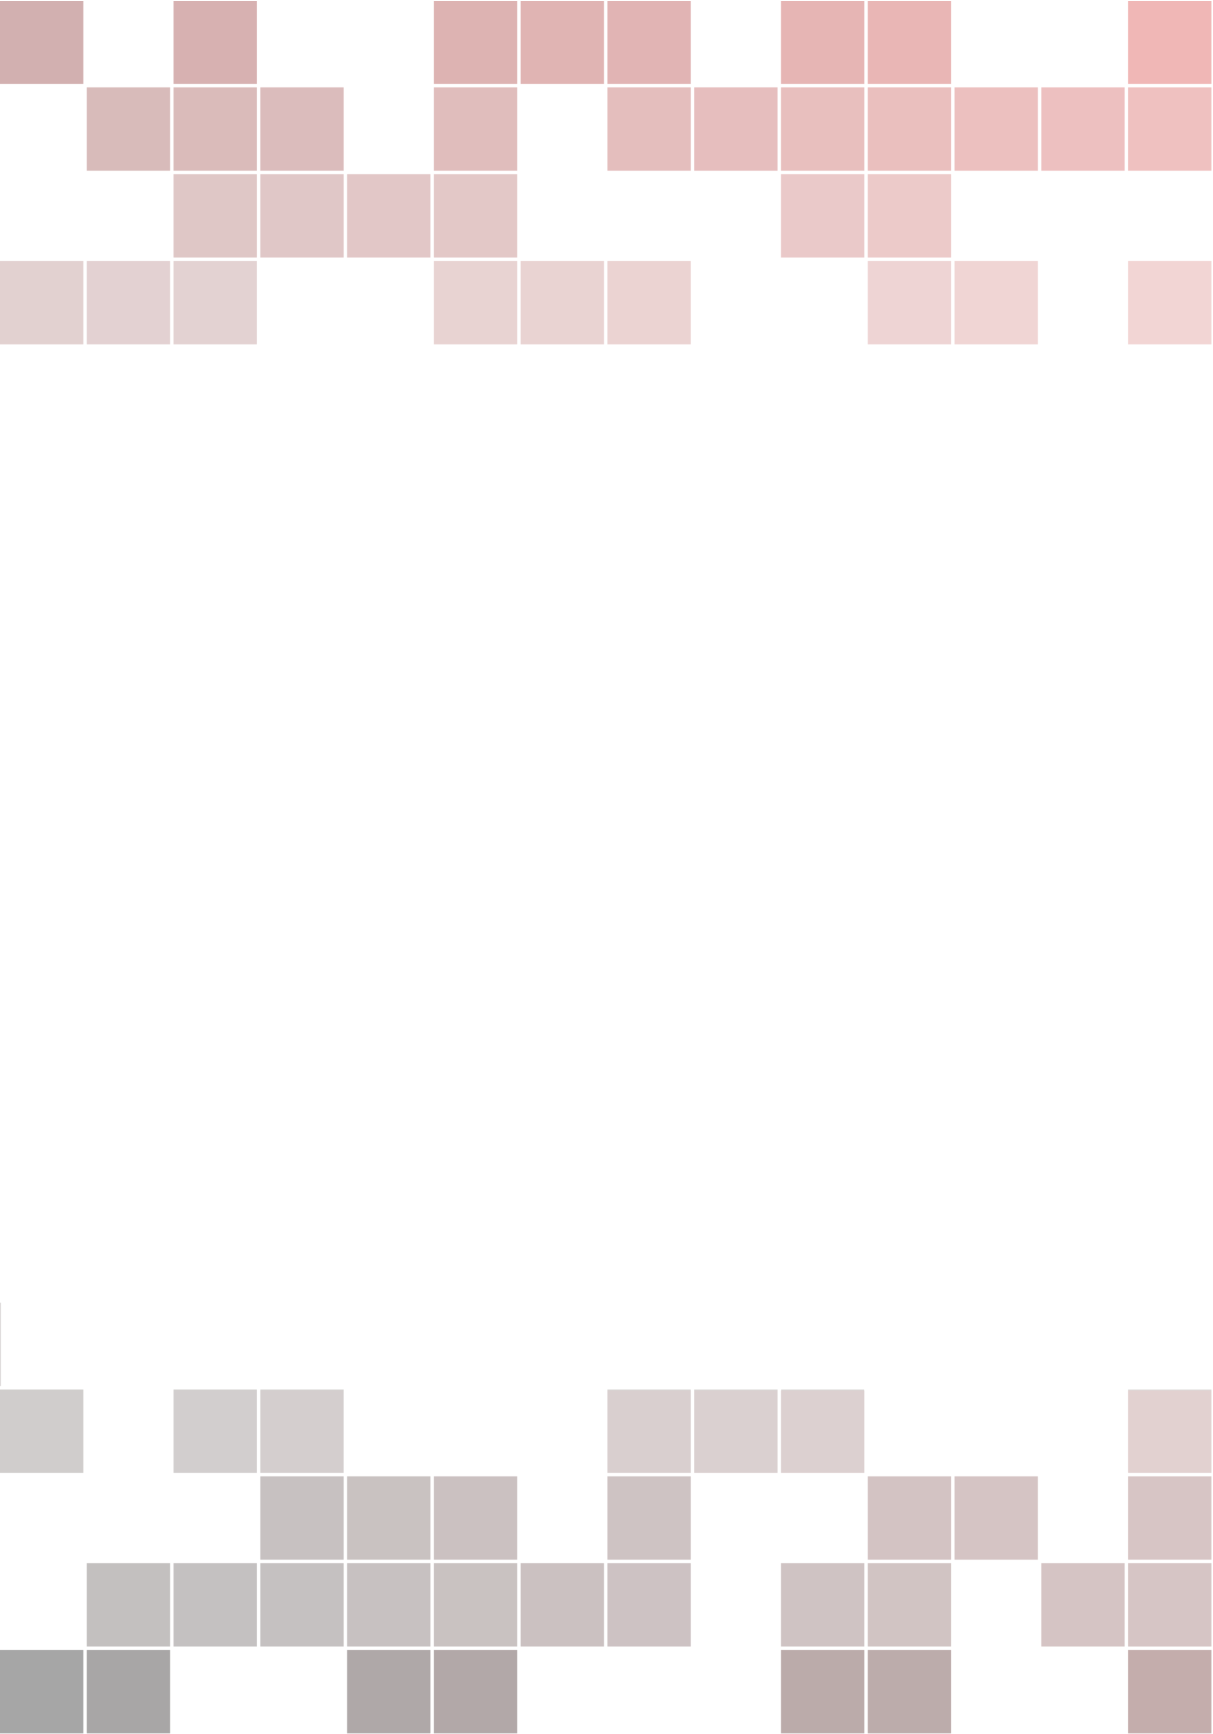
\includegraphics[width=\paperwidth]{background.pdf}} % Code to output the background image, which should be the same dimensions as the paper to fill the page entirely; leave empty for no background image
	{ % Title(s) and author(s)
		\centering\sffamily % Font styling
		{\LARGE \href{https://www.uj.ac.za/}{University of Johannesburg}\par} % Subtitle
		\vspace{16pt}
		{\large Masters Dissertation\par} % Subtitle
		\vspace{16pt} % Vertical whitespace
		{\Huge\bfseries A NEAT Inspired GEP Algorithm\par} % Book title
		\vspace{16pt} % Vertical whitespace
		% {\huge\bfseries Louis John Hassett\par} % Author name

		\begin{minipage}[t]{0.4\textwidth}
		\begin{flushleft} \large
		\emph{Author:}\\
		\href{http://www.johnsmith.com}{Louis John Hassett} % Author name - remove the \href bracket to remove the link
		\end{flushleft}
		\end{minipage}
		\begin{minipage}[t]{0.4\textwidth}
		\begin{flushright} \large
		\emph{Supervisor:} \\
		\href{http://www.jamessmith.com}{Prof. Duncan A. Coulter} \\ % Supervisor name - remove the \href bracket to remove the link  
		\emph{Co-supervisor:} \\
		\href{http://www.jamessmith.com}{Daniel Ogwok}
		\end{flushright}
		\end{minipage}\\[1cm]

		\large \textit{A dissertation submitted in fulfillment of the requirements\\ for the degree of Master in Computer Science}\\[0.3cm] % University requirement text
		\textit{in the}\\[0.4cm]
		\href{https://adam.uj.ac.za/academy/}{Faculty of Science\\Academy of Computer Science and Software Engineering}\\ % Research group name and department name
	}


%----------------------------------------------------------------------------------------
%	COPYRIGHT PAGE
%----------------------------------------------------------------------------------------

\thispagestyle{empty} % Suppress headers and footers on this page

\noindent\enquote{\itshape It is not the strongest of the species that survives, nor the most intelligent that survives. It is the one that is most adaptable to change. In the struggle for survival, the fittest win out at the expense of their rivals because they succeed in adapting themselves best to their environment.}\bigbreak

\hfill Charles Darwin


~\vfill % Push the text down to the bottom of the page

\noindent \textbf{Acknowledgements} \\
<TODO> - Add acknowledgements here


%----------------------------------------------------------------------------------------
%	TABLE OF CONTENTS
%----------------------------------------------------------------------------------------

\pagestyle{empty} % Disable headers and footers for the following pages

\tableofcontents % Output the table of contents

\listoffigures % Output the list of figures, comment or remove this command if not required

\listoftables % Output the list of tables, comment or remove this command if not required

\pagestyle{fancy} % Enable default headers and footers again

\cleardoublepage % Start the following content on a new page

%----------------------------------------------------------------------------------------
%	SECTIONING EXAMPLES CHAPTER
%----------------------------------------------------------------------------------------
%------------------------------------------------
\chapterimage{}
\chapterspaceabove{6.75cm} 
\chapterspacebelow{7.25cm}
\chapter{Introduction}\index{chapter:introduction}
\section{Background}
The theory of evolution by natural selection, first introduced by Charles Darwin, has profoundly influenced our understanding of the life and adaption in the natural world. Darwin's insight that species evolved over generations through the survival and reproduction of individuals with advantageous traits has not only shaped the biological sciences, but has also inspired computational models that emulate these adaptive processes (\cite{basicsOfEvolutionaryComputing}). Over millions of years, evolution has given rise to complex biological systems, among which the human brain stands as one of the most intricate. Composed of billions of neurons, the brain processes information through electrochemical signaling across complex interconnected networks, enabling perception, reasoning, and decision-making (\cite{engelbrecht2007computational}). These biological mechanisms have served as a blueprint for the development of artificial intelligent systems, particular in the field of evolutionary computation and neural networks.

\parbreak

\noindent In computer science, evolutionary algorithms simulate the process of natural selection to solve complex optimisation problems. These algorithms operate on populations of candidate solutions, applying genetic operators such as mutation, crossover, and selection to iteratively improve the problem's solution. In conjunction to the expanding field of evolutionary computing, artificial neural networks (ANNs) which are inspired by the structure and function of biological neurons have become foundational in machine learning. These networks consist of interconnected nodes that process information in layers, enabling machines to learn from data and perform tasks such as classification, prediction, and control (\cite{russell2016artificial}). The intersection of evolutionary algorithms and neural networks has given rise to the field of neuroevolution, which seeks to evolve both the structure and parameters of neural networks using evolutionary principles.

\parbreak

\noindent Among the many algorithms developed within the field of evolutionary computing and neuroevolution, Gene Expression Programming (GEP) and the NeuroEvolution of Augmenting Topologies (NEAT) stand out due to their unique and complementary approaches to evolving computational structures. Gene Expression Programming (GEP) is an evolutionary algorithm that evolves computer programs or symbolic expressions. It represents solutions as linear chromosomes, which are then expressed as expression trees through an effective genotype-to-phenotype mapping scheme. This approach allows the evolution of tree-like structures in a more robust and flexible manner than traditional genetic programming techniques (\cite{ferreira2006gene}). NEAT, in contrast, focuses on evolving the topology and weights of neural networks. It introduces several key innovations, including historical markings (innovation numbers) to track structural changes, speciation to preserve diversity within the population, and incremental growth of network complexity to efficiently explore the search space. These features enable NEAT to evolve increasingly sophisticated neural architectures over time (\cite{stanley2002evolving}).

\parbreak

\noindent This dissertation introduces a novel hybrid algorithm, GEP-NEAT, which seeks to combine the structural expressiveness of GEP with the adaptive topology evolution of NEAT. The motivation for developing GEP-NEAT arises from specific limitations observed in both NEAT and GEP-based neural network approaches. While NEAT has demonstrated success in evolving neural network topologies, it suffers from computational inefficiencies, particularly due to the overhead introduced by topological sorting during network evaluation which becomes increasingly problematic as networks grow in complexity. On the other hand, GEP-NN, an approach that applies GEP to evolve neural networks, offers promising alternative by representing neural structures as expression trees, but it remains relatively underexplored in the literature and lacks the methodological maturity and empirical validation seen in other neuroevolutionary techniques. GEP-NEAT is proposed a response to these challenges, aiming to combine the structural flexibility of GEP with the evolutionary dynamics of NEAT. At the heart of GEP-NEAT is a new representation scheme in which innovation numbers are encoded as sub-tree configurations. This approach allows for a more expressive and hierarchical encoding of neural structures, facilitating the reuse of functional subcomponents and promoting the emergence of modular architectures. By integrating GEP's symbolic representation with NEAT's evolutionary dynamics, GEP-NEAT aims to provide a more powerful and flexible tool for evolving neural networks.

\section{Structure}
This dissertation begins with this introductory chapter, which outlines the research motivation, and key research questions. It also highlights the academic contributions of the work, including publications that have emerged from the research process. Following the introduction, a dedicated chapter is presented on the research methodology, which adopts a design science approach. This chapter details the methodological framework used to guide the development, implementation, and evaluation of the proposed algorithm.

\parbreak

\noindent The core of the dissertation presents a comprehensive literature review, divided into three chapters. The first of these explores the foundations of evolutionary computing, providing context for the broader field in which the work is situated. The focuses on neuroevolution, examining how evolutionary algorithms have been applied to the development of neural networks. The third chapter delves into gene expression programming, detailing its mechanisms, advantages, and relevance to the proposed approach.

\parbreak

\noindent After establishing the theoretical foundation, the dissertation introduces the GEP-NEAT algorithm in detail. This chapter covers the theoretical underpinnings of the algorithm, its practical implementation, and the experimental setup used to evaluate its performance. The results of these experiments are then presented and analysed, with a focus on assessing the algorithm's effectiveness, efficiency, and potential advantages over existing methods. The final chapter concludes the dissertation by summarising the key findings, discussing their implications, and outlining directions for future research.

\section{Research Questions}
The development of algorithms that evolve neural network architectures remains a dynamic and evolving area of research. While various approaches have been proposed to automate the design of neural networks through evolutionary computation, several open questions persist regarding the efficiency, expressiveness, and adaptability of these methods. This dissertation is driven by a set of research questions that aim to explore and address specific limitations in existing neuroevolutionary techniques, particularly GEP and NEAT.

\parbreak

\noindent The first research question investigates the structural limitations of current gene expression programming when applied to neural networks. Traditional neural networks typically include architectural features such as bias nodes and non-linear activation functions, which are essential for enhancing representational capacity. However, many implementations of gene expression programming for neural networks do not incorporate these features. This leads to the first question:

\begin{researchquestion}{1}
    \textit{How can gene expression programming be extended to evolve neural networks that closely resemble traditional architectures, including the incorporation of bias nodes and activation functions?}
\end{researchquestion}

\parbreak

\noindent The second question addresses a known computational bottleneck in topology-based neuroevolutionary algorithms. Specifically, algorithms that evolve network structures often rely on topological sorting to ensure valid signal flow during evaluation. While effective, this process can become increasingly inefficient as networks grow in size and complexity. This raises the question:

\begin{researchquestion}{2}
    \textit{Can the computational inefficiencies associated with topological sorting in neural network evaluation be mitigated through alternative representations or evaluation strategies?}
\end{researchquestion}

\parbreak

\noindent A third area of inquiry concerns the role of innovation numbers in NEAT. Traditionally, innovation numbers are used to track structural changes and align genomes during crossover, however, this usage is largely historical and does not contribute directly to the functional behavior of the algorithm. This lead to the question:

\begin{researchquestion}{3}
    \textit{Is it possible to redefine innovation numbers in NEAT to represent meaningful and reusable structural components?}
\end{researchquestion}

\parbreak

\noindent Building on this idea, the fourth question explores the practical implications of such a redefinition. If innovation numbers can be used to encode modular structures, it is important to understand how this can be leverages to improve algorithmic performance. Thus, the next question is:

\begin{researchquestion}{4}
    \textit{Provided that innovation numbers are redefined as reusable structural components, how can this representation be exploited to improve the performance, modularity, or evolutionary dynamics of the algorithm?}
\end{researchquestion}

\parbreak

\noindent The fifth question considers the broader hypothesis that combining distinct evolutionary strategies may lead to improved outcomes. Specifically, it examines whether integrating symbolic expression-based representations (GEP) with topological representations (NEAT) can result in a more effecting approach to evolving neural networks. This gives rise to the question:

\begin{researchquestion}{5}
    \textit{Does the integration of symbolic-based representations (GEP) with topology-evolving strategies (NEAT) result in improved performance, scalability, or expressiveness compared to using either approach in isolation?}
\end{researchquestion}

\parbreak

\noindent Finally, the sixth question addresses a practical limitation in many symbolic neuroevolutionary systems, that is, the difficulty of evolving neural networks with multiple outputs. Many real-world tasks require networks to produce more than one output simultaneously, yet existing representations often struggle to accommodate this. This leads to the final question:

\begin{researchquestion}{6}
    \textit{How can expression trees be adapted to support the evolution of neural networks with multiple outputs, and what are the implications for multi-output learning tasks?}
\end{researchquestion}

\parbreak

\noindent Together, these research questions form the foundation of this dissertation. They aim to explore the theoretical and practical challenges of evolving neural networks using symbolic and structural representations, and to investigate whether new approaches can overcome the limitations in existing methods.

\section{Publications Resulting from this Work}\index{sec:publication\_from\_resulting\_work}
A peer-reviewed conference paper derived from this research was published in the proceedings of the \textbf{8th International Conference on Information Science and Systems (ICISS 2025)}. As an established forum in its eight iteration, ICISS maintains rigorous academic standards through its double-blind peer review process, where both author and reviewer identities are concealed to remove bias and ensure impartial evaluation based solely on scholarly merit. The conference brings together leading researchers across ten interdisciplinary tracks spanning artificial intelligence, data science, and information systems.

\parbreak

\noindent The accepted paper, which contributes to the Machine Learning and Artificial Intelligence track, presents the algorithm GEP-NEAT with its innovation number novelty, showcasing the ability to solve the XOR and Cart Pole problem effectively. ICISS 2025 facilitated valuable scholarly exchange through keynote presentations by field leaders, technical workshops, and interdisciplinary discussion bridging academic and real-world application. The conference proceedings are to be published into \textbf{Communications in Computer and Information Sicence (Electronic ISSN: 1865-0937 \& Print ISSN: 1865-0929)} as a proceedings book volume and indexed by EI Compendex, Scopus, INSPEC, SCImago and other databases.
%------------------------------------------------

%------------------------------------------------
\chapterimage{}
\chapterspaceabove{6.75cm}
\chapterspacebelow{7.25cm} 
\chapter{Research Methodology}\index{chapter:research\_methodology}
This chapter outlines the methodological framework used to guide the development, implementation, and evaluation of the GEP-NEAT algorithm, a novel hybrid approach that combines Gene Expression Programming (GEP) and NeuroEvolution of Augmenting Topologies (NEAT). To ensure methodological relevance, the research is structured around the Design Science research (DSR) paradigm, which supports the iterative development of innovative artifacts to be used in real-world application. This is complemented by Experimental Design, which provided a structured approach in testing and validating the generated artifact, and Quantitative Analysis which offers objective metrics for performance evaluation. This chapter is organized in three sections. The first presents the design science methodology and application. The second discusses the role of experimental design in structuring the evaluation process. The third outlines quantitative methods that can be used to assess the hybrid algorithm's performance.

\section{Design Science Research}
Design Science Research (DSR) is a research paradigm centered on the creation of innovative artifacts that contribute meaningfully to the existing body of scientific knowledge within a specific domain. According to \cite{hevner2004design}, DSR integrates the principles of relevance, rigor, and iterative design to produce solutions that are both practically useful and theoretically grounded. This methodology is particularly well-suited to algorithmic research, where the objective is to construct novel solutions and evaluate their effectiveness through cycles of design, implementation, and refinement. In the context of this research, the artifact developed is the GEP-NEAT hybrid algorithm, which aims to address the specific limitations in existing neuroevolutionary approaches by combining the strengths of GEP and NEAT. \bigskip

\noindent The use of design science as the chosen research methodology can be examined as 6 process elements as follows with reference to Figure \ref{fig:dsr}:

\begin{enumerate}
    \item \textbf{Problem identification and motivation} - The first stage's aim is to formulate the research problem and justify the necessity of a solution. Importantly, this can be broken down into smaller problems in order for the solution to better capture the problem's complexity. Providing the problem and motivation to the reader accomplishes two things, that is, the solution to the problem is motivated to be pursued and secondly, the reader has a much better understanding of what the intention behind the conducted design, development of the prototype and its respective results are.
    \item \textbf{Objectives of a solution} - The second stage of this methodology is to create a set of objectives based on the problem definition defined above. These objectives can be either, quantitative, qualitative, or both. Quantitative objectives deal with measurable outcomes that can be expressed numerically whereas qualitative objectives are difficult to quantify and focus on the quality or nature of the solution.
    \item \textbf{Design and development} - This stage deals with the creation of an artifactual solution along with detailing the artifact's functionality and architecture which will be used to create the actual artifact.
    \item \textbf{Demonstration} - This stage aims to show the efficacy of the artifact to solve the problem at hand by means of ideologies such as simulation, case studies or experimentation.
    \item \textbf{Evaluation} - This stage's aim is to measure essentially how well the created artifact supports a solution to the problem which involves the comparison of tried and tested real world results to that of the artifacts. As mentioned in the objective phase, a quantitative and qualitative approach can be taken; the quantitative comparison being based on quantifiable metrics, such as convergence speed, solution quality, etc., and the qualitative comparison being based on solution innovations, adaptability, ease of use, etc.
    \item \textbf{Communication} - The final stage is to effectively communicate the following:
    \begin{itemize}
        \item \textit{Problem and it's importance}: This will essentially be the problem statement detailed along with its justification.
        \item \textit{Artifact}: An overview of the artifact.
        \item \textit{Artifact's utility and novelty}: A background and technical literature that make up the artifact will be provided to the reader.
        \item \textit{Rigor of its design}: The way in which the newly formed algorithm/design will be detailed to the reader with explicit explanation in the intricate design choices with mentions to previous results of algorithms the prototype is based on.
        \item \textit{Effectiveness}: An analysis will be done on the constructed artifact with comparison to other existing designs using quantitative and qualitative metrics in order to showcase its use and efficacy to the research field at large.
    \end{itemize}
\end{enumerate}

\begin{figure}[H] % Use [H] to suppress floating and place the figure/table exactly where it is specified in the text
	\centering % Horizontally center the figure on the page
	\includesvg[width=\textwidth]{Figures/Chapter_Research_Methodology/rm_dsr.svg} % Include the figure image
	\caption{Design Science Research Process Diagram (adapted from \cite{hevner2004design})}
	\label{fig:dsr} % Unique label used for referencing the figure in-text
\end{figure}

\section{Olivier's Insight}
While Design Science Research (DSR) provides a high-level framework for the creation and evaluation of innovative artifact, it lacks a fixed set of operational steps or tools. To address this, \cite{olivier2009information}, have proposed complementary activities that can be integrated into the DSR process to support knowledge construction, problem exploration, and artifact validation. Each activity contributes to a different phase of the research process, from identifying the problem space to validating the proposed solution. \bigskip

\subsection{Literature Review}
\noindent The research process begins with a comprehensive review of existing literature, which serves as the foundation for identifying gaps in current knowledge and framing the research problem. In line with Olivier's view, the literature view is not a one-time task, but an ongoing process of gathering, filtering, and synthesizing information. It enables the researcher to build a solid theoretical foundation, avoid redundant approaches, and identify opportunities for innovation. \bigskip

\noindent The literature review focuses on three core areas, that is, evolutionary computation, neuroevolution, and gene expression programming. By critically analysing existing work in these domains, the review highlights the limitations of current approaches and motivates the development of a hybrid solution. In selecting sources, priority is given to peer-reviewed journal articles, followed by conference proceedings, textbook, and reputable online resources. While blogs and traditional \textit{'google'} searches are generally treated with caution and used only as a means to support academic findings. \bigskip

\noindent The literature review also serves several strategic purposes, that is, it helps to define the scope of the research problem, identify methodological approaches, avoid unproductive directions, and uncover new lines of inquiry. In the context of DSR, it provides the initial input for the design cycle by informing the development of the conceptual model and guiding the evaluation criteria for the artifact designed.

\subsection{Conceptual Modeling}
Once the research problem is clearly defined, the next step is to develop a conceptual model that captures the essential components of the proposed solution. In this context, a model serves as a structured representation of the system or process under investigation. It helps to clarify boundaries of the solution space, and provide a blueprint for implementation. \bigskip

\noindent \cite{olivier2009information}, emphasises that models can take various forms depending on the research context. They may be descriptive, metaphorical, or formal, and can be developed using principles, scientific notation, or visual languages. This research employs Unified Modeling Language (UML) diagrams to achieve this as it provides a standardised and widely accepted visual language for representing architecture and behavior (\cite{koc2021uml}). The diagrams used include:
\begin{itemize}
    \item \textbf{Class and component diagrams}: These diagrams represent the structural composition of the algorithm.
    \item \textbf{Activity diagrams}: These diagrams illustrate the flow of control and decision-making processes.
    \item \textbf{Sequence diagrams}: These diagrams show interactions between components during execution.
\end{itemize}

\noindent UML diagrams are chosen for their clarity and ability to convey complex system interactions in a digestible format, ensuring that the model is comprehensible to both technical and academic audiences. In line with \cite{olivier2009information} perspective, models in computer research can be developed through various means, including formal specification, metaphorical representation, or practical design. In this research, the model is primarily constructed through design, using system architecture and algorithmic logic to represent the proposed solution. Where appropriate, descriptive metaphors are used to explain abstract concepts, and formal notation is employed to define algorithmic behavior.

\subsection{Prototype Development}
With the conceptual model in place, the next step is to construct a working prototype that embodies the proposed solution. In DSR, the prototype serves as a tangible instantiation of the model and provides a means of validating the design through various test and benchmarking mechanisms. As noted by \cite{olivier2009information}, a prototype is not merely a demonstration tool but a vehicle for inquiry. This allows the researcher to explore the behavior of the system, identify limitation, and refine the design based on feedback. \bigskip

\noindent Prototypes are also recognized as essential tools for reducing uncertainty and improving design outcomes. \cite{camburn2017design}, highlight that prototyping enables real-time feedback, supports iterative development, and facilitates the early identification of design flaws. This allows researchers to test algorithmic behavior under realistic conditions and to make data-driven decisions about further development. Other research indicates that prototypes provide proof by construction, offering concrete evidence that a theoretical model can be realized in practice. They simply serve as a foundation for further experimentation and analysis, particularly in exploratory research where the goal is to uncover new insights or validate emerging paradigms (\cite{nunamaker1990systems}).

\subsection{Experimental Evaluation}
The final activity in the research process is the empirical evaluation of the prototype. \cite{olivier2009information}, emphasises that experiments in computing research can serve multiple purposes, that is, they can be used to test hypotheses, explore parameter spaces, or validate theoretical models. \bigskip

\noindent The evaluation of the prototype is approached through both quantitative and qualitative methods, inline with DSR principles of the artifact being rigorously tested to validate the effectiveness in solving the identified problem. Quantitative evaluation in this research involves measuring the algorithm's performance using standard metrics such as accuracy, precision, convergence speed, and computational efficiency (\cite{gregar2023research}).  Complementing this, qualitative evaluation focuses on the artifacts structural and functional qualities such as modularity, innovation, and scalability. \cite{olivier2009information} notes that qualitative insights are crucial for understanding how well a prototype aligns with its conceptual model and whether it contributes meaningfully to the body of knowledge.

\section{Conclusion}
By integrating literature review, conceptual modeling, prototype development, and experimental into the DSR framework along with Olivier's insight, this research adopts a comprehensive and methodological rigor approach to artifact construction. Each activity contributes to a different phase of the design cycle and supports overarching goal of developing a novel, effective, and theoretically grounded solution to the problem of evolving neural network architectures. The result is a research process that is capable of producing meaningful contributions to both theory and practice.
%------------------------------------------------

%------------------------------------------------
\chapterimage{}
\chapterspaceabove{6.75cm}
\chapterspacebelow{7.25cm} 
\chapter{Evolutionary Algorithms}\label{chapter_ea}\index{Evolutionary Algorithms}

\noindent This chapter provides the reader with a comprehensive overview of what evolutionary algorithms entail along with a representative selection of existing work. An introduction to evolutionary algorithms is first given in Section \ref{ea_introduction}. Section \ref{historical_background} paints a picture of the historical background of evolutionary algorithms. The reader is then provided with fundamentals behind evolutionary algorithms in Section \ref{sec:ea_core_concepts}. Section \ref{sec:ea_types_of_ea} reviews the different evolutionary algorithms that exist and their differences, and finally Section \ref{sec:ea_current_research} provides an overview of current advancements in the field of evolutionary computation.

\section{Introduction}\label{ea_introduction}
Evolutionary Algorithms (EAs) belong to a large group of optimisation methods that take inspiration from Darwinian biological evolution (\cite{book_introduction_to_evolutionary_computing}). These methods replicate processes like natural selection, mutation, and reproduction. They simulate the adaptive and competitive dynamics observed in nature, where a set of candidate solutions, called the population, is iteratively refined over multiple generations (\cite{basicsOfEvolutionaryComputing}). 

\parbreak

\noindent In order to mimic the lifecycle of organisms, selecting a representation of a candidate solution that is amenable to algorithmic manipulation is a prerequisite. With the proper representation of a candidate solution in place, EAs follow the general framework of mimicking the lifecycle of organisms. To explain simply, this framework works firstly by generating an arbitrary number of handful candidate solutions that make up the initial population. Each candidate solution will have an attempt at solving the problem at hand after which this attempt will be scored and recorded relative to a particular fitness. This scoring scheme is achieved by a \textit{fitness function} and generally has the primary role of determining how strong an individual is at solving the problem at hand. Each candidate solution will then go through a selection process whereby the best solution will be chosen, and the others disregarded, ensuring that only the best-performing candidates pass their desirable traits onto offspring and consequently forthcoming generations. Additionally, a mechanism is established to combine candidate solutions, facilitating the exchange of traits to enhance the diversity and quality of the population over successive iterations. Surviving candidates will produce offspring by applying genetic operators such as mutation (which introduces variability by altering the gene of offspring) and crossover (which combines the traits from two or more parents). After population initialization, this repetitive process of selection, mutation, and reproduction enhances the likelihood that the successive generations migrate towards a global optima while mitigating the chances of falling into a local optima (\cite{evolutionaryComputingAndNeuralNetworks}). 

\parbreak

\noindent EAs have been applied to a wide range of different fields ranging from engineering, to artificial intelligence. EAs are typically used in optimisation problems where there is a single or multiple objectives due to their ability to explore the solution space in a flexible manner. EAs have application in a vast number of fields where for example EA algorithms were used to optimise solar panel layouts in real-time by aircrafts in the engineering realm. Another example was EAs involvement to predict flood routing in natural channels using gene expression programming (GEP) in the environmental field (\cite{slowik2020evolutionary}).

\section{Historical Background}\label{historical_background}
EAs go back to the early computational era of the 1950s and 60s where researchers began to draw inspiration from Darwinian principles of natural selection (\cite{alainsanaEvolutionaryAlgorithms}). These researchers managed to mathematically model the competitive and adaptive processes found in nature in order to solve and optimise complex and multi-dimensional problems. The idea was simple - just as organisms in nature evolve to adapt according their environment, organisms in the mathematical realm (candidate solutions) can \textit{"evolve"} by competing and improving over time, akin to  natural generations. This approach in solving optimisation problems became compelling to be used in problems that were ill-defined or had far too many variables that lead to exhaustive searching and suboptimal solutions. 

\parbreak

\noindent EAs began with contributions from many important people. British mathematical and geneticist Alex Fraser took early steps to model genetic ideas using computers in the 1950s (\cite{links2002alex}). Hans-Paul Schwefel and Ingo Rechcenberg were inspired by his work and soon developed evolution strategies in Germany during the 1960s primarily for application in engineering (\cite{alainsanaEvolutionaryAlgorithms}). Around that time, an American Scientist, John Holland, formulated the concept of genetic algorithms (GAs) which established a formal framework to simulate biological evolution in a mathematical sense. Holland's work in the 1970s revolutionized EAs extending their application in many areas (\cite{alainsanaEvolutionaryAlgorithms}). After the publication of the book, \textit{Genetic Algorithms in Search, Optimisation and Machine Learning} by E. Goldberg in 1989, interest in the field became much more widespread (\cite{alainsanaEvolutionaryAlgorithms}).

\parbreak

\noindent As the field of computers evolved in terms of technological sophistication and breadth of application, so did the capabilities and appeal of evolutionary algorithms. Due to advancements in computer science in the late 20th century, researchers began to explore more complex and sophisticated EA models. Also PhD student of John Holland, John Koza, a computer science researcher, formulated genetic programming which opened new avenues for using evolution to optimise non\-linear structures such as symbolic regression functions and tree\-like structures (\cite{koza1994genetic}). Differential Evolution (DE) was introduced in the 1990s which provided a mechanism in solving problems suited for continuous parameter optimisation (\cite{das2010differential}).

\section{Core Concepts in Evolutionary Algorithms}\label{sec:ea_core_concepts}
EAs are built from several core concepts that mimic Darwinian principles, that is, the process of selection, variation, and inheritance. These core elements form the backbone of the way in which EAs operate, creating a system whereby candidate solutions are evolved over iterative generations to meet or exceed a given objective. Understanding these core concepts are crucial in understanding the mechanics and flexibility of EAs, as each component dictates how the algorithm explores and optimises the search space.

\begin{figure}[H] % Use [H] to suppress floating and place the figure/table exactly where it is specified in the text
	\centering % Horizontally center the figure on the page
	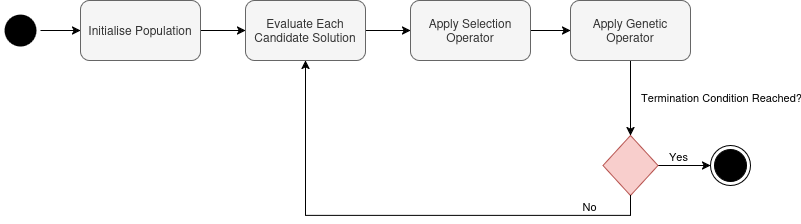
\includegraphics[width=\textwidth]{Figures/chapter_ea/chapter_ea_ea_framework.png} % Include the figure image
	\caption{Evolutionary Algorithm Framework (adapted from \cite{handsOnGeneticAlgorithms})}
	\label{fig:ea_framework} % Unique label used for referencing the figure in-text
\end{figure}

\subsection{Representation}
The term chromosome is often used to refer to representations of candidate solutions within the population which are a critical aspect of the evolutionary algorithms, an attempt to model genes and chromosomes seen in nature. The representation dictates how individuals are encoded, manipulated, and evaluated within the evolutionary process. A representation that is well-defined within the context of the optimisation problem enhances the algorithm's ability to explore the search space efficiently while maintaining diversity and feasibility among solutions.

\parbreak

\noindent The genotype-phenotype mapping translates encoded information into a meaningful solution. There are two forms in an evolutionary algorithm, namely, the \textbf{genotype} which is the encoded representation of a solution and is typically manipulated directly by genetic operators such as crossover and mutation, and the \textbf{phenotype} which is the decoded, functional representation of the solution which is what gets evaluated against the fitness function or objective (\cite{okramergeneticalgorithms}). For example, consider an optimisation problem where a 4-bit binary number that decodes the highest integer value needs to be found. The genotype would be a chromosome representing a 4-bit string (e.g., $1010$). The phenotype would be the decoded integer value (e.g., $1010 \rightarrow 10$ in decimal). It is not necessarily for every optimisation problem to have an explicit genotype-phenotype mapping, in particular, when the genotype is the solution itself (\cite{okramergeneticalgorithms}).

\parbreak

\noindent There are many ways in which chromosomes can be represented as solutions to the problem at hand. Representations are divided into two categories, namely, direct representations and indirect representations. Direct representations are those in which the genotype-phenotype mapping is one-to-one, allowing genetic operators to be applied directly without transformation. In contrast, indirect representations require an additional decoding step to map genotypes to phenotypes before genetic operators can be applied (\cite{rothlauf2009representations}). Genetic algorithms have originally been proposed to be binary coded to mimic the genetic material of natural organisms, however, different representations are used based contextually on the optimisation problem at hand (\cite{yu2010introduction}). Common representations include those seen in Figure \ref{fig:ea_representations}. Binary representations are commonly used for problems with discrete or combinatorial solutions, such as feature selection or Boolean optimisation, where each bit can encode the presence/absence of a feature or a binary decision. Integer or real-valued representations are suited for numerical optimisation tasks, such as parameter tuning in machine learning or engineering design, where variables require fine-grained precision. Tree-based representations model hierarchical structures, making them ideal for symbolic regression, program synthesis, or parsing tasks, where solutions naturally map to decision trees or recursive expressions.

\begin{figure}[h!] % Use [H] to suppress floating and place the figure/table exactly where it is specified in the text
	\centering % Horizontally center the figure on the page
	\includesvg[width=\textwidth]{Figures/chapter_ea/chapter_ea_representation.svg} % Include the figure image
	\caption{Common Gene Representation (adapted from \cite{intelligentOptimization})}
	\label{fig:ea_representations} % Unique label used for referencing the figure in-text
\end{figure}

\subsection{Population and Fitness}
The starting point in any evolutionary algorithm is the initialization of a population as shown in Figure \ref{fig:ea_framework} which represents a group of candidate solutions that could potentially solve the problem at hand. Unlike traditional optimisation techniques which mainly focus on a single-solution pathway, EAs work within the entire solution space by means of parallelism (\cite{okramergeneticalgorithms}). To put it simply, each generation evaluates candidate solutions as potential answers, with the algorithm progressively identifying better ones through selection and variation. This parallel search ensures that local optima are avoided, an issue which high-dimensional optimisation typically face. By ensuring that the initial population generated is diversified, there is an increased chance of finding a global or near global optimal solution. There are many methods for initializing a population, with randomized approaches being the most common, specifically those drawn from a uniform probability distribution, to ensure a broad coverage of the search space (\cite{initialPopulation}). Other mechanisms for initializing the population include heuristic and intelligent based approaches when existing solutions are known which could potentially ensure a better coverage spread of the search space (\cite{initialPopulation}). When taking advantage of using existing solutions to explore the search space, repetitive computations are mitigated yielding in an increased efficiency. Likewise, non-random initial populations can directly gear the algorithm to search a particular region of the solution space from the beginning which again, with the aid of known solutions, can allow the algorithm to converge quicker towards an optimal solution. Other mechanisms include deterministic based approaches in which candidate solutions are generated in a more controlled and evenly distributed manner leading to a better coverage of the solution space (\cite{THARWAT2021100952}).

\parbreak

\noindent In genetic algorithms, diversity refers to the variety of genetic material (e.g., different solution features or values) within a population. The population's diversity closely relates to how well the candidate solutions explore the search space. If individuals are too similar, they lack diversity leading to premature convergence causing stagnation around a suboptimal solution. Conversely, if the individuals are too diverse from one another, convergence can be delayed meaning that more generations are needed in order to hone in on an optimal solution (\cite{okramergeneticalgorithms}). A fine balance is therefore needed between exploration and exploitation. A highly diverse initial population is crucial to ensure thorough exploration of the search space early in the optimisation process. As generations progress, the algorithm selectively converges toward higher-quality solutions, naturally reducing diversity while refining the best candidates. There are well studied mechanisms which can control this balance such as mutation rate adjustment, niche-reserving mechanisms, or even hybrid approaches. Using these mechanisms ensures that both diversity and convergence can be capitalized.

\parbreak

\noindent With reference to Figure \ref{fig:ea_framework}, after the population is initialized, each candidate solution will be vetted by means of a fitness function which is a mathematical measure that scores how well the candidate solution meets the objective (\cite{okramergeneticalgorithms}). \todo[color=yellow]{"The fitness function needs to be discussed much earlier than this" $\rightarrow$ I am trying to follow the thought process of Figure \ref{fig:ea_framework} by following the flow diagram. I thought this may be easier to introduce for the reader.} This score reflects the quality of the candidate solution in regard to the optimisation goal and is used to guide the selection process in subsequent generations. For example, given an optimisation problem such that $x$ is an integer to maximize the parabolic equation $f(x) = -x^2 + 25$, the fitness function would be taking a candidate solution, and feeding it as input into this equation. Evidently, the maximum fitness to this function would be $5$. Fitness functions are defined in different ways depending on the application at hand, for example, in engineering design problems, fitness may represent efficiency, structural stability, or cost-effectiveness, whereas in artificial intelligence, fitness could measure a predictive accuracy. The way in which a fitness function is defined shapes how effectively the EA converges towards an optimal solution, especially in multi-objective problems (MOPs) where the fitness needs to account for multiple goals (\cite{book_introduction_to_evolutionary_computing}).

\parbreak

\noindent MOPs are mathematical problems that involve optimizing multiple conflicting objectives at the same time. The fitness function in this regard is defined by the algorithm's performance in relation to these conflicting objectives as opposed to one (\cite{okramergeneticalgorithms}). A common approach in formulating the fitness function is by aggregating all the objectives in a singular fashion by means of a weighted sum (\cite{okramergeneticalgorithms}). Another approach in defining the fitness function appropriately is by changing the structure of algorithm by means of co-evolution - instead of evolving a single population, the problem is broken down into smaller problems which in turn have their own population which is evolved (\cite{ZHOU201132}). In multi-objective optimisation problems which are common in economics and engineering, the fitness function may use methods like Pareto front optimisation which balances competing objectives without forcing single trade-off solutions. Pareto optimality describes a solution that cannot be improved in any objective without degrading another. In these kind of scenarios, EAs evolve a population of solutions that collectively represent a spectrum of optimal trade-offs, giving the decision-maker flexibility in choosing the most suitable solution based on contextual priorities (\cite{rachmawati2009multiobjective}). EAs are therefore robust and versatile in solving both single and multi-objective problems which can often be riddled with narrowly defined and complex optimisation challenges.

\subsection{Genetic Operators}\label{label:ea_genetic_operators}
In EAs, genetic operators - crossover and mutation - serves as crucial mechanisms by means of variation and adaption to guide the exploration of the solution space while refining existing solutions. Variation in evolution can be divided into two types based on their arity, namely, unary (mutation) and n-ary (recombination) both of which produce offspring (\cite{book_introduction_to_evolutionary_computing}). These operators mimic the evolutionary processes seen in nature among organisms, where gene recombination and mutation introduce new traits that contribute to a population's overall fitness and adaptability (\cite{handsOnGeneticAlgorithms}).

\subsubsection{Crossover}
Crossover is an evolutionary process based on sexual reproduction whereby genetic material from two parents are combined to produce offspring that inherit characteristics from both (\cite{okramergeneticalgorithms}). Crossover plays a crucial part in diversifying the algorithm's search path by combining beneficial traits and thereby ideally producing offspring with improved fitness. There are different ways in which crossover can occur which provide varying levels of control over the inheritance process. For simplicity, consider linear gene representations for the following crossover mechanisms:

\parbreak

\noindent \textbf{Single-point Crossover} selects a single point along the chromosome and exchanges genetic material on either side as shown in Figure \ref{fig:singlepoint}. This simple approach works well when minor structural adjustments results in significant improvement (\cite{intelligentOptimization}).
	
\begin{figure}[H] % Use [H] to suppress floating and place the figure/table exactly where it is specified in the text
	\centering % Horizontally center the figure on the page
	\includesvg[width=\textwidth]{Figures/chapter_ea/chapter_ea_singlepoint.svg} % Include the figure image
	\caption{Single-point crossover}
	\label{fig:singlepoint} % Unique label used for referencing the figure in-text
\end{figure}

\noindent \textbf{Multi-point crossover} introduces more than one cutoff point, allowing for more complex combinations of genetic material from each parent thereby creating a more diverse offspring as shown in Figure \ref{fig:multipoint} (\cite{crossoverMethods}). Multi-point crossover is typically used in scenarios that are non-linear. 
	
\begin{figure}[H] % Use [H] to suppress floating and place the figure/table exactly where it is specified in the text
	\centering % Horizontally center the figure on the page
	\includesvg[width=\textwidth]{Figures/chapter_ea/chapter_ea_multipoint.svg} % Include the figure image
	\caption{Multi-point crossover}
	\label{fig:multipoint} % Unique label used for referencing the figure in-text
\end{figure}

\noindent \textbf{Uniform crossover} selects each gene randomly from one of the corresponding genes of the parent as shown in Figure \ref{fig:uniform} (\cite{crossoverMethods}). This technique produces highly diversified offspring and is suitable when seeking greater diversity in the population thereby leveraging exploration.
	
\begin{figure}[th] % Use [H] to suppress floating and place the figure/table exactly where it is specified in the text
	\centering % Horizontally center the figure on the page
	\includesvg[width=\textwidth]{Figures/chapter_ea/chapter_ea_uniform.svg} % Include the figure image
	\caption{Uniform crossover}
	\label{fig:uniform} % Unique label used for referencing the figure in-text
\end{figure}

\noindent In scenarios where problem requirements are specific, crossover strategies can be tailored to meet particular constraints. For example, order crossover (OX1) is useful for optimisation problems such as the traveling salesman problem whereby maintaining certain order relationships between genes (cities) is critical (\cite{tsp}). Such customized crossover methods ensure that the offspring retain problem-specific constraints while still inheriting the most desirable traits from parent solutions. Beyond sexual recombination, horizontal gene transfer (HGT), inspired by bacterial gene exchange, can also diversify populations by transferring genetic material directly between solutions without parent-offspring relationships (\cite{hgt}).

\subsubsection{Mutation}\label{sec:ea_mutation}
Mutation in contrast to crossover introduces randomness in the algorithm by altering one or more genes in an individual's chromosome in order to create new traits and variation (\cite{evolutionaryComputingAndNeuralNetworks}). Mutation serves as the primary source of diversity within the population and important when solutions begin to become too familiar, a condition known as \textit{genetic drift} (\cite{advancesInEvolutionaryAlgorithms}). When individuals become too similar, this results in stagnation around suboptimal solutions causing convergence towards a local maxima. Mutation can occur in many ways, such as:

\parbreak

\noindent \textbf{Bit-flip mutation (aka bitwise mutation)} is applied to chromosomes represented in binary whereby each gene has a probability that its bit is inversed (changing from 0 to 1 or vica-versa) as shown in Figure \ref{fig:bitflip} (\cite{intelligentOptimization}).
	
\begin{figure}[H] % Use [H] to suppress floating and place the figure/table exactly where it is specified in the text
	\centering % Horizontally center the figure on the page
	\includesvg[width=\textwidth]{Figures/chapter_ea/chapter_ea_bitflip.svg} % Include the figure image
	\caption{Bit-flip mutation}
	\label{fig:bitflip} % Unique label used for referencing the figure in-text
\end{figure}

\noindent \textbf{Gaussian mutation} is applied to real valued chromosomes whereby a random gene is selected and a Gaussian distribution applied by means of the function below where $x_{i}^{i}$ is the offspring, $\sigma$ is a fixed parameter for all variables, $[b_{i}, a_{i}]$ represents the range of random gene, $erf^{-1}$ represents the inverse of $erf$ which is the Gauss error function, defined by $erf(y) = \frac{2}{\sqrt{\pi}}\int^{y}_{0}e^{-t^2}dt$ (\cite{bell2022applicationsgaussianmutationself}, \cite{gaussianMutation}). Gaussian mutation allows for controlled but continuous alterations.
\begin{equation}
	x_{i}^{'} = \sqrt{2} \sigma(b_{i} - a_{i}) erf^{-1}(u^{'}i)
\end{equation}

\parbreak

\noindent \textbf{Inversion mutation} selects a subset of genes and inverts the position as shown in Figure \ref{fig:inversion}. This mutation scheme is useful in combinatorial optimisation problems where the specific arrangement of elements matters such as the travelling salesman problem (\cite{intelligentOptimization}).
	
\begin{figure}[H] % Use [H] to suppress floating and place the figure/table exactly where it is specified in the text
	\centering % Horizontally center the figure on the page
	\includesvg[width=\textwidth]{Figures/chapter_ea/chapter_ea_inversion.svg} % Include the figure image
	\caption{Inversion mutation}
	\label{fig:inversion} % Unique label used for referencing the figure in-text
\end{figure}

\noindent The parameters that govern genetic operators do not have to be static. There is more complex EAs, these parameters can be adjusted dynamically as the algorithm progresses. Adaptive mutation rates for example can be useful in maintaining diversity during later stages of the search when converging towards an optima is prioritized. Likewise, crossover rates could increase when diversity is low in order to ensure that favourable genetic material continues to recombine as the algorithm refines its search (\cite{meyer2007self}). In hybrid approaches, self-adaptive genetic operators are used whereby the parameters of mutation and crossover evolve and form part of the chromosome, allowing the EA to essentially learn optimal rates over time based on the fitness at hand (\cite{meyer2007self}). 

\parbreak

\noindent Hybrid approaches in genetic operators have become popularized due to its powerful nature. For example, memetic algorithms combine the typical genetic operators described above with local search techniques which allow candidate solutions to further refine the search space by means of exploiting problem-specific knowledge or heuristics (\cite{neri2012memetic}). This combination is useful in complex landscapes where small local improvements can lead to an increased fitness score after major variations have been introduced through crossover and mutation in individuals. Hybrid genetic operators can therefore enhance the EAs ability to explore local optima thoroughly while still retaining a broad search capacity.

\parbreak

\noindent There is a fine balance between crossover and mutation in the efficacy of EAs. Mutation ensures that the EA explores new possibilities and avoids premature convergence while crossover allows the search space's best regions to be explored by recombining favourable traits of candidate solutions. These operators form a dynamic balance between exploration and exploitation, equipping EAs with the necessary flexibility to solve complex and non-linear optimisation landscapes.

\subsection{Selection Mechanisms}\label{sec:selection_mechanisms}
Selection occurs in an evolutionary process in two instances - parent selection and survivor selection. Parent selection has its primary purpose in distinguishing individuals based on their quality in order to allow better individuals to become parents of the next generation (\cite{handsOnGeneticAlgorithms}). Survivor selection, similar to parent selection, aims to distinguish individuals apart based on quality. Parent selection occurs before variation operators are applied while survivor selection occurs after offspring are produced and evaluated against the fitness function (\cite{book_introduction_to_evolutionary_computing}). This selection mechanism mimics the natural selection seen in nature where animals with desirable traits have increased likelihood of producing better offspring - akin to this, candidate solutions with better fitness scores are more likely to produce better quality offspring to solve the objective at hand. An effective selection mechanism will ensure that there is a balance between promoting high-quality solutions whilst maintaining population diversity ideally driving the EA towards a global optimum. Below are common selection mechanisms that are typically used within evolutionary algorithms:

\parbreak

\noindent \textbf{Fitness-proportionate selection} which is one of the simplest yet most renowned selection methods. In this selection approach, each candidate solution's probability of being selected is proportional to its fitness score relative to the total fitness of the population (\cite{shukla2015comparative}). Mathematically, the probability that each individual is selected is given by the formula below where $f_x$ is the fitness of individual $x$ (\cite{shukla2015comparative}).
\begin{equation}
	p_x = \frac{f_x}{\sum^{n}_{i=1}f_i}
\end{equation}
This selection mechanism is computationally efficient ($O(n)$ complexity) and ensures that fitter individuals are more likely to survive and reproduce while still giving less fit individuals the chance to contribute and preserve genetic diversity thereby preventing stagnation. The most common implementation of this approach is \textit{roulette-wheel selection}, which assigns selection probabilities analogously to slots on a roulette wheel such that higher fitness solutions occupy larger wheel segments and thus have greater likelihood of being selected. Although this process is simple, this mechanism may suffer from genetic drift if highly fit individuals dominate which results in a loss of diversity in subsequent generations. This approach raises considerations about the \textit{takeover time}, that is, the number of generations required for the best candidate solution's genes to dominate the population under selection pressure alone. Short takeover times indicate strong selection pressure that may lead to premature convergence, while longer takeover times encourage diversity within the population at the cost of slower optimisation.

\parbreak

\noindent \textbf{Tournament selection} offers a more controlled selection mechanism which is done by firstly by selecting a subset of individuals based on random sampling. Each subset known as tournaments will have individuals compete and the strongest survive. The size of the subset or tournament impacts the selection pressure - larger tournaments increases the chances that the fittest individuals will dominate while smaller tournaments result in a more diversified selection pool of individuals (\cite{shukla2015comparative}). Tournament selection is computationally efficient ($O(n)$ complexity) and provides a simple way to adjust selection pressure making it a popular choice in EAs (\cite{shukla2015comparative}).

\parbreak
	
\noindent \textbf{Rank-based selection} addresses the limitations of the fitness-proportionate selection scheme by ranking individuals based on their fitness rather than their raw fitness score (\cite{mitchell1998introduction}). This would mean that individuals with exceptionally low fitness scores would have an increased chance to be selected, lowering the chances of genetic drift. This selection method has complexity $O(n log n)$ and maintains selection pressure without skewing the algorithm aggressively towards highly fit individuals which will allow a broad exploration of the search space (\cite{mitchell1998introduction}).

\parbreak

\noindent \textbf{Elitism} is a technique that is generally used with other selection mechanisms to ensure that the most fit solutions are preserved across generations. In this mechanism, a hall of fame is produced by taking the top $n$ individuals which are then carried to the next generation without modification guaranteeing that the best solutions are always kept (\cite{mitchell1998introduction}). This method essentially prevents the best solutions from being lost due to changes made by genetic operators thereby accelerating convergence. Although elitism speeds up the rate at which the algorithm will converge, it can lower diversity leading into premature convergence on a suboptimal solution (\cite{malik2014preventing}).

\parbreak
	
\noindent \textbf{Niche and speciation} techniques are employed to encourage diversity in specific traits by creating subpopulations, or niches within the larger population, however, may be computationally more taxing (complexity $O(n^2)$) as opposed to the aforementioned selection techniques (\cite{back2012handbook}). Speciation can be categorised into four types based on the geographical result that manifested the speciation (\cite{michaelCilliers}):
\begin{itemize}
	\item \textbf{Allopatric speciation} occurs when the population is divided and no interactions occur between the resulting sub\-populations. Over many generations, the groups start to diverge until they can be distinguished apart to form their own new species.
	\item \textbf{Peripatric speciation} occurs when a portion of the population migrates away, forming their own sub\-population. Unlike allopatric speciation, individuals from different sub\-populations can still interact with each other. Over successive generations, these groups diverge to become their own separate species.
	\item \textbf{Parapetric speciation} is the similar to peripatric speciation with the difference that some interaction can still occur between separated sub\-populations. Although the interaction between groups are limited, over time the groups can still diverge to create separate species.
	\item \textbf{Sympathetic speciation} occurs when a group forms within the population still occupying the same geographical space. Over many generations, the group is still likely to diverge to form part of a separate species, however, with the added benefit of interacting with the same pool of individuals during the selection and reproduction stages. 
\end{itemize}
	
\noindent Research has yielded many techniques in order to stimulate niching within evolutionary algorithms: \todo{Please cite some of the papers by Dr Michael Cilliers (one of my former students) and include a discussion of different types of speciation as well as epigenetic based approaches to managing diversity.}

\begin{itemize}
	\item \textbf{Fitness Sharing} which operates on the principle that fitness is a shared resource among individuals in an attempt to reduce redundancy within a population or search space (\cite{back2012handbook}).
	\item \textbf{Clearing} which is a mechanism whereby the top individuals per niche can take primary advantage of the resource of that particular niche (\cite{back2012handbook}).
	\item \textbf{The Islands Model} which is a mechanism inspired directly from organic evolution whereby the population is divided into multiple subpopulations and evolved independently. During evolution, gene information is exchanged between subpopulations in an attempt to encourage trait migration in order to exploit a subpopulations search space (\cite{back2012handbook}).
\end{itemize}

\todo{Please cite the work of Dr Michele Cullinan who has published on distributed island-based evolution}

\section{Types of Evolutionary Algorithms}\label{sec:ea_types_of_ea}
EAs cover a large set of a large set of optimisation approaches that share the fundamental principles of population-based search, genetic variation, and selection, mimicking evolutionary processes. These algorithms have morphed into distinct types each aimed to be used in a particular class of problems. Well known evolutionary algorithms include genetic algorithms, evolution strategies, genetic programming and differential evolution. While all follow the core principles of evolutionary processes, each type is uniquely structured to address specific challenges in optimisation, making EAs a versatile tool for solving for a many complex problems.\bigskip

\subsection{Genetic Algorithms}\label{sec:genetic_algorithms}
Genetic Algorithms (GAs) are one of the most well known types of EAs, initially formalized by John Holland in the 1970s (\cite{mitchell1998introduction}). In traditional GAs, candidate solutions are represented as chromosomes with binary gene values (bit strings), however, these have now been extended to include real values representations as well. These chromosomes undergo genetic operations like crossover and mutation to produce new offspring for subsequent generations. The basic genetic algorithm follows the following basic framework:

\begin{algorithm}[H]
	\caption{Basic Evolutionary Algorithm that Genetic Algorithms follow (\cite{back2012handbook})}\label{alg:basic_genetic_algorithm}
	\begin{algorithmic}[1]
	% \Ensure $y = x^n$
	\item Initialise population of individuals
	\item Evaluate all individuals  by fitness function
	\item \textbf{repeat}
	\item \quad Select individuals (parents) for reproduction
	\item \quad Vary selected individuals in randomized manner to obtain new individuals (offspring)
	\item \quad Evaluate offspring by fitness function
	\item \quad Select individuals for survival from offspring and possibly parents according to fitness
	\item \textbf{until} stopping criterion fulfilled
\end{algorithmic}
\end{algorithm}

\noindent Traditional optimisation algorithms typically struggle with high-dimensional or noisy problem spaces, however, EAs find their solution for a given problem by dynamically adapting their search pathways. Solving for the solution is similarly tautological making EAs favorable when confronted with complex, or poorly-defined problems where the normal traditional algorithms struggle to explore the solution space as intricately (\cite{intelligentOptimization}). \bigskip

\noindent GAs have been proven to be effective in both discrete and combinatorial optimisation problems where the solution space is vast and discontinuous (\cite{book_introduction_to_evolutionary_computing}). Due to the flexibility by which the chromosomes can be represented, GAs are widely used in engineering design, machine learning, and scheduling problems where they can efficiently explore and exploit the search space at hand which can be of varying complexity (\cite{back2012handbook}). \bigskip

\noindent One of the distinguishing features that GAs have to offer are their ability to handle discrete variables and constraints naturally. This is simply done by defining the individual chromosomes as a sequence of discrete numbers as shown in Figure \ref{fig:encoding}. This makes GAs highly suitable in applications such as resource allocation, routing, and other combinatorial problems that require search across many permutations (\cite{back2012handbook}). The use of crossover and mutation gives GAs the flexibility to explore the search space thoroughly while selection mechanisms help guide the algorithm towards good quality solutions. As mentioned, GAs are characterised as a kind of local search which are also hybridized with other techniques (such as memetic algorithms), to refine solutions and enhance the performance of the search. While genetic algorithms are used as a general purpose approach, they still run a risk of failure. When genetic algorithms are used in optimisation problems that lack detail and are represented poorly, the algorithms' performance is directly affected (\cite{back2012handbook}). \bigskip

\begin{figure}[H] % Use [H] to suppress floating and place the figure/table exactly where it is specified in the text
	\centering % Horizontally center the figure on the page
	\includesvg[width=\textwidth]{Figures/chapter_ea/chapter_ea_encoding.svg} % Include the figure image
	\caption{Different encoding schemes}
	\label{fig:encoding} % Unique label used for referencing the figure in-text
\end{figure}

\todo{I think you need to mention encoding real values into a binary chromosome by representing their sign,  mantissa, and exponent.}

\subsection{Evolution Strategies}
Evolution Strategies (ES) were developed by Hans-Paul Schwefel and Ingo Rechenberg in the 1960s, as a means for solving continuous optimisation problems in the engineering field (\cite{intelligentOptimization}). Unlike traditional GAs which typically use binary or discrete representations, ES uses real-valued vectors to represent solutions making them well-suited for optimizing real-valued parameters. Evolution strategies emphasize mutation as the primary genetic operator, applying random changes to solution vectors to generate offspring while crossover plays a less pivotal role (\cite{back2012handbook}). Evolutionary Strategies operates as follows: \bigskip

\begin{algorithm}
	\caption{Evolutionary Strategy Algorithm (\cite{back2012handbook})}\label{alg:basic_evolutionary_strategy}
	\begin{algorithmic}[1]
	% \Ensure $y = x^n$
	\item Initialise population of individuals
	\item Evaluate all individuals  by fitness function
	\item \textbf{repeat}
	\item \quad Select parents for reproduction uniformly at random
	\item \quad Vary selected individuals in randomized manner to obtain offspring
	\item \quad Evaluate offspring by fitness function
	\item \quad Select individuals from best ranks for survival
	\item \textbf{until} stopping criterion fulfilled
\end{algorithmic}
\end{algorithm}

\noindent ES differs from GAs in another fundamental way which is its self-adaptive approach to mutation. This self-adaption is achieved by evolving the strategy parameters alongside the chromosome, allowing ES to tune its search almost autonomously (\cite{back2012handbook}). ES has been proven effective in solving engineering design problems where precise adjustments to real-valued parameters are essential. Its ability to control balance between exploration and exploitation, especially in continuous and high dimensional search spaces makes ES a powerful tool for optimisation problems requiring fine-grain control (\cite{book_introduction_to_evolutionary_computing}). \bigskip

\subsection{Genetic Programming}\label{sec:genetic_programming}
Genetic Programming (GP) introduced by John Koza in the early 1990s, represents a unique branch of EAs that evolve tree-like structures as opposed to linear chromosomes of fixed string (\cite{koza1994genetic}). These trees represent executable programs, typically made up of mathematical functions, logical operations, or other computational expressions. GPs are suitable for optimisation problems such as symbolic regression, machine learning, or automated problem-solving. The main idea behind GPs are simple: evolve these program structures iteratively over generations through core evolutionary algorithm operations such as crossover, mutation, reproduction. A key distinction of GP is how fitness is evaluated which is by executing each candidate program on representative test cases with its performance directly determining its fitness value. \bigskip

\noindent GP's primary strengths are its flexibility and interoperability as it allows users to analyze and modify the resulting programs directly. GPs can be applied to generate models from regression problems, develop classification systems, or even design control systems in robotics (\cite{o2009riccardo}). For example, in symbolic regression, GPs evolve mathematical expressions that fit observed data, often discovering intricate relationships that traditional regression techniques struggle to formulate (\cite{koza1994genetic}). Additionally, GP has been applied in fields like finance, image analysis, and automated design, where evolving decision rules or functional expressions can produce valuable insights and practical solutions (\cite{o2009riccardo}). \bigskip

\noindent GP follows the same framework that was shown in Figure \ref{fig:ea_framework}. A population is firstly initialized which in GP sense is by means of producing randomized trees. In order to prevent trees that lack too much diversity and are far too complex, the \textit{ramped half-and-half} method is used whereby a fraction of the population is initialized with trees having a maximum depth of 1, another fraction having a depth of 2, and so on (\cite{back2012handbook}). Once a population is generated, the algorithm will go through the trivial evolutionary process of selection, mutation, crossover and reproduction. Genetic operators however vary vastly in the way they are applied compared to traditional GAs. For example, when crossover occurs, this is implemented by means of subtree replacement as shown in Figure \ref{fig:gp_crossover} where an entire subtree is exchanged with another to produce offspring. \bigskip

\begin{figure}[H] % Use [H] to suppress floating and place the figure/table exactly where it is specified in the text
	\centering % Horizontally center the figure on the page
	\includesvg[width=\textwidth]{Figures/chapter_ea/chapter_ea_gp_crossover.svg} % Include the figure image
	\caption{Genetic Programming Crossover (adapted from \cite{book_introduction_to_evolutionary_computing})}
	\label{fig:gp_crossover} % Unique label used for referencing the figure in-text
\end{figure}

\noindent Subtree mutation, on the other hand, replaces a randomly selected subtree with a newly generated one, introducing new expressions and broadening the search space as shown in Figure \ref{fig:gp_mutation}. \bigskip

\begin{figure}[H] % Use [H] to suppress floating and place the figure/table exactly where it is specified in the text
	\centering % Horizontally center the figure on the page
	\includesvg[width=\textwidth]{Figures/chapter_ea/chapter_ea_gp_mutate.svg} % Include the figure image
	\caption{Genetic Programming Mutation (adapted from \cite{book_introduction_to_evolutionary_computing})}
	\label{fig:gp_mutation} % Unique label used for referencing the figure in-text
\end{figure}

\noindent Crossover and mutation allow GP to navigate a wide variety of functional forms and solution pathways making it well suited for problems that benefit from structural flexibility such as symbolic regression or predictive models (\cite{back2012handbook}). \bigskip

\noindent One of the challenges that GP faces is in managing computational resources as evolving complex trees can be computationally intensive (\cite{koza1994genetic}). This means that large populations and lengthy expressions may require significant processing power making GPs slower than better suited evolutionary methods. There are many ways to counteract this, one of which is to limit the tree depth, however, come at the disadvantage of less diverse individuals (\cite{koza1994genetic}). More advance approaches include techniques such lexicographic parsimony pressure where selection is modified to prefer smaller trees only in situations where fitness remains the same (\cite{luke2002lexicographic}). Another challenge is the additional effort required in ensuring that the trees resulting from genetic operation are valid programs (\cite{koza1994genetic}).

\subsection{Differential Evolution}
Differential Evolution (DE) offers a distinctive approach to continuous optimisation problems, particularly suited for high-dimensional search spaces with real-valued parameters (\cite{storn1995differential}). Unlike GAs which rely heavily on crossover and mutation of binary-coded chromosomes, DEs strength lies in its vector-based mutation scheme. The way in which it works is as follows:

\begin{enumerate}
	\item For each parent in the population, a trial vector $u_i(t)$ is generated. This trial vector is generated using the following formula:
	
	\begin{equation}
		u_i(t) = x_{i_1} + \beta(x_{i_2}(t) - x_{i_3}(t))
	\end{equation}

	where $x_{i_2}(t)$ and $x_{i_3}(t)$ are randomly selected individuals such that $i \neq i_1 \neq i_2 \neq i_3$. $i_2$ and  $i_3$ are chosen based on uniform sampling, and $\beta \in (1, \infty)$ which is a scaling factor for controlling amplification (\cite{storn1995differential})

	\item After obtaining the mutated offspring which is the trial vector, crossover occurs which is implemented as follows:
	
	\begin{equation}
		x_{ij}^{'}(t) =
		\begin{cases}
			u_{ij}(t) \:\: if \:\: j\in J \\ 
			x_{ij}(t) \:\: otherwise
		\end{cases}
	\end{equation}

	where $x_{ij}^{'}$ is gene $j$ of chromosome $i$, and $J$ is the set of chosen perturbation points, which is essentially the set of trial vectors (\cite{storn1995differential}).
	
	\item Once the offspring is produced from the crossover operator, the evolutionary process continues over iterative generations until termination conditions are met. \bigskip
\end{enumerate}

\noindent DE's main advantage lies in its simplicity, requiring only a few parameters like the mutation scaling factor and crossover rate which makes it easy to implement (\cite{storn1995differential}). In addition, DE's efficiency with limited parameters make it feasible for use in high-stakes, real-time applications like control system design and power system optimisation, where quick convergence on reliable solutions is essential for maintaining system stability and performance (\cite{das2010differential}). \bigskip

\noindent Despite DEs strengths, there are challenges in balancing exploration and exploitation. For problems with highly complex landscapes, DE may converge slowly if its mutation factor is not carefully tuned (\cite{das2010differential}). Along with this, DEs reliance on population-based differences for mutation can lead to stagnation in situations where diversity is rather low. To address this issue, adaptive differential evolution (ADE) has been developed where mutation and crossover rates adjust dynamically to encourage exploration in later stages of the generation run (\cite{das2010differential}). Other variations of this algorithm, like multi-objective differential evolution (MODE) extends DE to handle multiple objectives simultaneously which produces a set of pareto-optimal solutions offering the user a range of trade-off options (\cite{xue2003pareto}). \bigskip

\noindent Both GP and DE illustrate its versatility within the field of evolutionary algorithms, each tailored to different use cases. While GP excels at evolving flexible and interpretable models for symbolic and algorithmic problems, DEs efficiency in continuous space make it ideal for high-dimensional, real-valued optimisation tasks. Likewise, in situations where computer programs need to be created to approximate an optimisation task, this is where GP shines. These algorithms showcase the adaptability of evolutionary principles to address a wide range of complex problems. \bigskip

\noindent EAs are particularly valuable for problems where evaluating solution quality is straightforward, but generating optimal solutions remains computationally difficult. For such problems, EAs provide an effective approach provided that:
\begin{enumerate}
	\item the candidate solution can be represented in a modifiable format (e.g., trees, graphs, or vectors)
	\item the search space permits incremental improvements through variation operators
\end{enumerate}

\noindent This contrasts with traditional methods that may require explicit gradients or problem-specific heuristics (\cite{intelligentOptimization}).


\section{Current Research}\label{sec:ea_current_research}
The field of evolutionary algorithms continues to evolve, driven by advances in computation power, new problem domains, and the growing demand for more robust optimisation tools. Key trends in the evolution of this field include adaptive algorithms, EAs integration with machine learning, and the application of EAs to large-scale systems. \bigskip

\noindent One promising direction is the development of self-adaptive algorithms that can dynamically adjust their evolutionary parameters during the optimisation process. These algorithms eliminate the need for manual tuning, which is often time\-consuming and problem-specific. Self\-adaptive mechanisms are particularly valuable in solving problems with dynamic environments, applications of which has seen to be used in scheduling problems and vehicle routing during traffic congestion (\cite{dulebenets2018self}, \cite{sabar2019self}). \bigskip

\noindent Another interesting area of research is EA's involvement in machine learning and artificial intelligence. Evolutionary algorithms are increasingly used to optimise hyperparameters, architectures, and training processes for machine learning models, such as deep neural networks (\cite{young2015optimizing}). Beyond neural network, EAs are finding applications in automating machine learning workflows, including feature selection, model selection, and algorithm design (\cite{nikitin2022automated}). \bigskip

\noindent With the rise of big data, evolutionary algorithms are being adapted to handle large scale datasets. Traditional EAs face computational challenges when applied to large-scale problems, but advancements in distributed computing, cloud-based frameworks, and GPU acceleration have enabled EAs deployment on massive datasets. EAs are being tailored to solve large-scale optimisation problem in fields such as energy distribution and supply chain, an example of which was its application to schedule the power of distributed systems (\cite{guzek2014multi}), and another to optimise an integrated system of bioenergy production supply chains (\cite{ayoub2009evolutionary}).

\todo{Try and find even more recent work.}
%------------------------------------------------

%------------------------------------------------
\chapterimage{}
\chapterspaceabove{6.75cm}
\chapterspacebelow{7.25cm} 
\chapter{Neuroevolution}\label{chapter:neuroevolution}
This chapter provides the reader with insight into neuroevolution with primary focus on neuroevolution of augmenting topologies (NEAT), a derivative of a Topology and Weight Evolving Artificial Neural Network (TWEANN). An introduction to neuroevolution is given in Section \ref{sec:ne_introduction}. The historical background is explored in Section \ref{sec:ne_historical_background}. Neural architecture search is discussed in Section \ref{sec:ne_nas}. Section \ref{sec:nn_nutshell} provides the reader with the basic concepts of neural networks which is followed by the main topic, NEAT, in Section \ref{sec:ne_neat}.

\section{Introduction}\label{sec:ne_introduction}
Neuroevolution refers to the optimization of artificial neural networks (ANNs) using evolutionary algorithms (\cite{risi2015neuroevolution}). Unlike traditional gradient-based methods which typically rely on backpropagation and gradient descent to train network weights, neuroevolution employs evolutionary processes inspired by Darwinian evolution to evolve both the architecture and parameters of the neural the network. This approach enables capabilities that traditional gradient-based approaches lack, that is, learning neural network topology configurations such as activation functions, hyperparameters, and architectures (\cite{stanley2019designing}). A more detailed comparison with conventional neural network training techniques in provided in Section \ref{sec:nn_nutshell}.

\parbreak\noindent At its core, neuroevolution treats the design and training of neural networks as an optimization problem in a high-dimensional space. With reference to the evolutionary principles discussed in Chapter \ref{chapter_ea}, candidate solutions are represented as encoded genetic structures, such as chromosomes or vectors, and are subjected to evolutionary processes like mutation, crossover, and selection. Over successive generations, these processes explore the artificial network's configuration, refining the architectures and weight setting in an attempt to optimize the given task at hand (\cite{risi2015neuroevolution}). Neuroevolution offers unique advantages over traditional neural network training methods. For instance, neural networks are traditionally designed manually through trial and error which can become frustrating and cumbersome - neuroevolution does this autonomously.

\section{Historical Background}\label{sec:ne_historical_background}
The development of neuroevolution can be traced back to the early exploration of both neural networks and evolutionary algorithms as separate disciplines in the mid-20th century (\cite{stanley2002evolving}). Evolutionary algorithms, inspired by Darwinian principles of natural selection, were initially applied to optimization problems in the engineering and biology realm. Around the same time, neural networks emerged as a powerful framework to mimic and model cognitive processes (\cite{stanley2002evolving}). By the late 1980s and early 1990s, researchers began to combine these fields, laying the groundwork for what is now known as neuroevolution (\cite{stanley2002evolving}).

\parbreak\noindent By the 1990s, studies demonstrated that the complexity of an artificial network's topology affects the speed of evaluating the network and its learning rate, and that evolving structures saves times wasted by humans trying to decide what the topology of a neural network should look like for a given problem (\cite{stanley2002evolving}). Recurrent Neural Networks (RNNs), a type of artificial neural network designed to recognize sequential patterns by retaining a "memory" of previous inputs through hidden feedback loops, were further advanced by Peter J. Angeline, Gregory M. Saunders, and Jordan Pollack. Their work in evolving RNNs demonstrated neuroevolution's potential for uncovering complex temporal structures (\cite{angeline1994evolutionary}). Kenneth o. Stanley's introduction of Neuroevolution of Augmenting Topologies (NEAT) algorithm in 2002, an extension of TWEANN, marked a significant milestone, showcasing the ability to evolve both a neural network's topology and weights simultaneously (\cite{stanley2002evolving}). NEAT's innovative approach to preserve diversity through speciation and historical marker tracking addressed key challenges that neuroevolution faced such as premature convergence and the difficulty in evolving candidate solutions that represented complex structures (\cite{stanley2002evolving}).

\parbreak\noindent The 2000s and 2010s witnessed the rise of more sophisticated algorithms, such as HyperNEAT, which extended NEAT to large-scale, high-dimensions problems by evolving networks that exploit geometric regularities (\cite{stanley2009hypercube}). In parallel to this, evolutionary strategies (ES) gained traction in optimizating continuous network parameters, particularly in reinforcement learning. By integrating neuroevolution with reinforcement learning, researchers unlocked new capabilities for solving optimization problems that require agents to adapt dynamically in changing environments (\cite{igel2003neuroevolution}).

\parbreak\noindent Today, neuroevolution continues to grow, benefiting from advancements in distributed systems (and thereby computational power), and hybrid approaches that combine evolutionary algorithms with gradient-based methods (\cite{asseman2021accelerating}). The historical progression of neuroevolution reflects a shift from parameter optimization to the co-evolution of architectures and topology parameters, establishing its role as a unique and powerful technique in the artificial intelligence realm.

\section{Neural Networks in a Nutshell}\label{sec:nn_nutshell}
Neural networks form the backbone of modern artificial intelligence (AI), offering a framework to learn complex relationships from a set of data. They are inspired by the biologicinamely, the cell body, dendrites, and axon as shown in Figure \ref{fig:ne_biological_neuron}.

\parbreak
\begin{figure}[H] % Use [H] to suppress floating and place the figure/table exactly where it is specified in the text
	\centering % Horizontally center the figure on the page
	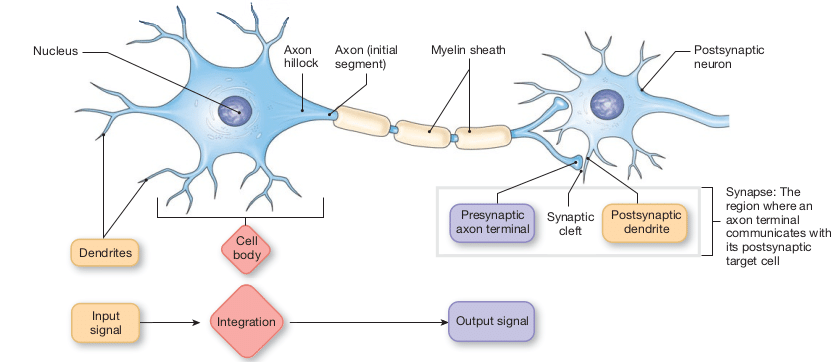
\includegraphics[width=\textwidth]{Figures/chapter_ne/biological_neuron.png} % Include the figure image
	\caption{Simplified illustration of neuron anatomy (\cite{neuron_model})}
	\label{fig:ne_biological_neuron} % Unique label used for referencing the figure in-text
\end{figure}

\parbreak\noindent These neurons communicate through electrical signals by mean of impulses (aka signal) in the cell wall. The impulses are mediated through the junctions called \textit{synapses} which are located on branches of the cell known as \textit{dendrites} (\cite{gurney2018introduction}). The neurons in turn are interconnected with many other neurons which are sending and receiving a multitude of incoming signals simultaneously. The signals are summed together in some way, but unlike in artificial models, where this is often a simple amplitude-based threshold, biological neurons rely heavily on the frequency of incoming spikes to determine firing. If the combined input (weighted by timing and firing rate) exceeds the neuron's threshold, it generates a voltage response (and thereby \textit{"fire"}) (\cite{gurney2018introduction}). The \text{synapse} is categorized as either being an excitory synapse which encourages the subsequent neuron from firing, or it can be an inhibitory synapse which discourages the subsequent neuron from firing (\cite{bishop1994neural}). Whether the \textit{synapse} is excitory or inhibitory is dictated by its strength (or weight). Provided that the neuron is \textit{"fired"}, a signal is sent to other neurons via the \textit{axon} and serve as input to the subsequent neuron (\cite{gurney2018introduction}).

\subsubsection{The Artificial Neuron}
\noindent At their core, neural networks are computational systems that consist of interconnected nodes that mimic the biological neuron seen in Figure \ref{fig:ne_biological_neuron}. Akin to the biological neural system, an artificial neuron is depicted in Figure \ref{fig:ne_artificial_neuron}. 

\parbreak
\begin{figure}[H] % Use [H] to suppress floating and place the figure/table exactly where it is specified in the text
	\centering % Horizontally center the figure on the page
	\includesvg[width=\textwidth]{Figures/chapter_ne/ne_artificial_neuron.svg} % Include the figure image
	\caption{Perceptron (Artificial Neuron) model (adapted from \cite{russell2016artificial})}
	\label{fig:ne_artificial_neuron} % Unique label used for referencing the figure in-text
\end{figure}

\parbreak\noindent The weighted sum (transfer function) depicted in Figure \ref{fig:ne_artificial_neuron} can be represented mathematically as follows (adapted from \cite{suzuki2011artificial}):
\begin{ceqn}
    \begin{equation}\label{alg:osum}
        O_{transfer\_function} = \sum_{i = 1}^{n}w_{ij}x_{i}+b
    \end{equation}
\end{ceqn}

\noindent where:
\begin{itemize}
    \item $x_{i}$ is the input signal
    \item $w_{ij}$ is the weight of the neuron
    \item $b$ is the bias
    \item $O_{transfer\_function}$ is weighted sum/transfer function result
\end{itemize}

\parbreak
\begin{figure}[H] % Use [H] to suppress floating and place the figure/table exactly where it is specified in the text
    \centering % Horizontally center the figure on the page
    \includesvg[width=\textwidth]{Figures/chapter_ne/ne_simple_neural_network.svg} % Include the figure image
    \caption{Simple Artificial Neural Network (adapted from \cite{nielsen2015neural})}
    \label{fig:ne_simple_neural_network} % Unique label used for referencing the figure in-text
\end{figure}

\parbreak\noindent The perceptron computes a weighted sum of its inputs plus a bias term. This bias acts like an adjustable threshold, shifting the activation left or right to ensure the neuron can fire even when input signals are weak or zero. Without the bias, the decision boundary (e.g., for classification) would always pass through the origin, severely limiting the network's flexibility (\cite{importance_of_bias}). Once the weighted sum plus the bias is calculated, an activation function is applied as follows (adapted from \cite{suzuki2011artificial}):
\begin{ceqn}
    \begin{equation}
        O_j = \phi(O_{transfer\_function})
    \end{equation}
\end{ceqn}

\noindent where $\phi$ is the activation function and $O_{transfer\_function}$ is the result from equation \ref{alg:osum}. These neurons, similiar to the biological neuron are interconnected with other neurons that receive and forward signals. Depicted in Figure \ref{fig:ne_simple_neural_network} is the general structure of a layered artificial neural network.

\parbreak\noindent A neural network is made up of 3 distinct layers, namely, the input layer, hidden layer, and output layer as shown in Figure \ref{fig:ne_simple_neural_network} (\cite{nielsen2015neural}). To explain by example, suppose we want to create a neural network to solve the simple XOR problem, that is, given certain bit value combinations, it returns a particular output according to the following truth table:

\parbreak
\begin{table}[H]
    \caption{The XOR problem truth table}
    \label{tab:xor_truth_table}
    \centering
    \begin{tabular}{|c|c|c|}
    \hline
    \textbf{Input A} & \textbf{Input B} & {\color[HTML]{BB5251} \textbf{Output}} \\ \hline
    0                & 0                & {\color[HTML]{BB5251} 0}               \\ \hline
    0                & 1                & {\color[HTML]{BB5251} 1}               \\ \hline
    1                & 0                & {\color[HTML]{BB5251} 1}               \\ \hline
    1                & 1                & {\color[HTML]{BB5251} 0}               \\ \hline
    \end{tabular}
\end{table}

\parbreak\noindent According to the truth table, there are two inputs which corresponds to two input neurons, and likewise, there is one output corresponding to one output neuron. Figure \ref{fig:ne_xor_network} illustrates what this network would look like. While mapping of the input and output layers are often simple, the hidden layers can be designed of arbitrary size and can be multilayered (\cite{nielsen2015neural}). The XOR problem highlights a fundamental limitation of single-layer perceptrons. While a single perceptron can model linearly separable functions like AND and OR, it cannot represent XOR, a non-linear problem where inputs must be classified based on their parity. This happens because no straight line can separate XOR's truth table outputs, however, this limitation is overcome by multi-layer perceptron (MLP) networks, where hidden layers enable non-linear decision boundaries through successive transformations. Researchers have developed numerous heuristics in order to design what the hidden layers should look like - these heuristics for example can help determine what the trade-off is for the number of hidden layers given the amount of training needed for the network while some researchers even argue that three hidden layers are enough to achieve exponential convergence and mitigate the problem of dimensionality (\cite{nielsen2015neural}, \cite{shen2021neural}).

\parbreak
\begin{figure}[H] % Use [H] to suppress floating and place the figure/table exactly where it is specified in the text
    \centering % Horizontally center the figure on the page
    \includesvg[width=\textwidth]{Figures/chapter_ne/ne_xor_network.svg} % Include the figure image
    \caption{XOR Problem Neural Network}
    \label{fig:ne_xor_network} % Unique label used for referencing the figure in-text
\end{figure}

\parbreak\noindent Once the neural network structure has been designed, weights are associate with each connection between neurons. To test what output results from a corresponding set of inputs, these inputs are fed into the input layer. The weighted sum of each neuron is calculated in the hidden layer and subjected to an activation function. This is then fed forward as input into the output layer which in response, again, calculates the weighted sum and applied to an activation function producing a final output. This flow of information from the input to the output characterizes the network as a feedforward neural network which essentially means there are no loops within the network (\cite{nielsen2015neural}). Neural networks that have loops form part of other distinct models, one of which is recurrent neural networks (RNNs).

\subsection{The Activation Function}
The activation function controls whether the neuron \textit{"fires"}, using amplitude-based thresholds to make this decision. Unlike biological neurons that rely on firing frequency, this artificial approach provides a way to introduce non-linearity into the network. If an activation function is not used in a neural network, the output signal will always be a linear function that is a polynomial of degree one (\cite{sharma2017activation}). There are three classes of activation to choose from depending on the problem at hand, namely, a step function, linear function, and non-linear function (\cite{suzuki2011artificial}). To give an overview of the most popular activation functions:

\parbreak\noindent \textbf{Binary Step Function} (\textit{Step Function Category}): This is the simplest activation function that either outputs a 0 or 1 depending on whether some threshold is met. It is mathematically represented as shown in Equation \ref{alg:binary_step_function} and visually illustrated in Figure \ref{fig:ne_binary_step_plot} (\cite{sharma2017activation}). Binary step functions are typically used when creating binary classifiers as the output maps directly to two options (\cite{sharma2017activation}).
    
\parbreak
\begin{ceqn}
    \begin{equation}\label{alg:binary_step_function}
        f(x) = 
        \begin{cases} 
            1 \:\: if \:\: x \geq 0 \\
            0 \:\: if \:\: x < 0 
        \end{cases}
    \end{equation}
\end{ceqn}

\begin{figure}[H] % Use [H] to suppress floating and place the figure/table exactly where it is specified in the text
    \centering % Horizontally center the figure on the page
    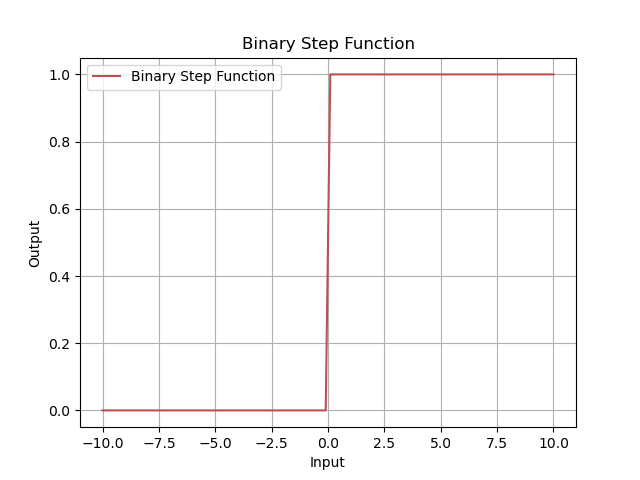
\includegraphics[width=\textwidth]{Figures/chapter_ne/ne_binary_step_plot.png} % Include the figure image
    \caption{Binary Step Activation Function Plot}
    \label{fig:ne_binary_step_plot} % Unique label used for referencing the figure in-text
\end{figure}

\parbreak\noindent \textbf{Linear Activation Function} (\textit{Linear Function Category}): This function represents a relationship that is directly proportional to the input. It is mathematically represented as shown in Equation \ref{alg:linear_function} and visually illustrated in Figure \ref{fig:ne_linear_plot} (\cite{sharma2017activation}). Linear activation functions are best suited for regression problems where linear relationships are the only concern (\cite{sharma2017activation}).
  
\begin{ceqn}
    \begin{equation}\label{alg:linear_function}
        f(x) = ax
    \end{equation}
\end{ceqn}

\parbreak
\begin{figure}[H] % Use [H] to suppress floating and place the figure/table exactly where it is specified in the text
    \centering % Horizontally center the figure on the page
     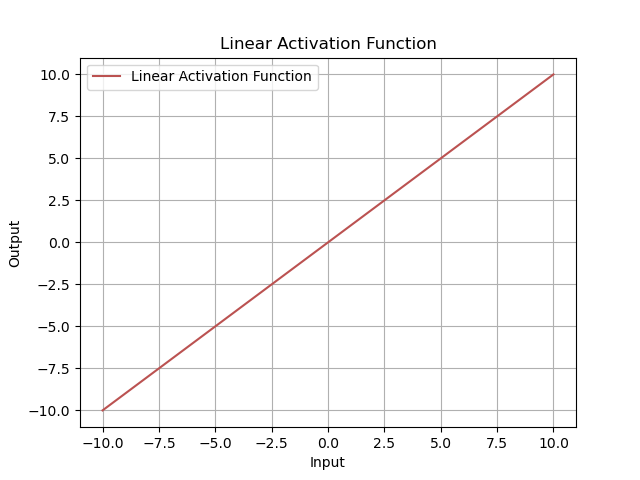
\includegraphics[width=\textwidth]{Figures/chapter_ne/ne_linear_plot.png} % Include the figure image
    \caption{Linear Activation Function Plot}
    \label{fig:ne_linear_plot} % Unique label used for referencing the figure in-text
\end{figure}

\parbreak\noindent \textbf{Sigmoid Activation Function} (\textit{Non-linear Function Category}): This function is the most widely used activation function due to its ability to be continuously differentiable and non-symmetric about zero meaning that the sign of all output values of neurons will be the same (\cite{sharma2017activation}). It is mathematically represented as shown in Equation \ref{alg:sigmoid_function} and visually illustrated in Figure \ref{fig:ne_sigmoid_plot} (\cite{sharma2017activation}). This activation function brings non-linearity into the neural network having applicability a wide range of tasks such as classification problems, function approximation, etc - essentially problems that involve complex relationships to be learned (\cite{sharma2017activation}).
    
\begin{ceqn}
    \begin{equation}\label{alg:sigmoid_function}
        f(x) = \frac{1}{e^{-x}}
    \end{equation}
\end{ceqn}

\parbreak
\begin{figure}[H] % Use [H] to suppress floating and place the figure/table exactly where it is specified in the text
    \centering % Horizontally center the figure on the page
    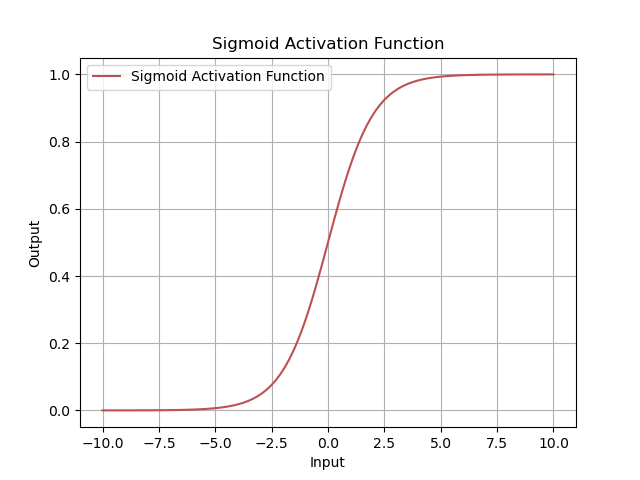
\includegraphics[width=\textwidth]{Figures/chapter_ne/ne_sigmoid_plot.png} % Include the figure image
    \caption{Sigmoid Activation Function Plot}
    \label{fig:ne_sigmoid_plot} % Unique label used for referencing the figure in-text
\end{figure}

\noindent There are many other popular activation functions that include \textit{ReLU}, \textit{LeakyReLU}, \textit{Hyperbolic Tangent}, and so on which each have their applicability in a particular task. Choosing the correct activation function has many considerations such as the number of hidden layers in the network, the training method used, hyperparameter tuning, etc. (\cite{sharma2017activation}).

\subsection{Backpropagation}
Backpropagation, short for backward propagation of errors, is a fundamental algorithm that is used to train neural networks. Traditionally in early years of artificial neural network research (1950s-1980s), the training of neural networks was not common and made the use of neural networks undesirable (\cite{aggarwal2018neural}). Since its introduction in the 1980s, backpropagation has become a cornerstone of modern deep learning (\cite{aggarwal2018neural}).

\parbreak\noindent Backpropagation's main concept is based on understand how changing the weights and biases in a network impacts the cost function (\cite{nielsen2015neural}). The cost function measures the network's overall performance across all training examples, serving as the optimisation target during learning. This differs from the loss function, which calculates the error for a single sample. The cost function aggregates these individual losses (typically through averaging) to guide weight adjustments across the entire dataset. The cost function is defined mathematically as (\cite{nielsen2015neural}):
\begin{ceqn}
    \begin{equation}\label{alg:cost_function}
        C = \frac{1}{2n}\sum_{x} ||y(x)-a^L(x)||^2
    \end{equation}
\end{ceqn}

\noindent where:
\begin{itemize}
    \item $n$ is the total number of training examples
    \item $x$ is the training individual example
    \item $y(x)$ is the desired output
    \item $a^L(x)$ is the vector of activation outputs when $x$ is the input
\end{itemize}

\parbreak\noindent There are four main equations that are needed for backpropagation to work (\cite{nielsen2015neural}):

\begin{enumerate}
    \item The first equation allows the computation of the error in output layer $L$:
    \begin{ceqn}
        \begin{equation}\label{alg:bp1}
            \delta^L = \nabla_aC\odot\sigma'(z^L)
        \end{equation}
    \end{ceqn}
    \noindent where:
    \begin{itemize}
         \item $\delta^L$ is the error in output layer $L$
        \item $\nabla_aC$ is a vector whose components are the partial derivatives $\frac{\partial C}{\partial a_j^L}$ - in other words, the rate of change of C with   respect to the output activation
        \item $\odot$ is the elementwise multiplication operator
        \item $\sigma'(z_J^L)$ measures how fast the activation function $\sigma$ changes at $z_j^L$
        \item $z_j^l$ is the weighted input of neuron $j$ at layer $l$
    \end{itemize}

    \item The second equation allows the computation of the error $\delta^l$ in terms of the error in the following layer:
    \begin{ceqn}
        \begin{equation}\label{alg:bp2}
            \delta^l = ((w^{l+1})^T\delta^{l+1})\odot\sigma'(z^l)
        \end{equation}
    \end{ceqn}
    \noindent where:
    \begin{itemize}
        \item $\delta^l$ is the error in the next layer
        \item $(w^{l+1})^T$ is the transpose of the weight matric $w^{l+1}$ for the $(1+l)$-th layer
    \end{itemize}

    \item Equation \ref{alg:bp1} and \ref{alg:bp2} can be combined to provide the third main equation of backpropagation which allows the computation of the error $\delta^l$ for any layer in the network:
    \begin{ceqn}
        \begin{equation}\label{alg:bp3}
            \frac{\partial C}{\partial b_j^l} = \delta_j^l
        \end{equation}
    \end{ceqn}

    \item The fourth and final equation allows the computation of partial derivatives $\frac{\partial C}{\partial w_{jk}^l}$ in terms of $\delta^l$ and $a^{l-1}$:
    \begin{ceqn}
        \begin{equation}\label{alg:bp4}
            \frac{\partial C}{\partial w_{jk}^l} = a_k^{l-1}\delta_j^l
        \end{equation}
    \end{ceqn}
\end{enumerate}

\parbreak\noindent With the above four main equations in mind, the backpropagation algorithm works as follows:

\begin{algorithm}[H]
	\caption{Basic Backpropagation Algorithm (\cite{nielsen2015neural})}\label{alg:backpropogation_algorithm}
	\begin{algorithmic}[1]
    \item \textbf{Input} value x: Set the corresponding activation $a^1$ for the input layer
    \item \textbf{Feedforward}: For each layer, $l=1,2,3,...,L$, compute the weighted sum $z^l=w^la^{l-1}+b^l$ and the activation value $a^l=\sigma(z_l)$
	\item \textbf{Output error} $\delta^L$: Compute the error of the output layer using $\delta^L=\nabla_aC\odot\sigma'(z^L)$ (Equation \ref{alg:bp1})
	\item \textbf{Backpropagate the error}: For each layer, $l=L-1, L-2,...,2$, computer the error for that layer using $\delta^l=((w^{l+1})^T\delta^{l+1}) \odot\sigma'(z^l)$ (Equation \ref{alg:bp2})
	\item \textbf{Output}: The gradient of the cost function is given by $\frac{\partial C}{\partial b_j^l} = \delta_j^l$ and $\frac{\partial C}{\partial w_{jk}^l} = a_k^{l-1}\delta_j^l$ (Equation \ref{alg:bp3} and \ref{alg:bp4} respectively)
\end{algorithmic}
\end{algorithm}

\parbreak\noindent In essence, the backpropogation algorithm computes the gradient of the loss function with respect to each weight in the network for a single training example, however, calculating these gradients alone does not update the network. To actually train the model, backpropagation is typically combined with an optimisation algorithm such as stochastic gradient descent (SGD). Gradient descent uses the computed gradients to iteratively adjusts the weights in a direction that minimises the overall cost function. In the case of SGD, this process is performed using small batches or individual training examples, which allows for faster and more scalable learning. This combination of backpropagation and gradient descent forms the foundation of most conventional neural network training mechanisms (\cite{nielsen2015neural}).

\section{Neural Architecture Search}\label{sec:ne_nas}
Neural Architecture Search (NAS) is a technique in artificial intelligence aimed at automating the design of neural network architectures as opposed to the traditional method of crafting these neural networks by hand and through trial-and-error, both of which are time-consuming and prone to suboptimal outcomes (\cite{ren2021comprehensive}). NAS addresses these challenges by employing algorithms to discover optimal or near-optimal architectures tailored for a specific task. NAS represents a significant shift towards making machine learning more scalable and accessible, bridging the gap between model development and deployment (\cite{elsken2019neural}).

\parbreak\noindent NAS is based on three core components and are combined to form the NAS methods illustrated in Figure \ref{fig:ne_nas}. (\cite{elsken2019neural}):

\begin{itemize}
    \item \textbf{Search Space}: This component defines the set of possible neural network architectures that NAS can explore and includes various design elements such as layer types, number of layers, connectivity patterns, and the neural networks hyperparameters. A well-structured search space is extremely important as it balances between being expressive enough to capture high-performing architectures while still being constrained enough to allow efficient exploration (\cite{elsken2019neural}).
    \item \textbf{Search strategy}: This component dictates how the NAS algorithm navigates the search space to identify optimal architectures. Common search strategies include reinforcement learning, evolutionary algorithms, and gradient-descent methods (\cite{liu2021survey}). Reinforcement learning makes use of a controller model to generate architectural decisions, while evolutionary algorithms mimic natural selection by evolving a population of candidate architecture solutions over successive generations. Gradient-based approaches, such as Differentiable Architecture Search (DARTS), enable more efficient exploration by allowing continuous relaxation of the search space (\cite{liu2021survey}).
    \item \textbf{Performance Estimation Strategy}: This component assesses how promising a candidate architecture is without fully training it, which is essential due to the high computation cost involved in evaluating each neural network design (\cite{elsken2019neural}). Techniques like early stopping, weight sharing, and surrogate models are used to estimate performance more efficiently (\cite{elsken2019neural}).
\end{itemize}

\parbreak
\begin{figure}[H] % Use [H] to suppress floating and place the figure/table exactly where it is specified in the text
	\centering % Horizontally center the figure on the page
	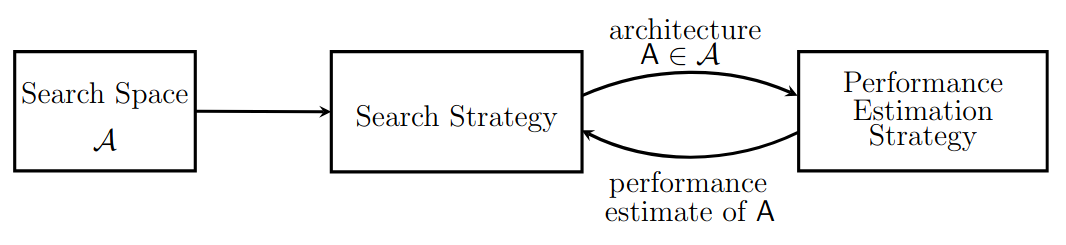
\includegraphics[width=\textwidth]{Figures/chapter_ne/ne_nas.png} % Include the figure image
	\caption{Neural Architecture Search methods framework (\cite{elsken2019neural})}
	\label{fig:ne_nas} % Unique label used for referencing the figure in-text
\end{figure}

\parbreak\noindent NAS has evolved through the development of many methods, each offering distinct approaches in navigating the search space. One prominent approach is \textbf{reinforcement learning-based} learning, where the generation of a neural network architecture is considered an agent's action and the agent's reward correlated to the performance of a trained architecture on unseen data (\cite{elsken2019neural}). The most influential method is \textbf{evolutionary algorithms} (mentioned in Chapter \ref{chapter_ea}) which mimics biological evolution by iteratively apply genetic operators and selecting high-performing architectures. This approach is highly adaptive however can also become computationally intensive fast. More recently, \textbf{gradient-based} NAS methods as mentioned previously have gained popularity for their efficiency. DARTS for example, relaxes the discrete search space into a continuous one enabling gradient descent optimization to find optimal architectures far quicker and with reduced computational demands (\cite{liu2021survey}). These methods differ in scalability, model performance, and efficiently. Reinforcement learning and evolutionary algorithms excel in finding innovative architectures but are computationally expensive while gradient-based approaches offer faster and more resource-efficient search offering more practical application, however, do not innovate as well (\cite{elsken2019neural}).

\parbreak\noindent Despite the promising potential that NAS provides, it still faces several significant challenges. The most pressing issue is its high computational cost (\cite{liu2021survey}). Traditional NAS methods, especially those making use of reinforcement learning and evolutionary algorithms require the training of thousands of candidate models, consuming computational resources and time exponentially, making NAS undesirable to researchers and organizations with limited infrastructure (\cite{elsken2019neural}). Another issue lies in the design of the search space. Creating a search space that is both expressive and efficient becomes a complex task. A poorly designed search space can either be to restrictive hindering exploration, or too expensive leading to inefficient searches and suboptimal models (\cite{liu2021survey}).

\parbreak\noindent Recent advancements in NAS have focused on mitigating the challenge of computational demands and improving generalization. One notable development is the use of weight sharing whereby multiple candidate solution architectures share parameters during training. This technique significantly reduces the time needed to train each model therapy cutting computational demands (\cite{pham2018efficient}). Another advancement in the field of NAS is the aforementioned DARTS technique which transforms the discrete search space in a continuous one, allowing for architecture parameters to be optimized efficiently using gradient descent based methods and thereby enhancing the search speed and reducing resource consumption (\cite{liu2021survey}). Additionally, strategies like proxy models and early stopping have been employed to estimate model performance without fully training each candidate solution architecture, helping mitigate excessive computation while still allowing for the consideration of innovative architectures (\cite{liu2021survey}). NAS has also extended into real-world application such as computer vision whereby NAS-designed models have achieved state-of-the-art results in image classification and object detection. In natural language processing, NAS has contributed to more efficient transformer architectures, optimizing performance for tasks such as text generation and machine translation (\cite{elsken2019neural}).


\section{Neuroevolution of Augmenting Topologies}\label{sec:ne_neat}
\subsection{Introduction to NEAT}
The Neuroevolution of Augmenting Topologies (NEAT) algorithm is a pioneering method in neuroevolution, known for its powerful ability evolve both the structure and weights of a neural network (\cite{stanley2019designing}). NEAT begins with simple networks and gradually increases its complexity through evolutionary principles. It is based on three core principles in an attempt to solve the challenges that topology and weight evolving artificial neural networks (TWEANNs) face, namely, (1) its unique genetic encoding scheme, (2) mechanism of speciation, and (3) minimization of dimensionality through incremental growth from minimal structures (\cite{stanley2002evolving}).

\parbreak
\begin{figure}[H] % Use [H] to suppress floating and place the figure/table exactly where it is specified in the text
	\centering % Horizontally center the figure on the page
	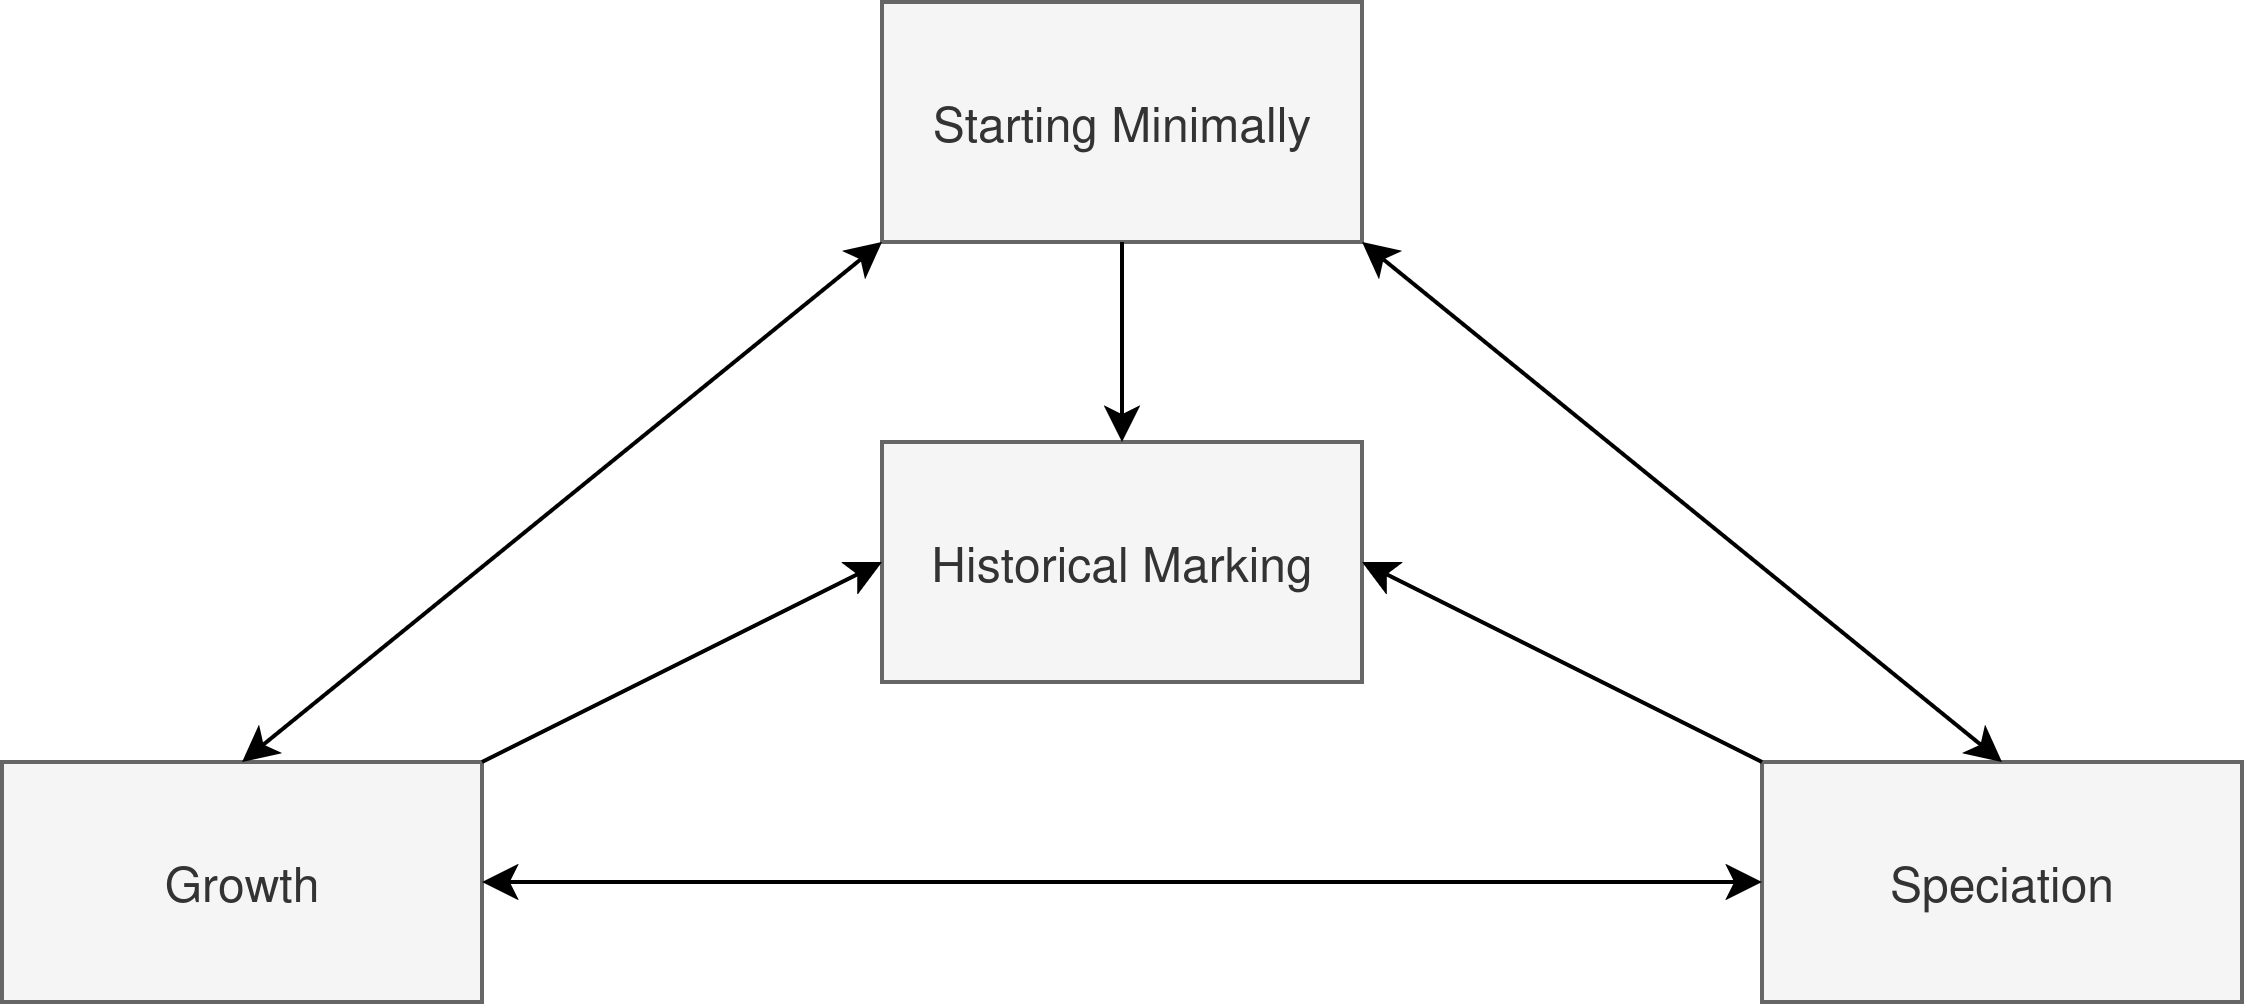
\includegraphics[width=\textwidth]{Figures/chapter_ne/ne_neat_components.png} % Include the figure image
	\caption{NEAT Component Dependencies (adapted from \cite{stanley2002evolving})}
	\label{fig:neat_depedencies} % Unique label used for referencing the figure in-text
\end{figure}

\parbreak\noindent Genetic encoding allows the transformation between phenotype, being the actual neural network representation, to genotype, being a linear string subject to genetic operators. Mutations to these genotypes introduce changes such as the addition of new nodes, altered weights, or additional connections, while crossover operations combine features from parent neural networks. These genetic operations are tailored in such away that functional integrity is maintained, ensuring that the offspring networks inherit the best traits. Importantly, NEAT aims to solve the issue of competing conventions whereby candidate solutions can possibly represent the same outcome even though they have different gene configurations. With reference to Figure \ref{fig:competing_convension}, the crossover between two neural networks that are identical representations but are just different structure configurations can lead to a loss in information (\cite{stanley2002evolving}). This challenge stems from the isomorphism problem, where functionally equivalent networks may have different node and connection patterns, making meaningful genetic recombination difficult.

\parbreak
\begin{figure}[H] % Use [H] to suppress floating and place the figure/table exactly where it is specified in the text
	\centering % Horizontally center the figure on the page
	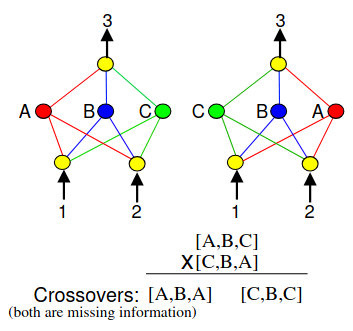
\includegraphics[width=\textwidth]{Figures/chapter_ne/ne_competing_convention.png} % Include the figure image
	\caption{Competing Convention between Neural Network Solutions (adapted from \cite{stanley2002evolving})}
	\label{fig:competing_convension} % Unique label used for referencing the figure in-text
\end{figure}

\parbreak\noindent Speciation preserves unique structures by grouping similar networks into species, protecting novel characteristics from premature elimination. This mechanism prevents innovative offspring from being directly compared with established and well performing networks, which might otherwise out compete them prematurely. By fostering innovation within smaller networks, speciation allows NEAT to better exploit the search space and void stagnation (\cite{stanley2002evolving}). While speciation mechanisms exist across evolutionary algorithms (as mentioned in Chapter \ref{chapter_ea}), NEAT implements this through its distinctive approach of historical markings and compatibility distance, which constitutes its key innovation.

\parbreak\noindent Incremental growth refers to the gradual introduction of nodes and connections through subsequent generations, enabling networks to evolve complexity only when advantageous. This approach avoids computational overhead when dealing with unnecessarily complex networks in early stages and ensures that the algorithm uses these networks as core building blocks in creating innovative candidate solutions (\cite{stanley2002evolving}).

\subsection{Mechanics of NEAT}
\subsubsection{Initialisation of Population}
The mechanics of NEAT rely on sophisticated yet efficient process that balance exploration and exploitation in evolving neural networks. The algorithm begins with a population of minimal neural networks, typically consisting of input and output nodes without hidden layers. This simplicity is intentional, as NEAT focuses on incremental growth by introducing new nodes and connection only when they enhance the networks performance. The reason being is that networks that are randomly generated and complex tend to go through the effort of removing connections and nodes that are not needed in the first place (\cite{stanley2002evolving}). NEAT's initialisation scheme prevents modifications where fitness functions track network size, as this would unnecessarily complicate fitness evaluation. Starting out minimally ensures that candidate solutions explore the search space in the lowest dimensional weight space first, resulting in dramatic performance gains early on. Another added advantage of starting out simply is the manifestation of speciation. Starting out simply and complexifying over subsequent generations aligns with Darwinian principles (\cite{stanley2002evolving}).

\subsubsection{Phenotype-Genotype Mapping}
NEAT's genetic encoding scheme is designed in such away that allows genetic operations to be performed without leading to non-functional neural networks, a problem that traditional TWEANNs face. The neural network (phenotype) is encoded in a linear representation as shown in Figure \ref{fig:genotype_phenotype_neat_mapping}.

\parbreak
\begin{figure}[H] % Use [H] to suppress floating and place the figure/table exactly where it is specified in the text
	\centering % Horizontally center the figure on the page
	\includesvg[width=\textwidth]{Figures/chapter_ne/ne_genotype_mapping.svg} % Include the figure image
	\caption{NEAT's Genotype-Phenotype Mapping (adapted from \cite{stanley2002evolving})}
	\label{fig:genotype_phenotype_neat_mapping} % Unique label used for referencing the figure in-text
\end{figure}

\parbreak\noindent The mapping works by assigning each node in the neural network representation with an index. The genome of the genotype representation is made up of \textit{node genes} and \textit{connection genes}. Node genes represents input, hidden, and output nodes that make up the network whereas connection genes specify the following information:

\begin{itemize}
    \item \textbf{In}: The outgoing connection of the node.
    \item \textbf{Out}: The incoming connection of the node.
    \item \textbf{Weight}: The weight of the connection.
    \item \textbf{Enabled}: Dictates whether the connection is active or not.
    \item \textbf{Innov}: Serves as a historical marker in tracking corresponding genes.
\end{itemize}

\subsubsection{Genetic Operators}
\noindent NEAT makes use of both mutation and crossover to produce viable offspring. Mutation has the ability to change both the connection weights and network structures. Weight mutation works as normal in any evolutionary algorithm whereby the mutation value is chosen and changed according to some function as explained in Section \ref{label:ea_genetic_operators}. Structural mutations can occur in two ways, each of which expands the size of the genome (\cite{stanley2002evolving}):
\begin{itemize}
    \item \textbf{Add connection} mutation: This mutation adds a single new connection between two previously unconnected nodes. Figure \ref{fig:neat_add_connection} illustrates this by mutating the genome such that a connection is formed between node 1 and 4.
    \item \textbf{Add node} mutation: This mutation splits an existing connection and places a new node where this existing connection use to be. This involves the old connection being disabled. The new connection leading from the old node into the new node receives a weight of 1 while the new connection leading from the new into the other old node receives the same weight as the old connection. Figure \ref{fig:neat_add_node} illustrates this by mutating the genome such that node 6 is added, with two new connections forming between node 1 and 6, and node 6 and 5.
\end{itemize}

\parbreak\noindent This mutation mechanism allows the initial effect of mutation to be minimised. In traditional mutations as those seen in genetic programming which allows extraneous structures to be added, NEAT essentially forces the structures to be evolved in complex ways later on allowing the network to exploit simple structures first (\cite{stanley2002evolving}). The crossover genetic operator is applicable in NEAT as well, however, enabled through a mechanism known as gene tracking through historical markings.

\parbreak
\begin{figure}[H] % Use [H] to suppress floating and place the figure/table exactly where it is specified in the text
	\centering % Horizontally center the figure on the page
	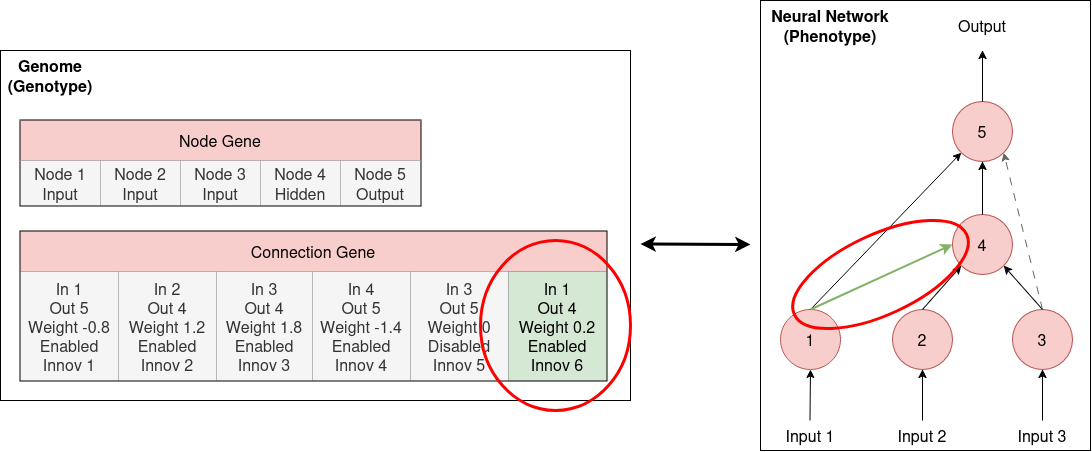
\includegraphics[width=\textwidth]{Figures/chapter_ne/ne_add_connection.png} % Include the figure image
	\caption{NEAT's Add Connection Mutation Mechanism (adapted from \cite{stanley2002evolving})}
	\label{fig:neat_add_connection} % Unique label used for referencing the figure in-text
\end{figure}

\parbreak
\begin{figure}[H] % Use [H] to suppress floating and place the figure/table exactly where it is specified in the text
	\centering % Horizontally center the figure on the page
	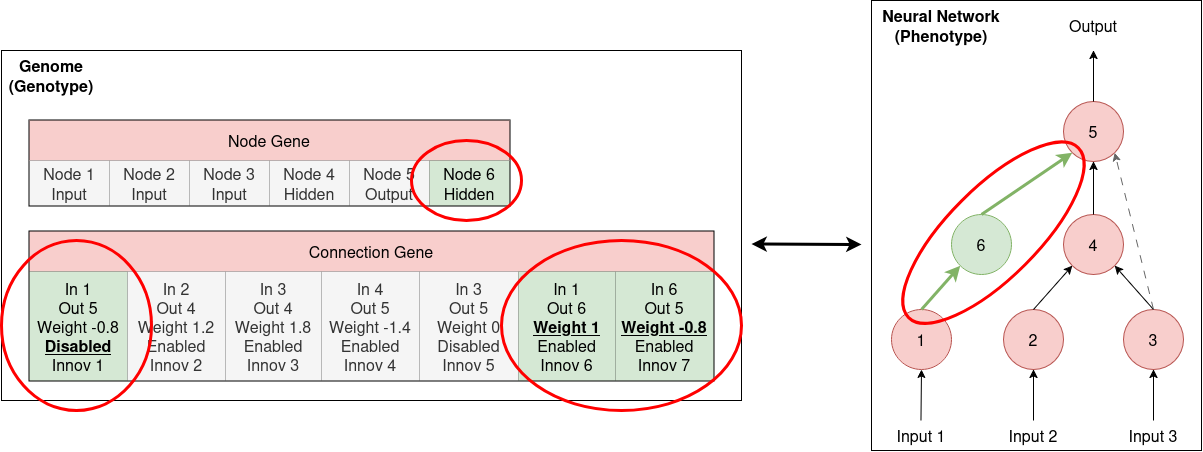
\includegraphics[width=\textwidth]{Figures/chapter_ne/ne_add_node.png} % Include the figure image
	\caption{NEAT's Add Node Mutation Mechanism (adapted from \cite{stanley2002evolving})}
	\label{fig:neat_add_node} % Unique label used for referencing the figure in-text
\end{figure}

\subsubsection{Historical Markings}
Historical markings is a powerful capability of NEAT that solves the problem of competing conventions. Innovation numbers that are seen in Figure \ref{fig:genotype_phenotype_neat_mapping} enables this capability and represents a chronology of the appearance of every gene. When the initial population is generated, a unique innovation number is assigned to every unique connection. When a new gene appears, a \textit{global innovation number} is incremented and assigned to that gene. 

\parbreak
\begin{figure}[H] % Use [H] to suppress floating and place the figure/table exactly where it is specified in the text
	\centering % Horizontally center the figure on the page
	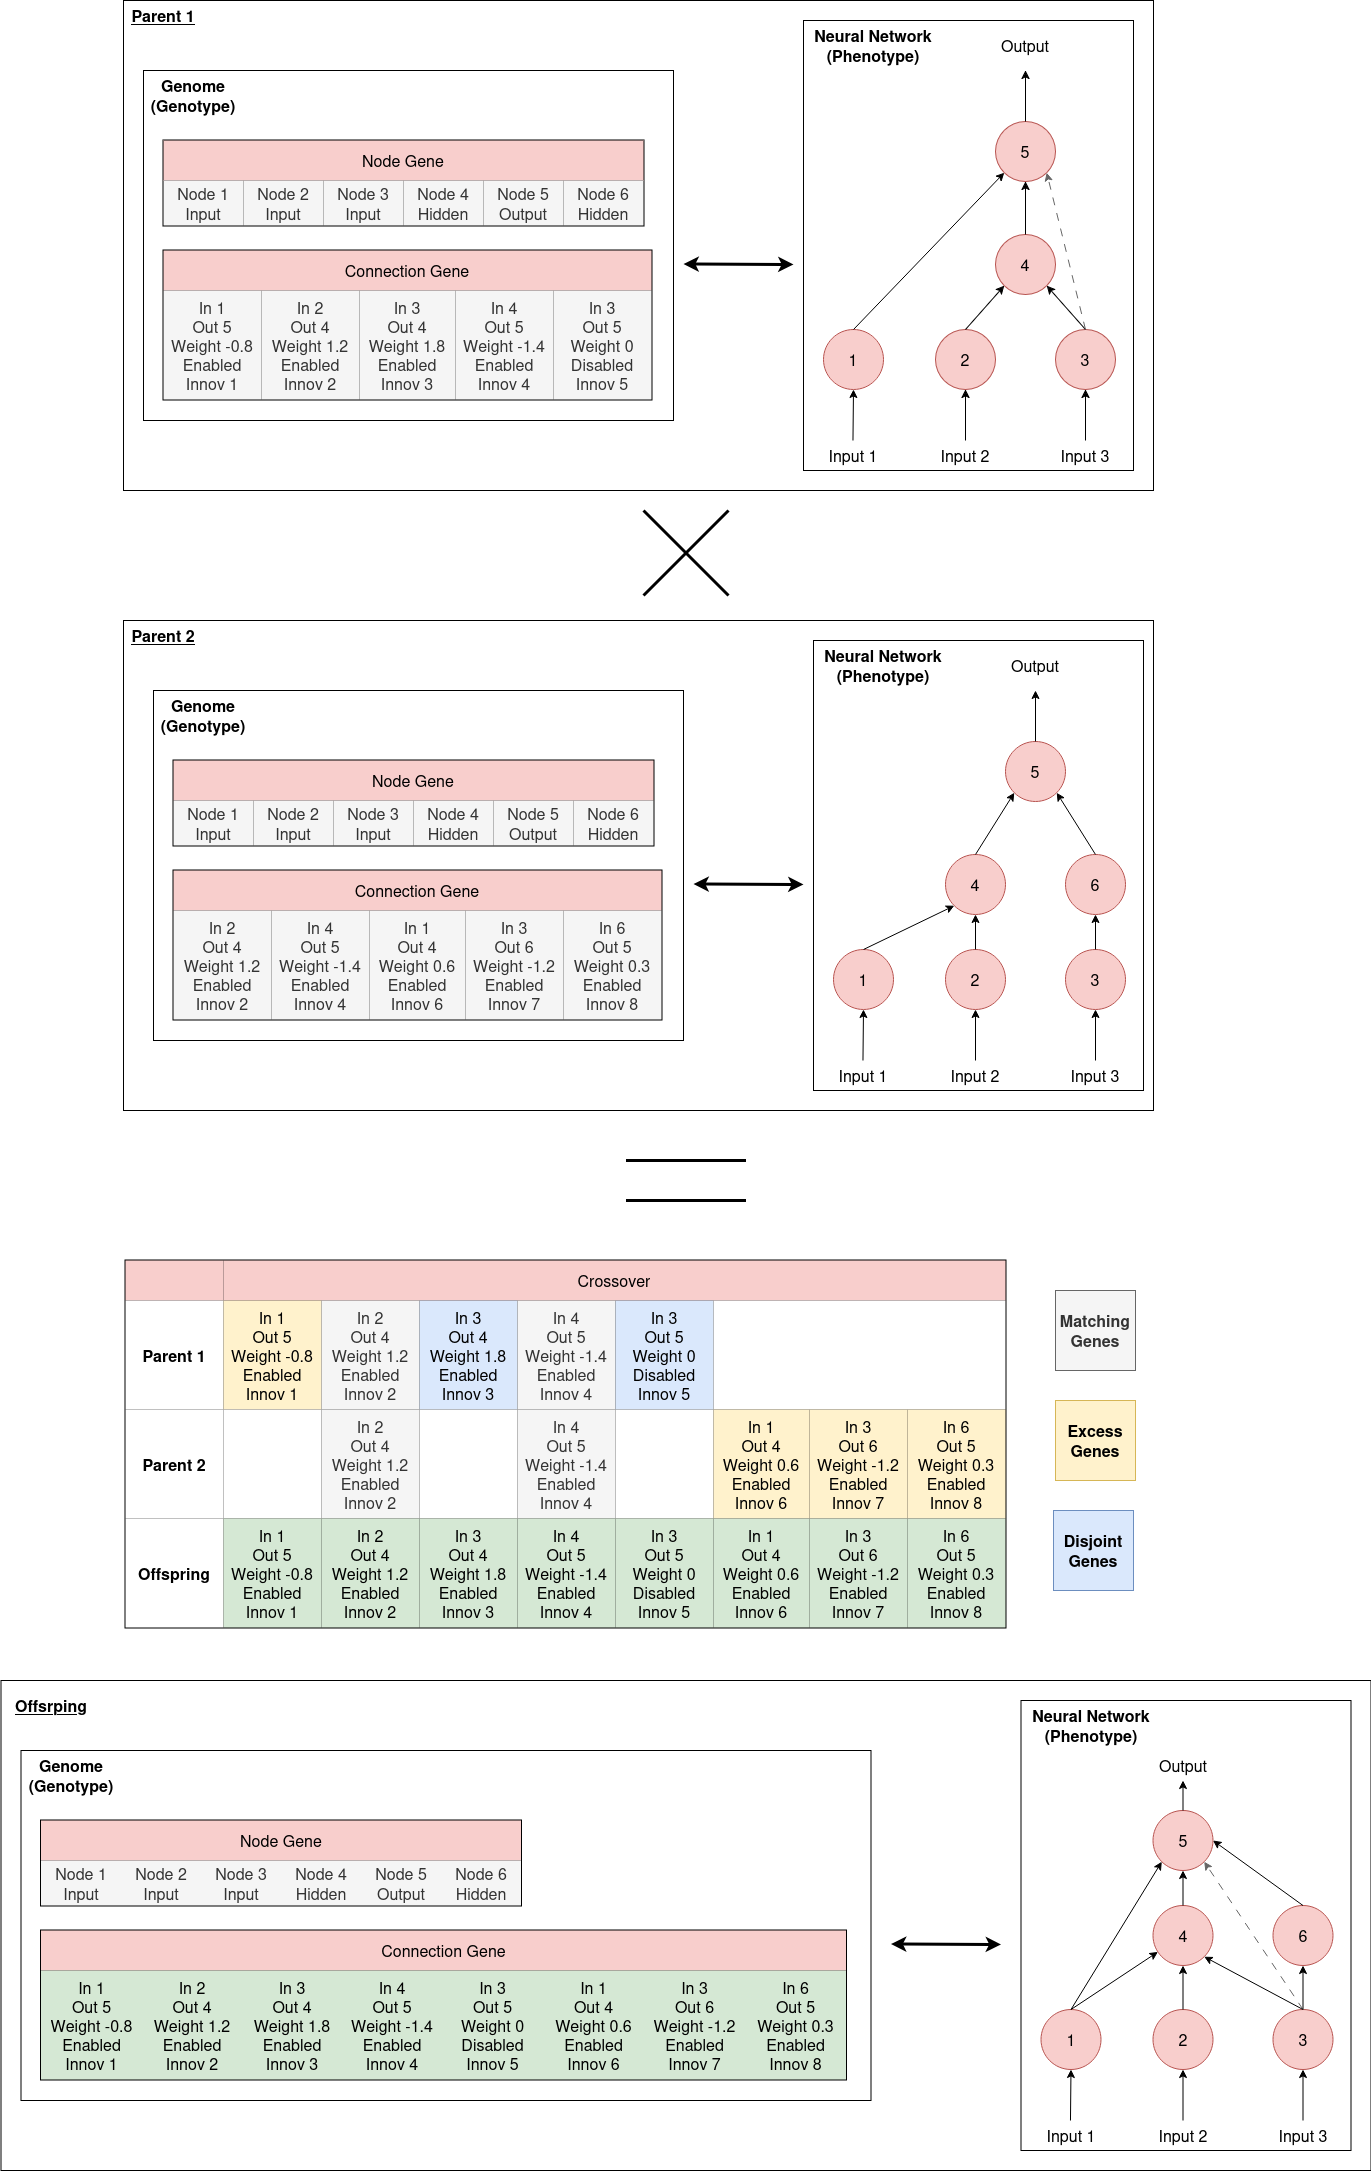
\includegraphics[width=\textwidth]{Figures/chapter_ne/ne_neat_crossover.png} % Include the figure image
	\caption{NEAT's Crossover Mechanism (adapted from \cite{stanley2002evolving})}
	\label{fig:neat_crossover} % Unique label used for referencing the figure in-text
\end{figure}

\parbreak\noindent There might be a chance mutations may result in the same structural innovation amongst multiple candidate solutions within a generation - to avoid assigning different innovation numbers in this scenario, a list of gene innovations are kept for that generation meaning that if mutations result in the same structural innovation amongst multiple genes, they receive the same innovation number.

\parbreak\noindent Importantly, tracking the historical markings of genes provides a way to exactly know which genes match up when performing crossover. Genes that line up according to their \textit{innovation number} are called \textit{matching} genes. Genes that do not split are categorized as either \textit{disjoint} or \textit{excess} depending what their positions are with regard to the other parent. For example, in Figure \ref{fig:neat_crossover}, gene 4 to 6 of parent 1, and gene 1 to 4 of parent 2 form disjoint genes while gene 7 to 8 of parent 2 form genes that are in excess. Matching genes up in this fashion using innovation allows crossover to happen naturally.

\subsubsection{Speciation}
Speciation was introduces in NEAT to allow candidate solutions to compete primarily within their own niches as opposed to the entire population. Doing this means that new topological innovations are protected in a new niche allowing them to optimize through competition within the niche. The idea behind this is to prevent premature convergence and stagnation allowing candidate solutions to exploit the search space thoroughly. Speciating is efficiently enabled through innovation numbers by comparing how many disjoint genes there are between candidate solutions. Essentially, the more disjoint two genomes are, the less historical markers they share and by that extent are less compatible (\cite{stanley2002evolving}). This compatibility can be calculated through the following mathematical equation (\cite{stanley2002evolving}):
\begin{ceqn}
    \begin{equation}\label{alg:speciation}
        \delta = \frac{c_1E}{N} + \frac{c_2D}{N} + c_3\cdot{\overline{W}}
    \end{equation}
\end{ceqn}

\noindent where:
\begin{itemize}
    \item $\delta$ is the compatibility distance between a pair of genomes
    \item $E$ is the number of excess genes
    \item $D$ is the number of disjoint genes
    \item $\overline{W}$ is the average weight difference of matching genes
    \item $N$ is the number of genes in the larger genome (serving as a normalization)
    \item $c_1$, $c_2$, and $c_3$ serve as adjustments in the importance of the three factors
\end{itemize}

\parbreak\noindent The compatibility distance, $\delta$, allows speciation using a threshold $\delta_t$. During the evolution process, a list of species is maintained, and candidate solutions are speciated in each generation. A species is represented by a random genome inside that species known as the \textit{species representative}. Given a genome $g$ in a generation, it is placed in the first species that it is found to be compatible within the species representative of that species - if no species is found, it forms part of a new species (\cite{stanley2002evolving}).

\parbreak\noindent Species have the benefit of having access to all candidate solution's fitness function values within that species during reproduction which is a mechanism known as \textit{explicit fitness sharing}. This means that a single candidate solution is unlikely to dominate the species. Speciation involves an adjusted fitness functions as follows (\cite{stanley2002evolving}):
\begin{ceqn}
    \begin{equation}\label{alg:speciation}
        f'_i = \frac{f_i}{\sum_{j=1}^{n}sh(\sigma(i,j))}
    \end{equation}
\end{ceqn}

\noindent where:
\begin{itemize}
    \item $f'_i$ is the fitness of candidate solution $i$
    \item $f_i$ is the chosen fitness function for the neural network
    \item $\sigma(i,j)$ is the compatibility distance seen in Equation \ref{alg:speciation} between organism $i$ and $j$
    \item $sh$ is the sharing function that operates as follows:
    \begin{ceqn}
        \begin{equation}\label{alg:sharing_function}
            sh(\sigma(i,j)) = 
            \begin{cases} 
                1 \:\: if \:\: \delta(i,j) > \delta_t \\
                0 \:\: otherwise
            \end{cases}
        \end{equation}
    \end{ceqn}

    \item $\sum_{j=1}^{n}sh(\sigma(i,j))$ reduces to the number of candidate solutions in the same species as candidate solution $i$
\end{itemize}

\parbreak\noindent Making use of this adjusted fitness function means that species reproduce by first eliminating the weakest links. Speciating the population in this regard ensures that the topological innovation is protected.

\subsubsection{Minimizing Dimensionality}
The last core concept in NEAT is its minimization in dimensionality through incremental growth from minimal structures. When initializing the population at the start of the algorithm, NEAT biases its search around minimal dimensional spaces by initializing candidate solutions with zero hidden nodes. As subsequent generations occur, new structures are introduced incrementally by means of mutation and crossover. This means that the topology innovations that occur are justified. Due to starting out minimally, NEAT outperforms other TWEANN based search algorithms requiring fewer dimension to find optimal solutions (\cite{stanley2002evolving}).

\subsection{Strengths and Challenges of NEAT}
The NEAT algorithm has several strengths that have contributed to its widespread use in artificial intelligence research. One of its primary advantages is its efficiency in evolving neural network with minimal complexity. When applied to the double pole balancing problem, NEAT was able to find an optimal solution in as little as 24 generations made up of 150 nodes, a network far more minimal than other traditional TWEANNs (\cite{stanley2002evolving}). By starting out with simple networks and adding complexity gradually, NEAT avoids the inefficiencies associated with random initialisation of large, complex networks. This makes NEAT particularly suitable for tasks where the optimal topology is unknown.

\parbreak\noindent Another strength of NEAT is its ability to preserve diversity within the population by means of its speciation algorithm which ensures that innovative solutions are no prematurely discarded, allowing the algorithm to explore a wide range of architectures. In the original paper of NEAT, to understand the importance of speciation, a graph was produced to illustrate how speciation impacts innovation which is shown in Figure \ref{fig:neat_speciate_vis}. As subsequent generations occur, species guide their search collectively towards an optimal solution showcasing its thorough search capability. Fitness sharing within species also prevents over-optimization of a single solution thereby fostering more robust search process. These features make NEAT well-suited for solving complex and high-dimensional problems (\cite{stanley2002evolving}). 

\parbreak
\begin{figure}[H] % Use [H] to suppress floating and place the figure/table exactly where it is specified in the text
	\centering % Horizontally center the figure on the page
	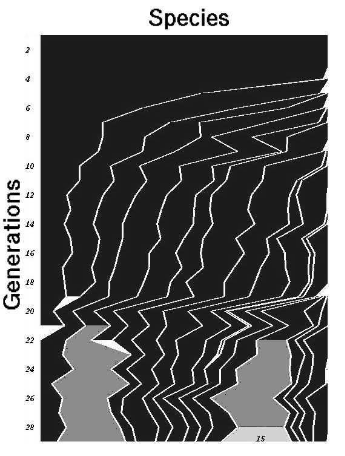
\includegraphics[width=0.50\textwidth]{Figures/chapter_ne/ne_neat_speciate_vis.png} % Include the figure image
	\caption{Visualizing NEAT's Speciation Mechanism while Solving the Double Pole Balancing Problem (\cite{stanley2002evolving})}
	\label{fig:neat_speciate_vis} % Unique label used for referencing the figure in-text
\end{figure}

\parbreak\noindent Additionally, NEAT offers significant advantage over traditional gradient-based methods, that is, it does not require the objective function or for the resulting neural network to be differentiable. While conventional training relies on backpropagation and gradient descent, NEAT evaluates candidate networks based soley on their performance. This makes it applicable to a wider range of problems, including those with discrete, noisy, or non-differentiable environments (\cite{stanley2002evolving}). As a result, NEAT provides greater flexibility in domains where gradient information is unreliable or simply unavailable.

\parbreak\noindent Despite its strengths, NEAT faces several challenges. One of the most significant is its computational costs. The simultaneous evolution of topology and weights requires high computation feature extraction (\cite{peng2018neat}). Additionally, because NEAT evolves arbitrary network topologies rather than layered architectures, it cannot leverage efficient matrix operations for forward propagation. Instead, each neuron must be activated individually following a topological sort, resulting in slower network evaluation. Another challenge is the sensitivity in fine-tuning the hyperparameters such as the mutation rates, speciation thresholds, and population size. Improper tuning can lead to issues such as stagnation, overfitting, or excessive computational overhead (\cite{stanley2002evolving}).

\parbreak\noindent Overall, NEAT's strengths far outweigh its limitations, particular in optimization problems requiring innovative architectures or dynamic adaptability. As computational resources improve, many of NEAT's challenges may become less significant, further establishing its role as a powerful tool in neuroevolution.

\subsection{HyperNEAT, a NEAT extension}
Hypercube-based Neuroevolution of Augmenting Topologies (HyperNEAT), an extension of NEAT was developed to address the challenges in problems with inherent geometric or spacial structures. While NEAT excels at evolving neural networks by optimizing both topology and weights, it does not necessarily exploit the spatial relationships present in real-world tasks such as image recognition (\cite{stanley2009hypercube}). HyperNEAT extends NEAT by introducing an indirect encoding mechanisms using Compositional Pattern Producing Networks (CPNNs), which represent neural network connectivity patterns as mathematical functions.

\parbreak\noindent CPPNs allow HyperNEAT to encode complex patterns of connectivity in a compact fashion. Instead of explicitly defining each connection, CPPNs describe how connections between neurons should be formed based on their geometric position. This approach is particularly advantageous for large-scale networks, where explicitly encoding all connection would be computationally prohibitive. HyperNEAT generates neural networks that are not only scalable but also better suited to exploit the inherent spatial structure of the task (\cite{stanley2009hypercube}).

\parbreak\noindent CPPNs can be thought of as a phenotype that is a pattern in space. Each coordinate in that space represents some level of expression as an output of a function that encodes the phenotype. The CPPN is a neural network that takes in coordinates and outputs a weight value which maps to a plane as shown in Figure \ref{fig:ne_hyperneat_cppn}. HyperNEAT revolves around three main steps, namely, substrate creation, CPPN evolution, and phenotype generation. The HyperNEAT algorithm is shown in Algorithm \ref{alg:hyperneat_algorithm}.

\parbreak\noindent \paragraph{Substrate Creation} involves the creation of a substrate which is a geometric representation of the neural network, where are nodes are arranged in such a way that reflects the spatial relationship inherent in the task (\cite{stanley2009hypercube}). For example, in robotic control tasks, the substrate might reflect the physical layout of sensors and actuators while in image recognition tasks the substrate might be a grid corresponding to pixel locations.

\parbreak\noindent \paragraph{CPPN Evolution} involve evolving CPPN networks using the NEAT algorithm. As mentioned, unlike a direct encoding where each connection is explicitly represented, the CPPN operates as a compact function that spits out weight values based on the relationship of underlying nodes in question. The CPPN's evolution is guided by a fitness function that evaluates the performance of the networks generated by the pattern encoded as a result from the CPPN (\cite{stanley2009hypercube}).

\parbreak\noindent \paragraph{Phenotype Generation} is the creation of the phenotype (the actual neural network) by querying the evolved CPPN for each pair of nodes in the substrate. For every set of nodes, the CPPN takes their spatial coordinates as inputs and returns a weight  representing the connections characteristics such as the weight values, whether they exist or not, etc. CPPN is essentially the blueprint that maps out the phenotype (\cite{stanley2009hypercube}). The resulting networks inherit the regularities encoded by the CPPN which allows them to better integrate unseen data based on their spatial relationship.

\parbreak
\begin{figure}[H] % Use [H] to suppress floating and place the figure/table exactly where it is specified in the text
	\centering % Horizontally center the figure on the page
	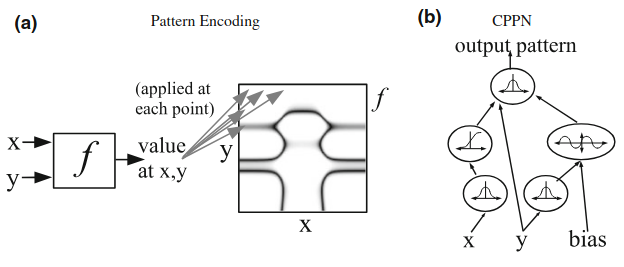
\includegraphics[width=\textwidth]{Figures/chapter_ne/ne_hyperneat_cppn.png} % Include the figure image
	\caption{CPPN encoding where \textbf{a} represents the pattern encoding as a result from output of the CPPN in \text{b} (\cite{d2014hyperneat})}
	\label{fig:ne_hyperneat_cppn} % Unique label used for referencing the figure in-text
\end{figure}

\begin{algorithm}[H]
	\caption{HyperNEAT algorithm (\cite{stanley2009hypercube})}\label{alg:hyperneat_algorithm}
	\begin{algorithmic}[1]
        \item Choose substrate configuration (i.e, node layout and input-output assignments)
        \item Initialize the poopulation of minimal CPPNs with random weights
        \item Repeat until a solution is found:
        \item \:\: For each member of the population
        \item \:\:\:\: Query its CPPN for the weight of each other connection in the substrate. If the absolute value of the output exceeds a threshold magnitude, create the connection with a weight scaled proportionally to the output value
        \item \:\:\:\: Run the substrate as an ANN in the task domain to ascertain fitness
        \item \:\: Reproduce the CPPNs according to the NEAT method to produce the next generation population
    \end{algorithmic}
\end{algorithm}

\parbreak\noindent One of HyperNEAT's notable strength resides in its ability to produce networks with inherent symmetries and patterns that mirror the problem domain (which is shown in Figure \ref{fig:ne_hyperneat_cppn}). This ability to capture and leverage geometric regularities makes HyperNEAT desirable in domains where spatial relationships are crucial. Although powerful, HyperNEAT can suffer from computational overhead, especially during the querying process of the CPPN to produce neural network solutions of a large scale (\cite{stanley2009hypercube}). Applications where HyperNEAT has been used include training agents to play games, learning autonomous agent controllers, robocup simulations, etc (\cite{kowaliw2014growing}).
%------------------------------------------------

%------------------------------------------------
\chapterimage{}
\chapterspaceabove{6.75cm}
\chapterspacebelow{7.25cm} 
\chapter{Gene Expression Programming}\label{chapter:gep}
This chapter explores the foundational principles of GEP, its integration with neural networks through gene expression programming neural networks, and current research, highlighting GEP's role as a transformative tool in computational intelligence. An introduction to GEP is given in Section \ref{sec:gep_introduction}, after which the historical background is discussed in Section \ref{sec:gep_historical_background}. Section \ref{sec:gep_core_concepts} provides the reader with the fundamental mechanics behind GEP and it's neural network extension, GEP-NN. The strengths and challenges of GEP are discussed in Section \ref{sec:gep_strenght_challenges} and finally, Section \ref{sec:gep_current_research} summarizes recent advancements made in GEP and GEP-NN.


\section{Introduction}\label{sec:gep_introduction}
Gene Expression Programming (GEP) is an evolutionary algorithm that blends the strengths of genetic programming and genetic algorithms seen in Chapter \ref{chapter_ea} in order to solve complex computational problems. Introduced by Candida Ferreira in 2001, GEP is distinguished by its unique encoding method which decouples the genotype (fixed-length chromosome) from the phenotype (expression trees) (\cite{ferreira2006gene}). This dual representation enables the efficiency and versatility that GEP brings, enabling it to explore complex solution spaces with a balance of exploration and exploitation.

\parbreak\noindent In GEP, candidate solution are represented as fixed length linear chromosomes composed of genes, which are later translated into function programs or expressions. This genotype-to-phenotype mapping is powered by Karva notation and allows GEP to maintain the structural integrity of solutions during  genetic operators like crossover and mutation, addressing the key limitation in genetic programming where such genetic operations often disrupt and result in non-functional expressions.

\parbreak\noindent GEP generally excels in tasks requiring symbolic regression, optimization, and automated problem-solving. It has been used in applications ranging from classification problems (CP) to automatic model design problems (AMDP) (\cite{zhong2017gene}). One of its most innovative applications is in the creation of neural networks using GEP-NN. Gene Expression Programming Neural Networks (GEP-NN) is an extension on GEP whereby the topology and weights of a neural network are evolved using the principles of GEP. The neural network is encoded in three separate domain, namely, the normal GEP genotype domain representing the nodes of the neural net, and two additional domains, \textit{Dw} and \textit{Dt} which encode the weight connection and threshold values respectively (\cite{ferreira2006gene}).

\section{Historical Development of GEP}\label{sec:gep_historical_background}
The origins of Gene Expression Programming (GEP) can be traced to Candida Ferreira's groundbreaking in the early 2000s (\cite{ferreira2006gene}). In attempt to overcome the limitations of genetic algorithms (GA) and genetic programming (GP), Ferreira introduced GEP in 2001 as a novel evolutionary approach that decoupled the representation of solutions in their genotype form from their phenotype functional expression representation. The introduction of this algorithm addressed challenges such as inefficiencies in genetic operations and the difficulty of evolving structurally complex solutions. This established GEP as a versatile tool for solving a wide range of optimization problems (\cite{ferreira2006gene}).

\parbreak\noindent Ferreira's development of GEP was motivated by limitations of GP, particularly the disruption of functional expressions during evolutionary genetic operators such as crossover and mutation. By encoding solutions as fixed-length linear chromosome, GEP ensured that when these genetic operations were applied, it would not compromise the integrity of functional structures. These chromosomes were then expressed in their phenotype form as parse trees or directed graphs, showcasing its genotype-phenotype mapping flexibility (\cite{ferreira2006gene}).

\parbreak\noindent The publication of Ferreira's book, \textit{Gene Expression Programming: Mathematical Modeling by an Artificial Intelligence}, in 2001 sparked interest in the broader research community. Early experiments demonstrated GEP's superiority in tasks such as symbolic regressions, where it outperformed competing optimization algorithms by producing simpler, more interpretable solutions.

\parbreak\noindent By the mid-2000s, GEP was integrated with neural networks to optimize topology and weights, giving rise to gene expression programming neural networks (GEP-NN). This marked a significant advancement, as GEP's ability to evolve the entire architecture established it as a powerful alternative to traditional training methods like backpropagation (\cite{ferreira2006gene}).

\parbreak\noindent Initially focused on symbolic regressions, GEP quickly found applications in other fields such as engineering and medicine (\cite{malik2016application}, \cite{kusy2013application}). Researchers began adapting GEP to solve multi-objective problems and handle dynamic environments, broadening its usage (\cite{zheng2012multi}). Today, GEP is recognized as a versatile and scalable evolutionary algorithm and has been seen to be used in many other fields such as the optimization of blasting patterns in mines (\cite{bayat2022blasting}), and its usage in predicting pavement performance, an essential metric used in the rehabilitation and reconstruction of roads (\cite{mazari2016prediction}).

\section{Core Concepts in Gene Expression Programming}\label{sec:gep_core_concepts}

\begin{figure}[H] % Use [H] to suppress floating and place the figure/table exactly where it is specified in the text
	\centering % Horizontally center the figure on the page
	\includesvg[width=\textwidth]{Figures/chapter_gep/gep_algorithm.svg} % Include the figure image
	\caption{Gene Expression Programming Algorithm (adapted from \cite{ferreira2006gene})}
	\label{fig:gep_algorithm} % Unique label used for referencing the figure in-text
\end{figure}

\parbreak Gene Expression Programming (GEP) is defined by its unique approach to encoding solutions, translating genetic representations into guaranteed functional outputs, and employing a suite of genetic operators to evolve populations over successive generations mimicking evolutionary processes. Understanding these core concepts is essential in grasping the algorithm that this paper proposes. The basic GEP algorithm can be summarised as shown in Figure \ref{fig:gep_algorithm}.

\subsection{The Genome}
\subsubsection{GEP}
Understanding how GEP works begins with understanding how the genome is constructed. The chromosome is a linear fixed-length string made up of symbols (genes). The chromosome represents the genotype, and can then be decoded to represent the expression tree which is the phenotype (\cite{ferreira2006gene}). For example, consider the following algebraic expression:
\begin{ceqn}
    \begin{equation}\label{alg:gep_chromsome_example}
        \sqrt{(a \times b) + c}
    \end{equation}
\end{ceqn}

\parbreak\noindent This equation can be represented as an expression tree seen in Figure \ref{alg:gep_chromsome_example}, representing the phenotype, where $Q$ represents the square root function.

\parbreak\noindent GEP makes use of \textit{Karva Notation} as a genotype-phenotype mapping scheme which maps an expression tree into a \textit{K-expression}. It works by simply reading the expression tree left-to-right and top-to-bottom. The expression tree seen in Figure \ref{alg:gep_chromsome_example} can then be represented in its genotype form (K-expression) as follows:
\begin{ceqn}
\begin{equation}
    \begin{array}{cccccc}
        0 & 1 & 2 & 3 & 4 & 5\\
        Q & + & \times & c & a & b
    \end{array}
\end{equation}
\end{ceqn}

\parbreak
\begin{figure}[H] % Use [H] to suppress floating and place the figure/table exactly where it is specified in the text
	\centering % Horizontally center the figure on the page
	\includesvg[width=0.3\textwidth]{Figures/chapter_gep/chapter_gep_phenotype.svg} % Include the figure image
	\caption{Example Expression Tree For Mathematical Equation \ref{alg:gep_chromsome_example}}
	\label{fig:gep_phenotype_example} % Unique label used for referencing the figure in-text
\end{figure}
  
\parbreak\noindent Although GEP primarily uses k-expressions as its mapping scheme, postfix and prefix configurations exist - using the expression tree in Figure \ref{fig:gep_phenotype_example}, postfix would be encoded as seen in Equation \ref{alg:postfix}, and prefix would be encoded as seen in Equation \ref{alg:prefix}.
\begin{ceqn}
    \begin{equation}\label{alg:postfix}
        \begin{array}{cccccc}
            0 & 1 & 2 & 3 & 4 & 5\\
            a & b & \times & c & + & Q
        \end{array}
    \end{equation}
\end{ceqn}

\begin{ceqn}
    \begin{equation}\label{alg:prefix}
        \begin{array}{cccccc}
            0 & 1 & 2 & 3 & 4 & 5\\
            Q & + & \times & a & b & c
        \end{array}
    \end{equation}
\end{ceqn}

\subsubsection{GEP-NN}
\noindent As mentioned, GEP extends its methodology to encode and evolve neural networks due to its simplicity and plasticity. The general neural network seen in Section \ref{sec:nn_nutshell} can be easily translated in an expression tree as shown in Figure \ref{fig:gep_nn_example} where \textit{a} and \textit{b} represents the inputs \textit{i1} and \textit{i2} respectively, and \textit{D} represents a function with connectivity two which serves as the weighted sum (\cite{ferreira2006gene}).

\begin{figure}[H] % Use [H] to suppress floating and place the figure/table exactly where it is specified in the text
	\centering % Horizontally center the figure on the page
	\includesvg[width=0.8\textwidth]{Figures/chapter_gep/chapter_gep_nn_example.svg} % Include the figure image
	\caption{Example Neural Network and its Expression Tree Counterpart}
	\label{fig:gep_nn_example} % Unique label used for referencing the figure in-text
\end{figure}

\subsection{Structural Organization of Genes}
\subsubsection{GEP}
GEP genes are composed of two different domains, namely, the head and the tail. The head domain is used to encode the function symbols used in the optimization problem while the tail serves as a buffer of terminal symbols in order to guarantee that functional expression trees are generated. The length of the genome is made up of the head and the tail. It should be noted that the head can contain both function symbols and terminal symbols. The length of the head is predefined, and the tail is calculated as follows (\cite{ferreira2006gene}):
\begin{ceqn}
    \begin{equation}\label{alg:prefix}
        t = h \times (n_{max} - 1) + 1
    \end{equation}
\end{ceqn}

\noindent where:
\begin{itemize}
    \item \textbf{$t$} is the length of the tail
    \item \textbf{$h$} is the length of the head (predefined)
    \item \textbf{$n_{max}$} is the number of arguments of the function with the most arguments (also called the maximum arity)
\end{itemize}

\parbreak\noindent As an example with reference to the expression to mathematical Equation \ref{alg:gep_chromsome_example}, the function set would be $F=\{Q,\times,+\}$ and the terminal set would be $T=\{a,b,c\}$. The maximum arity $n_{max}$ would be 2 as multiplication and addition both take in two arguments (as opposed to Q/square root which takes one argument). Provided a head size of 4 was chosen, the tail length would then be $t = 4 \times (2 - 1) + 1 = 5$. The chromosome length would as a result be $h + t = 4 + 5 = 9$. A chromosome representing Equation \ref{alg:gep_chromsome_example} could look as follows (tail is in bold):
\begin{ceqn}
    \begin{equation}\label{alg:gep_full_chromosome}
        \begin{array}{ccccccccc}
            0 & 1 & 2 & 3 & 4 & 5 & 6 & 7 & 8\\
            Q & + & \times & a & \textbf{b} & \textbf{c} & \textbf{a} & \textbf{b} & \textbf{a}
        \end{array}
    \end{equation}
\end{ceqn}

\parbreak\noindent The tail acts like a reservoir of terminal symbols meaning that functional expression trees are always a given. Not all terminal symbols are guaranteed to be used in the phenotype representation - those symbols that are not used are referred to as the non-coding region, whilst the symbols that are used is referred as the coding region (\cite{ferreira2006gene}).

\parbreak\noindent GEP chromosomes do not necessarily need to contain only one gene - multigenic systems can easily be represented, for example:
\begin{ceqn}
    \begin{equation}\label{alg:gep_full_chromosome}
        \begin{array}{cccccccccccccccccc}
            0 & 1 & 2 & 3 & 4 & 5 & 6 & 7 & 8 & 9 & 0 & 1 & 2 & 3 & 4 & 5 & 6 & 7 \\
            Q & + & \times & a & \textbf{b} & \textbf{c} & \textbf{a} & \textbf{b} & \textbf{a} & + & + & Q & b & \textbf{a} & \textbf{a} & \textbf{b} & \textbf{c} & \textbf{a}
        \end{array}
    \end{equation}
\end{ceqn}

\parbreak\noindent These two genes represent two respective sub-expression trees. By incorporating mutligenic systems, complex genomes can be created by smaller genomes, a common occurrence seen in nature (\cite{ferreira2006gene}). For optimization problems with multiple outputs such as classification problems, the different sub-expression trees are seen as autonomous agents working together to each produce a particular output for a set of given inputs (\cite{ferreira2006gene}). Sub-expression trees can also be combined using a linking function to form a larger expression tree as shown in Figure \ref{fig:gep_linking_function} (using Equation \ref{alg:gep_full_chromosome}). Multigenic chromosomes guide the evolution in modular structures, a small building block in order to create more complex structure.

\parbreak
\begin{figure}[H] % Use [H] to suppress floating and place the figure/table exactly where it is specified in the text
	\centering % Horizontally center the figure on the page
	\includesvg[width=\textwidth]{Figures/chapter_gep/chapter_gep_linking.svg} % Include the figure image
	\caption{Example of Linking Function to Connect Sub Expression Trees}
	\label{fig:gep_linking_function} % Unique label used for referencing the figure in-text
\end{figure}

\subsubsection{GEP-NN}
When using GEP genomes to represent neural networks, two additional domains are required in order to encode the weights of the connectivities between nodes, and the thresholds used when applying an activation function (\cite{ferreira2006gene}). These two domains, denoted, \textit{Dw} and \textit{Dt}, are encoded in their own regions within the chromosome. Depending on the problem at hand in which a neural network needs to be designed for, these additional domains are characterized by the outcome. In some instances, the threshold domain is not required, especially when using activation functions that are non-linear. The chromosome for the expression tree seen in Figure \ref{fig:gep_nn_example} would look as follows:
\begin{ceqn}
    \begin{equation}\label{alg:gep__nn_chromosome_example}
        \begin{array}{cccccccccccccccccc}
            0 & 1 & 2 & 3 & 4 & 5 & 6 & 7 & 8 & 9 & 0 & 1 & 2 \\
            D & D & D & a & b & a & b & \textbf{1} & \textbf{2} & \textbf{3} & \textbf{4} & \textbf{5} & \textbf{6} &
        \end{array}
    \end{equation}
\end{ceqn}

\noindent where position 0 to 6 represents the neural network gene region, and the positions in bold are the weights. Typically, the \textit{Dw} gene stores indices and is used to fetch indices from a lookup array as necessary. This array could look as \textit{$W = \{-1.2, 0.8, -0.3, 1.4, 0.5, -2.0\}$}. The length of the \textit{Dw} domain is calculated using \textit{$Dw_{length} = h \times n_{max}$} and the length of \textit{Dt} is calculated using \textit{$Dt_{length} = h$} (\cite{ferreira2006gene}).


\subsection{Genotype Operators}\label{sec:gep_genetic_operators}
GEP employs a variety of genetic operators to balance exploration and exploitation. These operators are tailored to its fixed-length genotype and ensure syntactically correct phenotypes. These genetic operators are modified in various ways to extend its application in the GEP-NN domain.

\subsubsection{Mutation}
Mutation in GEP is one of the most efficient genetic operators allowing candidate solutions to adapt very quickly. For a given mutation $p_m$, two one-mutations operations are applied to the chromosome. If the mutation point happens to be in the head, the mutation can result in symbols from both the function and terminal set whereas if it occurs in the tail, only symbols from the terminal set can be chosen (\cite{ferreira2006gene}). More importantly, a single mutation can have a profound effect on the phenotype, especially if the mutation involves change from function set symbols to terminal set symbols as the entire expression tree structure would be altered. In the GEP-NN counterpart, mutation is able to also occur in the \textit{Dw} and \textit{Dt} domains using novel schemes for mutating constants (\cite{ferreira2006gene}).

\subsubsection{Inversion}
GEP Inversion is similar to the inversion scheme seen in Section \ref{sec:ea_mutation} with the difference that it operates within the head of the chromosome which ensures that no matter what start and termination points are chosen, syntactically correct programs will always be produced (\cite{ferreira2006gene}). In GEP-NN, inversion is applicable to both the \textit{Dw} and \textit{Dt} and works as implied for a given inversion rate, \textit{$p_i$}. Inversion in this domain ensures the circulation of weights and thresholds within the genetic pool.

\subsubsection{Transposition}
Transposition moves a segment of a gene to another location within the same chromosome in an attempt to create repetitive sequences within the phenotype. There are three kinds of transposable elements in GEP (\cite{ferreira2006gene}):

\begin{enumerate}
    \item \textbf{Insertion Sequence (IS) Elements} - Fragments beginning with either a function or terminal that transpose to the head of genes, except the root.
    \item \textbf{Root Insertion Sequence (RIS) Elements} - Fragments beginning with only a function that transpose to the root genes.
    \item \textbf{Entire genes} that transpose to the beginning of chromosomes.
\end{enumerate}

\parbreak\noindent During the transposition of IS elements of transposition rate, \textit{$p_{is}$}, any sequence within the element can become an IS element. This element is then copied at the place of origin and inserted at the randomly chosen point in the gene head (except the start position) (\cite{ferreira2006gene}). Its worth noting that once the IS element is copied, it can only be inserted strictly within the gene head to ensure functional expressions.

\parbreak\noindent During the transposition of RIS elements of transposition rate, \textit{$p_{ris}$}, a sequence beginning with a function is chosen, and inserted in a randomly chosen start and end position. RIS differs from IS transposition in its ability to have the root of the chromosome as the start point (\Cite{ferreira2006gene}).

\parbreak\noindent During gene transposition of transposition rate, \textit{$p_{gr}$}, entire genes inside the chromosome are transposed and in effect make repeatable structures amongst chromosomes that consist of more than one expression tree (\cite{ferreira2006gene}).

\parbreak\noindent Transposition can also be applied to GEP-NN genes in the \textit{Dw} and \textit{Dt} domain, with the added advantage that any sequence in the domain can be chosen as the transposition element (\cite{ferreira2006gene}). This ensures that new weight and thresholds get tested at different connectivity locations within the neural network.

\subsubsection{One-point Recombination}
One-point recombination involves two randomly chosen parents to be paired side by side and split up, producing two offspring. Its recombination rate is specified as \textit{$p_{1r}$}. It works exactly as what was seen with single point crossover in Section \ref{sec:ea_mutation} (\cite{ferreira2006gene}). One-point recombination can have monstrous effects disrupting old building blocks and continually forming new ones.

\subsubsection{Two-point Recombination}
Two-point recombination involves two randomly chosen parents to be paired side by side and split at two points randomly, producing two offspring. Its recombination rate is specified as \textit{$p_{2r}$}. Two-point recombination is far more disruptive than one-point recombination since genetic material is combined more thoroughly thereby destroying existing building blocks and creating new ones. When dealing with GEP-NN chromosomes that consist of multiple sub-NNs, two-point recombination is restricted within the sub-NN in order to allow fine grain control and ensure that weights and thresholds amongst other sub-NNs are kept intact (\cite{ferreira2006gene}).

\subsubsection{Gene Recombination}
Gene recombination operates in the same fashion as gene transposition, that is, entire genes are exchanges between two parent chromosomes, at a gene recombination rate, \textit{$p_{gr}$}. The intent of gene recombination is not to create genes, but instead test different configuration of existing genes, especially in scenarios where they are collectively put together through a linking function (\cite{ferreira2006gene}). Likewise, in GEP-NN chromosomes, gene recombination serves as mechanism to exchange entire sub-NNs as a balance mechanism between exploration and exploitation.

\subsection{Population and Fitness}
As in any evolutionary algorithm, the initial population of candidate solutions are generated through a randomized approach. In the case of GEP, these chromosomes are generated in a way that is adhered to the head and tail constraints mentioned, that is, the head would consist of symbols drawn from the function and terminal set whereas the tail would consist of symbols drawn only from the terminal set (\cite{ferreira2006gene}). After the population is initialized, a fitness function is applied to each individual. According to Ferreira, for populations of a small size or set of fitness cases not broad enough, the population in its entirety might produce a fitness of 0. To mitigate this issue, GEP employs that a start-up control mechanism is used to in which an initial population is generated until a single viable solution is obtained. In doing so, GEP evolves candidate solutions that are descendants of a sole viable founder.

\parbreak\noindent Fitness evaluations measure how well an individual solves the given problem, guiding the selection of individuals for reproduction. GEP proposes a few fitness functions that can be used depending on the task at hand. A few fitness functions will be discussed that are applicable to different optimization problems.

\subsubsection{Fitness Functions for Symbolic Regression}
Symbolic regression tasks involves finding a symbolic expression that excels at numeric prediction. There are four main fitness functions that Ferreira discusses which are summarised as follows:

\begin{enumerate}
    \item \textbf{Number of Hits} Fitness Function - This fitness functions is designed for models that need to perform well for numerous fitness cases within a certain error, whether it is absolute or relative (\cite{ferreira2006gene}). The fitness of an individual candidate solution \textit{i} for fitness case \textit{j} is evaluated by the formula:
    \begin{ceqn}
        \begin{equation}\label{alg:number_of_hits}
            f_{ij} =
            \begin{cases} 
                1 \:\: if \:\: E_{ij}  <= p\\
                0 \:\: otherwise
            \end{cases}
        \end{equation}
    \end{ceqn}

    \noindent where \textit{p} is the precision and \textit{$E_{ij}$} is the error of candidate solution $i$ and fitness case $j$ (\cite{ferreira2006gene}). Depending on whether the error is relative or absolute is defined by the following equations respectively:

    \begin{ceqn}
        \begin{equation}\label{alg:relative_error}
            E_{ij} = |P_{ij} - T_{ij}|
        \end{equation}
    \end{ceqn}

    \begin{ceqn}
        \begin{equation}\label{alg:absolute_error}
            E_{ij} = |\frac{P_{ij} - T_{ij}}{T_j} \times 100|
        \end{equation}
    \end{ceqn}

    \noindent where \textit{$P_{ij}$} is the predicted value for candidate solution \textit{i} and fitness case \textit{j}, and \textit{$T_j$} is the target value for fitness case \textit{j}.

    \item \textbf{Precision and Selection Range} Fitness Function - This fitness function operates by means of a selection range whereby if the candidate solutions fitness performs well it contributes to the overall fitness and if it does poorly it weakens the overall fitness (\cite{ferreira2006gene}). The fitness can use either relative error or absolute error as follows:
    \begin{ceqn}
        \begin{equation}\label{alg:relative_error2}
            f_i = \sum_{j=1}^{n}(R-E_{ij})
        \end{equation}
    \end{ceqn}

    \noindent where $E_{ij}$ refers to Equation \ref{alg:relative_error} if using relative error, and $E_{ij}$ refers to Equation \ref{alg:absolute_error} is using absolute error.

    \item \textbf{Mean Squared Error} Fitness Function - This fitness function is one of the most widely used and is based on the standard mean squared error, \textit{$E_i$} (\cite{ferreira2006gene}). The mean squared error is calculated as follows:
    \begin{ceqn}
        \begin{equation}\label{alg:mean_square_error}
            E_i = \frac{1}{n}\sum_{j=1}^{n}(E_{ij})^2
        \end{equation}
    \end{ceqn}

    \noindent where $E_{ij}$ refers to Equation \ref{alg:relative_error} if using relative error, and $E_{ij}$ refers to Equation \ref{alg:absolute_error} is using absolute error. In order for a perfect fitness to occur, \textit{$P_{ij}$} needs to equal \textit{$T_j$} for all fitness cases meaning that the mean squared error ranges from 0 to infinity. Its worth noting that this fitness function can't be used for evolutionary selection mechanisms that involve proportionate selection as the fitness in this scheme needs to increase. In such as situation, the following fitness evaluation needs to be used ranging its fitness number from 0 to 1000:
    \begin{ceqn}
        \begin{equation}\label{alg:mean_square_error_fitness}
            f_i = 1000 \times \frac{1}{1 + E_i}
        \end{equation}
    \end{ceqn}

    \item \textbf{R-square} Fitness Function - This fitness function is based on the standard R-square returning the square of the Pearson product moment correlation coefficient, \textit{$R_i$}, and is calculated as follows (\cite{ferreira2006gene}):
    \begin{ceqn}
        \begin{equation}\label{alg:r_square}
            R_i = \frac{n\sum_{j=1}^{n}(T_jP_{ij}) - (\sum_{j=1}^{n}T_j)(\sum_{j=1}^{n}P_{ij})}{\sqrt{[n\sum_{j=1}^{n}T_j^2 - (\sum_{j=1}^{n}T_j)^2][n\sum_{j=1}^{n}P_{ij}^2 - (\sum_{j=1}^{n}P_{ij})^2]}}
        \end{equation}
    \end{ceqn}

    \noindent When $R=1$, there is an optimal positive linear correlation, when $R=-1$, an optimal negative linear correlation between \textit{P} and \textit{T}, and when $R=0$, there is no correlation. The fitness is then calculated using the equation below, meaning that the fitness ranges from 0 to 1000.
    \begin{ceqn}
        \begin{equation}\label{alg:r_square}
            f_i = 1000 \times R_i^2
        \end{equation}
    \end{ceqn}
\end{enumerate}

\subsubsection{Fitness Functions for Classification and Logic Synthesis}
Classification optimization problems focus on finding a model that accurately maps inputs to predefined categories or classes whereas logic synthesis focuses on optimizing logic circuits to implement Boolean functions efficiently. GEP has applications in both with a wide selection of fitness functions that Ferreira mentions:

\begin{enumerate}
    \item \textbf{Number of Hits} Fitness Function - This fitness function corresponds to the number of samples correctly classified. The fitness of an individual candidate solution, \textit{i}, can be evaluated as follows (\cite{ferreira2006gene}):
    \begin{ceqn}
        \begin{equation}\label{alg:class_number_of_hits}
            f_i = h
        \end{equation}
    \end{ceqn}

    \noindent where \textit{h} is the number of fitness cases evaluated correctly.

    \item \textbf{Hits with Penalty} Fitness Function - This fitness function mitigates the chances of favoring candidate solutions that end up in a local optima. It works by recording the number of true positives (\textit{$TP_i$}) and true negatives (\textit{$TN_i$}). The fitness function is then calculated as follows (\cite{ferreira2006gene}):
    \begin{ceqn}
        \begin{equation}\label{alg:class_hits_with_penalty}
            f_{i} =
            \begin{cases} 
                0 \:\: if \:\: TP_i=0\:\:OR\:\:TN_i=0 \\
                h \:\: otherwise
            \end{cases}
        \end{equation}
    \end{ceqn}

    \noindent where \textit{h} is the number of fitness cases evaluated correctly, that is $h = TP_i + TN_i$. The fitness, \textit{$f_i$} has a maximum value as per Equation \ref{alg:class_number_of_hits}.

    \item \textbf{Sensitivity/Specificity} Fitness Function - This fitness function is based on sensitivity and specificity indicators. The sensitivity indicator reflects the probability that a fitness case detects a true positive in proportion to a positive fitness case. The specificity indicator reflects the probability that a fitness case detects a true negative in proportion to a negative fitness cases (\cite{ferreira2006gene}). These two indicators are calculated as follows:
    \begin{ceqn}
        \begin{equation}\label{alg:sensitivity}
            SE_i = \frac{TP_i}{TP_i + FN_i}
        \end{equation}
    \end{ceqn}

    \begin{ceqn}
        \begin{equation}\label{alg:specificity}
            SP_i = \frac{TN_i}{TN_i + FP_i}
        \end{equation}
    \end{ceqn}

    \noindent This sort of fitness function is useful in applications that involve highly unbalanced training sets since the result of multiplying both these indicators results in an index forcing the discovery of models that have both a high sensitivity and specificity probability (\cite{ferreira2006gene}). The fitness of candidate solution, \textit{i}, would be calculated as follows:
    \begin{ceqn}
        \begin{equation}\label{alg:ss_fitness}
            f_i = 1000 \times SS_i
        \end{equation}
    \end{ceqn}

    \noindent where $SS_i = SE_i \times SP_i$.

    \item \textbf{Positive Predictive Value / Negative Predictive Value} Fitness Function - This fitness function is based on the positive predictive value (PPV) and negative predictive value (NPV) indicators (\cite{ferreira2006gene}). PPV reflects the percentage of true positive cases and NPV reflects the percentage of false negatives cases. These two indicator are calculated as follows for candidate solution, \textit{i}:
    \begin{ceqn}
        \begin{equation}\label{alg:ppv}
            PPV_i = \frac{TP_i}{TP_i + FP_i}\:\:where \:\: TP_i + FP_i \neq 0
        \end{equation}
    \end{ceqn}

    \begin{ceqn}
        \begin{equation}\label{alg:npv}
            NPV_i = \frac{TN_i}{TN_i + FN_i}\:\:where \:\: TN_i + FN_i \neq 0
        \end{equation}
    \end{ceqn}
    \noindent Multiplying both these indicators results in the following equation:

    \begin{ceqn}
        \begin{equation}\label{alg:ppv_npv}
            PN_i = PPV_i \times NPV_i
        \end{equation}
    \end{ceqn}
    \noindent Evaluating the fitness of candidate solution, \textit{i}, is done as follows:
    \begin{ceqn}
        \begin{equation}\label{alg:ppv_fitness}
            f_i = 1000 \times PN_i
        \end{equation}
    \end{ceqn}

    \noindent Again, this fitness function ranges from 0 to 1000 with 1000 being the best solution.
\end{enumerate}

\subsection{Selection Mechanisms}
There are many selection mechanisms that can be used in evolutionary computing, a few of which have been discussed in Section \ref{sec:selection_mechanisms}. The selection operator chooses which candidate solutions are to be reproduced according to its fitness. GEP is not restricted to any specific selection mechanisms, however, in many of the optimization tasks that GEP was applied to in the original paper, elitism was used which produced favourable results (\cite{ferreira2006gene}).

\section{Strengths and Challenges}\label{sec:gep_strenght_challenges}
Gene Expression Programming is a powerful evolutionary algorithm that excels in solving complex problems through adaptive modeling and optimization. One of its greatest strengths lies in its genome representation of solutions. Unlike traditional Genetic Algorithms (GAs) and Genetic Programming (GP) (seen in Section \ref{sec:genetic_algorithms} and \ref{sec:genetic_programming} respectively), GEP decouples the genotype and phenotype, enabling better exploration capabilities in the solution space.  These separations allow for the evolution of highly complex expression while maintaining simplicity in genetic operations. GEP effectively mitigates one of the major challenges that GP struggles with which is enforcing complex rules in order to ensure that the evolved program is syntactically functional. During evolutionary processes of GP, special care needs to be taken in the way in which candidate solutions produce offspring, mutated, etc., all of which require often complex computation. By representing solutions as linear chromosomes that are later expressed as expression trees, GEP combines the advantages of linear and tree-based models, facilitating the discovery of sophisticated solutions without the complications of direct tree manipulations seen in GP. This structure enables the algorithm to evolve solutions that are both powerful and adaptable.

\parbreak\noindent GEP also presents certain challenges. One of the primary limitations is the computational cost associated with evolving large populations over many generations, especially when dealing with high-dimensional data or complex spaces (\cite{zhong2017gene}). As the complexity of the problem increases, so does the demand for computational resources, potentially making GEP less practical for time-sensitive tasks. As the case with many evolutionary algorithms, GEP may struggle with premature convergence, where population loses diversity and becomes trapped in a local optima, preventing the discovery of better candidate solutions. Maintaining genetic diversity within the population is critical but difficult, requiring well-balanced genetic operators to avoid stagnation. Parameter tuning such as selecting population size, mutation rates, function sets, etc., can be complex and problem-dependent, often times requiring trial and error to optimize performance. Many GEP adaptions make use of self adaption in an attempt to mitigate this problem, however, not much research has been done in this domain (\cite{zhong2017gene}). Balancing exploration and exploitation in the evolutionary search process remains a delicate task, often influencing the efficiency and success of GEP applications. Addressing these challenges requires a thoughtful algorithm design and problem specific customization to fully leverage GEP's flexibility and power.

\section{Current Research}\label{sec:gep_current_research}
As expressed in a comprehensive review article by \cite{zhong2017gene}, there have been numerous advancements in the research of GEP. These advancements can be categorized in three different areas of research in the context of this literature review:

\parbreak\noindent \paragraph{Adaption Design in GEP} is a mechanism that evolves control parameters such as population size, chromosome length, mutation rate, etc. within the evolutionary algorithm in order to improve optimization performance. There have been two adaptive GEP approaches, namely, AdaGEP and Adapative GEP. \textbf{AdaGEP} is a proposed extension of the original GEP algorithm that dynamically adjusts the number of active genes in chromosomes using a binary \textit{genemap} (\cite{bautu2007adagep}). Genes marked with a zero within this chromosome indicate that the subtree is ignored when being decoded while the being marked with one means that the subtree is active. This \textit{genemap} is evolved with the traditional GA genetic operators. The optimum number of genes used to solve the problem is evolved on the fly aiding to its increased performance over traditional GEP. \textbf{Adaptive GEP} makes use of feedback heuristic to modify operator execution probabilities (\cite{mwaura2009adaptive}). In other words, candidate solutions with higher fitness have increased probability of mutating and generating offspring as solutions with lower fitness are less likely to mutate and produce offspring.

\parbreak\noindent \paragraph{Cooperative Coevolutionary (CC)} is a framework aimed at solving large-scale optimization problems by breaking them into simpler subproblems. Each subproblem is then solved independently by making use of separate evolutionary algorithms with distinct subpopulations (\cite{zhong2017gene}). CC creates two problems to overcome - figuring out an effective way to decompose the problem, and finding a way to evaluate candidate solutions effectively. Sosa-Ascencio et al. proposed a new algorithm, CC-GEP, which encorporates GEP evolving two subpopulations, one representing the main program, and the other evolving automatically defined functions (ADFs) (\cite{zhong2017gene}). Furuholment et al. applied the concept of CC-GEP to the distributor's pallet packing problem which is an optimization problem to maximize the volume a set of distinct boxes certain dimensions on pallets, and the 3D process plant problem, both of which incorporated fitness sharing amongst the subpopulations to leverage a fine balance of exploration and exploitation of the search space.

\parbreak\noindent \paragraph{Parallel Design in GEP} is an approach to circumvent the issue of slow iterative evolution processes for large-scale and complex optimization problems. There are two parallelization models that researchers have applied GEP - the master-slave model and the island model (\cite{zhong2017gene}). The master-slave model operates by incorporating a master thread that manages the main program, while multiple slave threads handle subtasks concurrently. pGEP, an example of parallelization use in GEP, works my utilizing a master thread to manage GEP, with GPUs performing parallel fitness evaluations on the candidate solutions (\cite{zhong2017gene}). The island model, similar to the idea of CC, divides the population into subpopulations and each evolve independently by different processors. Subpopulations make use of fitness sharing amongst individuals to better enhance exploration and exploitation. Parallel niche gene expression programming (PNGEP) introduced by \cite{li2005prefix}, uses niching techniques to maintain  diversity, exchanging the best individuals through a shared pool amongst subpopulations (\cite{zhong2017gene}). Other models of parallelism include multiagent models whereby autonomous agents are used for task distribution.

\parbreak\noindent Other advancements presented in this survey included constant creation design mechanisms to better provide highly accurate constant values, GEPs application in automatic model design problems (AMDPs), and other problem specific optimization problems (\cite{zhong2017gene}). Another interesting, although not fully explored improvement in GEP is a study conducted by \cite{li2005prefix}, whereby the encoding scheme was investigated, forming a new algorithm coined prefix gene expression programming (P-GEP). As opposed to making use of the bread-width like encoding scheme used when converting from expression trees to karva notation, prefix notation is used, an example of which was seen in Equation \ref{alg:prefix}. Prefix notation has two major characteristics (\cite{li2005prefix}):

\begin{itemize}
    \item \textbf{Substructure Preserving characteristics}: Due to the nature in which prefix notation constructs the genome string, there is a more direct correlation between the genotype and phenotype. Nodes from the same sub-tree appear adjacent to one another meaning that subroutines can be better recognized as segments within the chromosomes thereby accounting for tighter genetic linkages. Having tightly linked genes positioned adjacent to one another means that the typical destructive genetic operators have less of monstrous effect thereby preserving structure and incorporating small change instead (\cite{li2005prefix}).
    \item \textbf{Inherent Hierarchy in Forming the Solution}: Because nodes from the same sub-tree appear adjacent to one another means that the hierarchies seen in the linear representation form incrementally and built upon the lower ones naturally (\cite{li2005prefix}). Figure \ref{fig:p_gep} illustrates this inherent hierarchy, and as well, shows that the genotype and phenotype both encode functional complexity similarly. Put simply, the linear chromosome representation and the expression tree both share the same level of expressiveness.
\end{itemize}

\parbreak\noindent Based on the experimental results of P-GEP, there are considerable improvements compared to the original GEP algorithm. By making use of prefix notation, the traditional GEP genetic operators are more protective for substructures which aids more refined search capabilities. GEP has two major shortcomings:

\begin{itemize}
    \item Constructing expression trees require frequent heap operations effecting the efficiency of the program. The larger the expression tree, the larger the number of heap operations.
    \item Expression trees are non-linear meaning that the larger the tree, meaning that non-linear memory address allocations become vastly complex
\end{itemize}

\parbreak
\begin{figure}[H] % Use [H] to suppress floating and place the figure/table exactly where it is specified in the text
        \centering % Horizontally center the figure on the page
        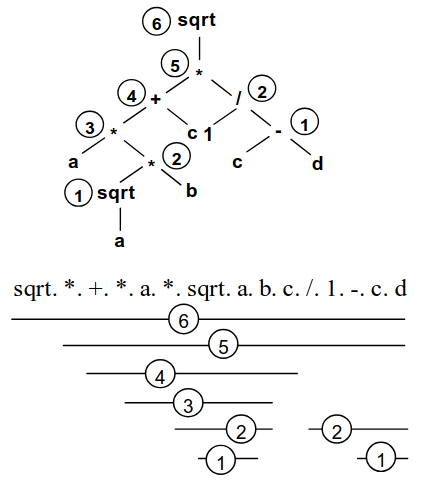
\includegraphics[width=0.5\textwidth]{Figures/chapter_gep/p_gep.png} % Include the figure image
        \caption{Illustration of hierarchy of P-GEP (\cite{li2005prefix})}
        \label{fig:p_gep} % Unique label used for referencing the figure in-text
\end{figure}

\noindent \textit{S\_GEP}, an extension of \textit{P-GEP}, has a unique characteristic to overcome the above shortcomings, which is its ability to evaluate the linear chromosomes using a stack (\cite{peng2014improved}). In order to evaluate the chromosome using a stack, the effective length of the gene needs to be calculated which represents the coding region. The effective gene length, \textit{el}, is calculated as shown in Algorithm \ref{alg:effective_length}.

\parbreak\noindent The effective gene length can then be used to evaluate the chromosome using a stack which is then visualized in Figure \ref{fig:gep_stack}. The effective gene is read in Polish notation fashion whereby the symbols are read right to left. As terminals are read, they are pushed onto the stack, and when a function symbol is encountered, it takes the terminals on the stack as input. The result is then pushed back on the stack and the process repeated until a single result remains. This mechanism can be summarized using Algorithm \ref{alg:gep_stack}.

\parbreak
\begin{algorithm}
	\caption{Effective gene length (adapted from \cite{peng2014improved})}\label{alg:effective_length}
	\begin{algorithmic}[1]
	% \Ensure $y = x^n$
	\item \textbf{Input}: String of gene symbols
	\item \textbf{Output}: eL
	\item Initialize variables $Len=1$ and $count=0$
	\item \textbf{while} scanning gene symbols starting from left to right
	\item \quad $Len = Len + 1$;
	\item \quad \textbf{if} current gene symbol is function:
	\item \quad \quad $count = count - 1$
	\item \quad \textbf{else}:
	\item \quad \quad $count = count - 1$
	\item \quad \textbf{if} $count < 0$
	\item \quad \quad return $eL=Len$ as output
\end{algorithmic}
\end{algorithm}

\parbreak
\begin{figure}[H] % Use [H] to suppress floating and place the figure/table exactly where it is specified in the text
    \centering % Horizontally center the figure on the page
    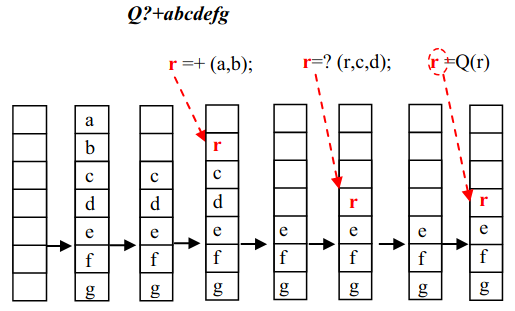
\includegraphics[width=0.75\textwidth]{Figures/chapter_gep/gep_stack.png} % Include the figure image
    \caption{Evaluation of GEP chromosome using stack (\cite{peng2014improved})}
    \label{fig:gep_stack} % Unique label used for referencing the figure in-text
\end{figure}

\parbreak\noindent \textit{S\_GEP} proved to show favourable results by outperforming traditional GEP in terms of its computation efficiency (\cite{peng2014improved}). Although applied primarily to regression problems, \textit{S\_GEP} poses as a powerful technique in general application, however, in the context of this research, GEP-NN specifically.

\parbreak
\begin{algorithm}
	\caption{S\_GEP Algorithm (adapted from \cite{peng2014improved})}\label{alg:gep_stack}
	\begin{algorithmic}[1]
	\item Calculate eL using Algorithm \ref{alg:effective_length}
	\item \textbf{while} reading effective gene from right to left using eL
	\item \quad \textbf{if} current gene is a terminal symbol:
	\item \quad \quad push terminal symbol on stack
	\item \quad \textbf{else if} current gene is function symbol:
	\item \quad \quad pull terminal symbols from stack and feed to function symbol
	\item \quad \quad push result value to stack
	\item pull value from stack and return
\end{algorithmic}
\end{algorithm}
%------------------------------------------------

%------------------------------------------------
\chapterimage{}
\chapterspaceabove{6.75cm}
\chapterspacebelow{7.25cm} 
\chapter{GEP-NEAT}\label{chapter:gep_neat}
This chapter covers GEP-NEAT, a blend between NEAT (covered in Chapter \ref{sec:ne_neat}) and gene expression programming (covered in Chapter \ref{chapter:gep}). An introduction to GEP-NEAT is given in Section \ref{sec:gep_neat_introduction}. The proposed algorithm is explained in-depth in Section \ref{sec:gep_neat_proposed_algorithm}, after which the prototype implementation is discussed in Section \ref{sec:gep_neat_protoype_implementation}. Finally, the prototype is applied to a few problems to benchmark the algorithm's performance in Section \ref{sec:gep_neat_model_validation}.

\section{Introduction}\label{sec:gep_neat_introduction}
As discussed in Chapter \ref{chapter:neuroevolution}, neuroevolution explores innovative strategies for optimising artificial neural networks (ANNs) using evolutionary algorithms (see Chapter \ref{chapter_ea}). Unlike conventional training methods such as backpropagation and gradient descent, which rely on differentiable loss functions and gradient-based updates, neuroevolution leverages Darwinian principles to evolve the topology of the neural network along with its weights and biases. This allows for the discovery of novel topologies, activation functions, and hyperparameters that may not be easily accessible through traditional approaches.

\parbreak\noindent A prominent example of this is the NEAT algorithm (Chapter \ref{sec:ne_neat}), which evolves both the structure and weights of neural weights simultaneously. NEAT's speciation mechanism preserves diversity and protects innovative structures during evolution, but one of its main challenges lies in its computational cost, largely due to the need for topological sorting during network evaluation, which makes the genotype-phenotype mapping and forward propagation computationally expensive. Nevertheless, NEAT's ability to operate without requiring differentiable functions makes it particularly well-suited for environments where gradient information is unaccessable.

\parbreak\noindent Building on these ideas, Gene Expression Programming (GEP) and its extension GEP-NN offer alternative evolutionary approaches that combine the global search capabilities of genetic algorithms with the expressive, tree-based representations of genetic programming. GEP introduces a novel genotype-to-phenotype mapping using Karva notation, enabling the evolution of complex, non-linear structures such as expression trees.

\parbreak\noindent The proposed algorithm, GEP-NEAT, integrates the representational power of GEP with the structural evolution principles of NEAT. It introduces several enhancements, including a reworked system for tracking innovation numbers, inspired by Richard Dawkins' concept of the meme. This mechanism enables more effective selection and mutation by identifying and preserving useful substructures across generations. Furthermore, GEP-NEAT addresses a key limitation in earlier GEP-based models by introducing a method for embedding bias information directly into the chromosome, thereby improving the expressiveness and learning capacity of evolved networks.

\section{Proposed Algorithm}\label{sec:gep_neat_proposed_algorithm}
\subsection{Evolutionary Life Cycle}
The goal of GEP-NEAT is to integrate the expressive representational capabilities of Karva notation from GEP with the neuroevolutionary mechanisms of NEAT, particularly its speciation and innovation tracking strategies. This hybrid approach aims to evolve neural network populations more effectively by combining the strengths of both paradigms.

\parbreak
\begin{figure}[H] % Use [H] to suppress floating and place the figure/table exactly where it is specified in the text
	\centering % Horizontally center the figure on the page
	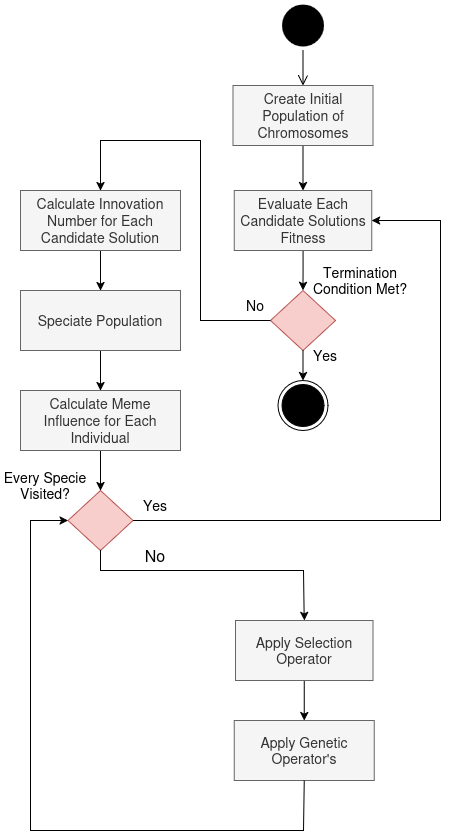
\includegraphics[width=0.65\textwidth]{Figures/chapter_gep_neat/gep_neat_framework.png} % Include the figure image
	\caption{Evolutionary Lifecycle of GEP-NEAT}
	\label{fig:gep_neat_framework} % Unique label used for referencing the figure in-text
\end{figure}

\parbreak\noindent At a high level, both NEAT and GEP follow a similar evolutionary cycle, that is, intialising a population, representing chromosomes, evaluating fitness, applying genetic operators, and iterating until a termination condition is met. The two approaches however diverge significantly in their internal mechanisms and innovations. NEAT introduces a sophisticated speciation mechanism, where historical gene information is tracked using innovation numbers. These are stored in a lookup table and used to calculate compatibility distance between individuals, allowing the population to be divided into species that evolve in parallel within their own niches (\cite{stanley2002evolving}).

\parbreak\noindent In contrast, GEP adheres more closely to the traditional genetic algorithm framework but distinguishes itself through a rich set of genetic operators that promote diversity and facilitate the emergence of reusable substructures, or building blocks, within chromosomes (\cite{ferreira2006gene}). Its use of Karva notation ensures syntactically valid expressions, making it particularly well-suited for evolving complex, non-linear representations.

\parbreak\noindent GEP-NEAT draws inspiration from both of these methodologies to form a unified framework, as illustrated in Figure \ref{fig:gep_neat_framework}. It leverages NEAT's innovation tracking and speciation to maintain diversity and protect novel structures, while adopting GEP's flexible chromosome representation to enable the evolution of expressive and structurally diverse neural networks.

\subsection{Representation}\label{sec:gep_neat_representation}
NEAT-GEP draws inspiration from the genotype-to-phenotype mapping introduced in Gene Expression Programming (GEP), particularly through the use of Karva notation, however, several modifications have been made to enhance the representation, starting with the adoption of prefix tree-style encoding. In traditional GEP, k-expressions are converted into expression trees by reading the linear string from left to right and top to bottom. While this method ensures syntactic correctness, it can become computationally expensive, especially when evaluating large populations or complex expressions since the expression tree must first be constructed from the expression string during each fitness evaluation. 

\parbreak\noindent As discussed in Chapter \ref{chapter:gep}, alternative encoding schemes such as prefix and postfix notation have been explored to address this limitation. On such approach, P-GEP, encodes linear chromosomes in prefix form. This representation improves the preservation of meaningful substructures during operations like crossover and mutation, which in turn supports more efficient and targeted exploration of the search space.

\parbreak\noindent Figure \ref{fig:gep_neat_p_gep} illustrates the differences between standard Karva notation and prefix notation, highlighting how subtrees - shown in purple, blue, and green - are affected by genetic operations. In standard Karva notation, these substructures are often disrupted during crossover, whereas prefix notation allows them to be preserved. For example, when a single-point crossover is applied between gene 3 and 4, the prefix-encoded chromosome maintains the integrity of its subtrees, whereas the same operation on a Karva-encoded chromosome may fragment them.

\parbreak
\begin{figure}[H] % Use [H] to suppress floating and place the figure/table exactly where it is specified in the text
	\centering % Horizontally center the figure on the page
	\includesvg[width=0.80\textwidth]{Figures/chapter_gep_neat/gep_neat_p_gep.svg} % Include the figure image
	\caption{GEP Encoding Scheme versus P-GEP Encoding Scheme}
	\label{fig:gep_neat_p_gep} % Unique label used for referencing the figure in-text
\end{figure}

\parbreak\noindent To illustrate how a GEP-NEAT chromosome is structured and functions, this chapter introduces a Simplified example. Consider a linear chromosome with a head size of $h = 3$ and a maximum function arity of $3$. Let the function set be ${D, T}$, where function $D$ takes two inputs and $T$ takes three, and the terminal set be ${a, b, c}$. According to GEP's formulation, the tail size is calculated using the formula:
\begin{ceqn}
	\begin{equation}
		t = h \times (n_{max} - 1) + 1 = 3 \times (3 - 1) + 1 = 7
	\end{equation}
\end{ceqn}

\noindent This results in a genome length of $h + t = 3 + 7 = 10$. In the original GEP formulation, both weight and threshold domains were encoded within the linear string. While threshold domains are useful in networks with binary or step activation functions, they can be restrictive in more expressive architectures. Therefore, in GEP-NEAT, only a weight domain is encoded, allowing for greater flexibility in network behaviour. The weight domain length is defined as:
\begin{ceqn}
	\begin{equation}
		D_w = h \times n_{max} = 3 \times 3 = 9
	\end{equation}
\end{ceqn}

\noindent A lookup weight array is used, where each gene in the weight domain serves as an index into this array. For example, a weight array of size $5$ might be defined as:
\begin{ceqn}
	\begin{equation}
		[-1.2, 2.3, 3.2, 4.4, -0.5, 6.0]
	\end{equation}
\end{ceqn}

\noindent A sample chromosome constructed using this configuration looks as follows:

\begin{ceqn}
	\begin{equation}\label{example:representation}
		\begin{array}{cccccccccccccccccc}
			0 & 1 & 2 & 3 & 4 & 5 & 6 & 7 & 8 & 9 & 0 & 1 & 2 & 3 & 4 & 5 & 6 & 7 \\
			D & a & T & a & b & c & a & b & a & 5 & 2 & 4 & 1 & 2 & 3 & 3 & 2 & 6
		\end{array}
	\end{equation}
\end{ceqn}

\noindent Based on the logic of GEP, to reiterate, genes 0 to 5 represent the actual expression tree, while genes 6 to 8 serve as buffer symbols that ensure syntactic correctness but do no contribute to the functional output. One notable limitation of the original GEP-NN implementation is the absence of bias nodes. While this omission had minimal impact in the original research likely due to the relatively constrained problems it had been applied to, its effect becomes more pronounced in larger and more complex solution spaces. In such cases, the lack of biasing can hinder the network's ability to shift activation thresholds, potentially leading to suboptimal performance. 

\parbreak\noindent To address this shortcoming, the first proposed novelty in GEP-NEAT is the explicit incorporation of bias into the chromosome structure. This is achieved by modifying the expression tree representation such that each function symbol encapsulates two components:
\begin{itemize}
    \item \textbf{bias enabled}: This stores a boolean value to determine whether a bias is enabled on the function symbol.
    \item \textbf{bias weight}: This stores the bias weight.
\end{itemize}

\parbreak\noindent Continuing with the illustrative example, let us now consider the bias values associated with the functional symbols in the expression string presented in Equation \ref{example:representation}:
\begin{itemize}
    \item Function Symbol \textbf{$D$}
    \begin{itemize}
        \item \textbf{bias enabled}: true
        \item \textbf{bias weight}: $0.4$
    \end{itemize}

    \item Function Symbol \textbf{$T$}
    \begin{itemize}
        \item \textbf{bias enabled}: false
        \item \textbf{bias weight}: $2.3$
    \end{itemize}
\end{itemize}

\parbreak\noindent This candidate solution corresponds to the expression tree, and by extension, the neural network depicted in Figure \ref{fig:gep_neat_representation_example_tree}. Similar to the forward propagation process in conventional neural networks, input values are assigned to the terminal $a$, $b$, and $c$, after which the expression tree is evaluated to compute the final network output.

\parbreak
\begin{figure}[H] % Use [H] to suppress floating and place the figure/table exactly where it is specified in the text
	\centering % Horizontally center the figure on the page
	\includesvg[width=0.8\textwidth]{Figures/chapter_gep_neat/gep_neat_representation_example_tree.svg} % Include the figure image
	\caption{Example GEP-NEAT Candidate Solution Expression Tree of Linear String in Equation \ref{example:representation}}
	\label{fig:gep_neat_representation_example_tree} % Unique label used for referencing the figure in-text
\end{figure}

\parbreak\noindent As illustrated in Figure \ref{fig:gep_neat_representation_example_tree}, the expression tree is decoded from the linear chromosome using prefix notation. Although a more detailed explanation is provided later in the chapter, it is import to note that weight values from the weight domain are assigned in a depth-first manner, progressing from leaves of the tree upward, similar to the evaluation strategy used in symbolic regression. Each weight value corresponds to an index in the predefined weight lookup array. Additionally, as previously mentioned, each function symbol in the tree is associated with a bias node. In this example the function symbol $D$ has its bias enabled, while $T$ does not, demonstrating how bias can be selectively applied within the network structure.

\parbreak\noindent Another limitation of the original GEP-NN algorithm lies in its restricted use of activation functions. As previously mentioned, the original implementation employed a threshold domain for each function symbol, where a neuron would output $0$ if its weighted sum of its inputs was below the associated threshold, and $1$ otherwise, effectively implementing a binary step function. Additionally, the only weighted sum operations used were linear in nature, represented by symbols such as $D$, $T$, and $Q$, with arities, $2$, $3$, and $4$ respectively.

\parbreak\noindent While this approach was sufficient for the original problem domains, it proved inadequate for more complex tasks such as symbolic regression and classification. Subsequent research demonstrated that by modifying these function symbols to represent arithmetic operations like subtraction, multiplication, and division, the algorithm's expressiveness could be significantly improved (\cite{improvedGepnn}). This however still did not address the broader limitation of lacking non-linear activation functions, which are a fundamental component of modern neural networks.

\parbreak\noindent To overcome this, the next proposed novelty in GEP-NEAT framework is the introduction of configurable activation functions. At each function node, the weighted sum - computed as the sum of all inputs plus the bias - is passed through an activation function specific to that symbol. This allows each function symbol to encode not only its arity and operation but also its own activation behaviour. The function set is fully configurable, enabling the inclusion of a diverse range of activation functions (e.g., sigmoid, tanh, ReLU), each associated with different arities. This design mirrors the flexibility of traditional neural networks, allowing GEP-NEAT to learn which activation functions are most effective for a given problem domain.

\subsection{Initial Population}
\noindent In the original GEP algorithm, Ferreira proposed a start-up protocol designed to accelerate the evolutionary search process by ensuring that the initial population includes at least one viable candidate solution, that is, one with a fitness value above a minimum threshold (\cite{ferreira2006gene}). The rationale behind this approach is to establish a lineage from a single, functional founder, thereby promoting faster convergence through a more directed exploration-exploitation balance. This strategy however introduces a potential drawback, that is, it increases the risk of premature convergence, where the population may stagnate around local optima due to limited initial diversity.

\parbreak\noindent In contrast, the NEAT algorithm adopts a different philosophy known as starting out minimally mentioned in Chapter \ref{sec:ne_neat}. During intialisation, NEAT generates networks with no hidden nodes, resulting in the simplest possible structures. This minimalist design encourages the discovery of compact and efficient solutions in low-dimensional spaces, which can lead to performance gains (\cite{stanley2002evolving}). A common concern with this approach is that structural innovations such as the addition of new nodes or connections may be lost early in evolution. NEAT addresses this by introducing innovation numbers, which track historical gene changes and enable the algorithm to protect and preserve novel topological features through speciation.

\parbreak\noindent The proposed GEP-NEAT framework does not adopt GEP's start-up control mechanism. Instead, it incorporates NEAT's minimalist intialisation strategy to mitigate the risk of premature convergence. During the intialisation phase, individuals are generated with only a single function symbol positioned at the root of the linear chromosome. This ensures that the initial population consists of structurally simple candidates, allowing complexity to emerge gradually through evolutionary processes. An example of such an initial chromosome is shown in Equation \ref{example:gep_neat_initial}, with its corresponding phenotype representation illustrated in Figure \ref{fig:gep_neat_initial_example}.
\begin{ceqn}
	\begin{equation}\label{example:gep_neat_initial}
		\begin{array}{cccccccccccccccccc}
			0 & 1 & 2 & 3 & 4 & 5 & 6 & 7 & 8 & 9 & 0 & 1 & 2 & 3 & 4 & 5 & 6 & 7 \\
			D & a & b & a & b & c & a & b & a & 5 & 2 & 4 & 1 & 2 & 3 & 3 & 2 & 6
		\end{array}
	\end{equation}
\end{ceqn}

\parbreak
\begin{figure}[H] % Use [H] to suppress floating and place the figure/table exactly where it is specified in the text
	\centering % Horizontally center the figure on the page
	\includesvg[width=0.6\textwidth]{Figures/chapter_gep_neat/gep_neat_initial_example.svg} % Include the figure image
	\caption{Example GEP-NEAT Candidate Solution Expression Tree of Linear String in Equation \ref{example:representation} Generated Through Initialisation Phase}
	\label{fig:gep_neat_initial_example} % Unique label used for referencing the figure in-text
\end{figure}

\parbreak\noindent As a result, the initial population consists of genotypes that encode networks with only an input and output layer, excluding any hidden layers. This design choice is consistent with NEAT's underlying philosophy, which advocates for beginning the evolutionary process in the simplest possible solution space. By doing so, structural innovations are allowed to emerge gradually, enabling the algorithm to discover increasingly complex and effective architectures over time.

\subsection{Evaluating Candidate Solutions}
As outlined in Section \ref{sec:gep_neat_representation}, candidate solutions in GEP-NEAT are represented as linear string in their genotype form and are translated into corresponding expression trees (i.e., neural networks) using prefix notation. While this genotype-to-phenotype mapping is essential for evaluating network behaviour, it can become computationally expensive, particularly when dealing with complex linear strings and large populations across many generations.

\parbreak\noindent To address this challenge, the S\_GEP algorithm, an extension of P-GEP, offers a significant advantage by enabling the evaluation of expression strings without converting them into expression trees. Although S\_GEP has not yet been applied in the context of GEP-NN, its integration into GEP-NEAT is motivated by the need to reduce the computational overhead associated with repeated forward evaluations during fitness calculation. As discussed in Chapter \ref{sec:gep_current_research}, S\_GEP's approach is particularly beneficial when combined with enhancements such as activation functions and bias nodes, which slightly modify the original evaluation process.

\parbreak\noindent In this modified framework, evaluation begins by substituting terminal symbols with actual input values. For instance, when evolving a network to solve the XOR problem, the four input combinations, $00$, $01$, $10$, and $11$, are sequentially fed into the network. Each input replaces the corresponding terminal symbol (e.g., \textit{a} and \textit{b}) in the expression string. To ensure that only the coding region of the chromosome is evaluated, the effective gene length must first be determined. This is computed using the procedure outlined in Algorithm \ref{alg:gep_neat_el}, which identifies the portion of the linear string that contributes to the final output.

\parbreak
\begin{algorithm}
	\caption{Effective gene length (adapted from \cite{peng2014improved})}\label{alg:gep_neat_el}
	\begin{algorithmic}[1]
	% \Ensure $y = x^n$
	\item \textbf{Input}: String of gene symbols
	\item \textbf{Output}: eL
	\item Initialize variables $Len=1$ and $count=0$
	\item \textbf{while} scanning gene symbols starting from left to right:
	\item \quad $Len = Len + 1$;
	\item \quad \textbf{if} current gene symbol is function:
	\item \quad \quad $count = count - 1$
	\item \quad \textbf{else}:
	\item \quad \quad $count = count - 1$
	\item \quad \textbf{if} $count < 0$:
	\item \quad \quad return $eL=Len$ as output
\end{algorithmic}
\end{algorithm}

\parbreak\noindent Once the effective gene length has been determined, the linear chromosome can be evaluated directly using Polish notation, as the encoding follows a prefix format. This allows for a systematic traversal of the expression string without the need to construct an intermediate expression tree. The evaluation process is carried out using the procedure outlined in Algorithm \ref{alg:gep_neat_evaluate}, which processes the linear string to compute the final output of the candidate solution.

\parbreak
\begin{algorithm}
	\caption{GEP-NEAT Evaluation Algorithm (inspired from \cite{peng2014improved})}\label{alg:gep_neat_evaluate}
	\begin{algorithmic}[1]
	\item Calculate eL using Algorithm \ref{alg:gep_neat_el}
	\item set \textit{stack} array variable to an empty list
	\item set \textit{weight\_index} variable to 0
	\item \textbf{while} reading effective gene from right to left using eL:
	\item \quad \textbf{if} current gene is a terminal symbol:
	\item \quad \quad push terminal symbol on stack
	\item \quad \textbf{else if} current gene is function symbol:
	\item \quad \quad set \textit{weighted\_sum} variable to 0
	\item \quad \quad \textbf{for} number of function symbol inputs:
	\item \quad \quad \quad pop value from stack and multiply with weight from weight lookup array at index \textit{weight\_index}
	\item \quad \quad \quad add result value to \textit{weighted\_sum}
	\item \quad \quad \quad increment \textit{weight\_index} by 1
	\item \quad \quad \textbf{if} bias is enabled for current function symbol:
	\item \quad \quad \quad add function symbol's bias value to \textit{weighted\_sum}
	\item \quad \quad apply function symbol's activation function to \textit{weighted\_sum}
	\item \quad \quad push result value onto stack
	\item pull value from stack and return
\end{algorithmic}
\end{algorithm}

\parbreak\noindent Once the linear string has been evaluated, the resulting output is passed into a fitness function to compute a corresponding fitness value. Fitness functions are inherently problem-specific, designed to quantify how well a candidate solution performs in relation to the task at hand. For example, in both NEAT and GEP implementations of the XOR problem, a commonly used fitness function is defined as shown in Equation \ref{alg:absolute_error}.
\begin{ceqn}
	\begin{equation}\label{alg:absolute_error}
		f_{i} = \sum_{j=1}^{C_t}(M-|C_{(i,j)}-T_{(j)}|
	\end{equation}
\end{ceqn}

\noindent where:
\begin{itemize}
    \item $f_i$ is fitness for candidate solution $i$
    \item $C_t$ is the number of test cases
    \item $M$ is the maximum value for a fitness case
    \item $C_{(i,j)}$ is the value returned by individual $i$ for case $j$
    \item $T_{(j)}$ is the target value for case $j$
\end{itemize}

\parbreak\noindent In other problem domain, such as the CartPole balancing task, fitness functions are typically based on a reward-based scheme. In this setup, the agent receives a predefined reward for each time step that the pole remains balanced during an episode. If the pole falls or the episode terminates prematurely, the reward drops to zero. This incentivises the agent to maintain balance for as long as possible, guiding the evolutionary process toward more stable and effective control strategies.

\subsection{Speciation}
The next phase of the algorithm involves two key operations namely, calculating innovation numbers and performing speciation. In the NEAT algorithm, innovation numbers serves as a mechanism to track the historical origin of genes. This tracking is crucial for preserving novel structures during evolution. NEAT maintains a global innovation number table. Whenever a new, previously unseen connection between two nodes is introduces, the global innovation number is incremented and assigned to that connection. This system allows for meaningful comparisons between genomes by identifying matching and non-matching genes based on their innovation numbers. As discussed in Chapter \ref{sec:ne_neat}, this comparison is essential for determining genetic similarity and enabling speciation, grouping similar genomes into species to protect innovation.

\parbreak\noindent GEP-NEAT extends this concept by redefining what innovation numbers represent. Instead of tracking individual connections, GEP-NEAT assigns innovation numbers to entire subtrees within an expression tree. Each unique subtree is treated as a distinct innovation, and thus receives its own innovation number. 

\parbreak\noindent During evaluation, the expression tree is traversed in the same order as it would be during execution. As values are pushed onto the stack, each subtree is examined. The algorithm checks whether the subtree already exists in a global innovation number lookup table. If it does not, the corresponding innovation number is reused. If not, the subtree is added to the table and assigned a new, incremented innovation number. This process is visually illustrated in Figure \ref{fig:gep_neat_innovation_number}, and the detailed mechanism is outlined in Algorithm \ref{alg:gep_neat_innovation_number}.

\parbreak
\begin{figure}[H] % Use [H] to suppress floating and place the figure/table exactly where it is specified in the text
	\centering % Horizontally center the figure on the page
	\includesvg[width=\textwidth]{Figures/chapter_gep_neat/gep_neat_innovation_number.svg} % Include the figure image
	\caption{Innovation Number Assignment on GEP-NEAT Expression Tree}
	\label{fig:gep_neat_innovation_number} % Unique label used for referencing the figure in-text
\end{figure}

\parbreak
\begin{algorithm}
	\caption{GEP-NEAT Innovation Number Algorithm}\label{alg:gep_neat_innovation_number}
	\begin{algorithmic}[1]
	\item Calculate eL using Algorithm \ref{alg:gep_neat_el}
	\item set \textit{stack} array variable to an empty list
	\item \textbf{while} reading effective gene from right to left using eL:
	\item \quad \textbf{if} current gene is a terminal symbol:
	\item \quad \quad push terminal symbol on stack
	\item \quad \textbf{else if} current gene is function symbol:
	\item \quad \quad push current function symbol to stack
	\item \quad \quad access index [function symbol's arity plus 1] from stack to get subtree
	\item \quad \quad set \textit{innovation\_number} variable to 0
	\item \quad \quad \textbf{if} innovation number does not exist in lookup table:
	\item \quad \quad \quad set \textit{innovation\_number}  to length of lookup table minus 1
	\item \quad \quad \textbf{else}:
	\item \quad \quad \quad set \textit{innovation\_number} variable to found value in lookup table
	\item \quad \quad push \textit{innovation\_number} to stack
\end{algorithmic}
\end{algorithm}

\parbreak\noindent Innovation numbers in GEP-NEAT serve as a system for encoding subtree configurations, which can collectively represent entire expression trees. Each expression tree can be described by its innovation number composition, a list of innovation numbers corresponding to the subtrees to the subtrees that make up the tree.

\parbreak\noindent Each innovation number in this composition list is associated with a specific subtree and its corresponding weights. Conceptually, this composition list functions as a mapping - the key is the innovation number, and the value is a tuple containing the subtree structure and its associated weights. This structure representation enables sufficient comparison, storage, and manipulation of expression trees. The process of generating the innovation number is detailed in Algorithm \ref{alg:gep_neat_innovation_number_composition}. For instance, the expression tree illustrated in Figure \ref{fig:gep_neat_innovation_number} has its corresponding number composition shown in Figure \ref{fig:gep_neat_innovation_number_composition}.

\parbreak
\begin{algorithm}
	\caption{GEP-NEAT Innovation Number Composition Algorithm}\label{alg:gep_neat_innovation_number_composition}
	\begin{algorithmic}[1]
	\item Calculate eL using Algorithm \ref{alg:gep_neat_el}
	\item set \textit{weight\_index} variable to 0
	\item set \textit{stack} array variable to an empty list
	\item \textbf{while} reading effective gene from right to left using eL:
	\item \quad \textbf{if} current gene is a terminal symbol:
	\item \quad \quad push terminal symbol on stack
	\item \quad \textbf{else if} current gene is function symbol:
	\item \quad \quad set \textit{weights} array variable to empty list
	\item \quad \quad \textbf{for} number of function symbol inputs:
	\item \quad \quad \quad retrieve value from weight lookup array indexed at current input and add to weight array
	\item \quad \quad \quad increment \textit{weight\_index} by 1
	\item \quad \quad append  current symbol to stack
	\item \quad \quad access index [function symbol's arity plus 1] from stack to get subtree
	\item \quad \quad get innovation number using subtree from lookup table
	\item \quad \quad append innovation number with its corresponding subtree and \textit{weights} to the \textit{innovation\_number\_composition}
	\item \quad \quad push result value onto stack
	\item return \textit{innovation\_number\_composition}
\end{algorithmic}
\end{algorithm}

\parbreak
\begin{figure}[H] % Use [H] to suppress floating and place the figure/table exactly where it is specified in the text
	\centering % Horizontally center the figure on the page
	\includesvg[width=\textwidth]{Figures/chapter_gep_neat/gep_neat_innovation_number_composition.svg} % Include the figure image
	\caption{Innovation Number Composition Expression Tree in Figure \ref{fig:gep_neat_innovation_number}}
	\label{fig:gep_neat_innovation_number_composition} % Unique label used for referencing the figure in-text
\end{figure}

\parbreak\noindent To group similar solutions and protect structural innovations during evolution. GEP-NEAT employs the same speciation mechanism used in NEAT, based on a compatibility distance function. This function measures the genetic similarity between individuals, allowing the algorithm to cluster them into species. Inspired by NEAT, GEP-NEAT introduces its own version of the compatibility distance function, tailored to its subtree-based innovation number system:
\begin{ceqn}
	\begin{equation}\label{alg:speciation}
		\delta = \frac{c_1NM}{N} + c_2\cdot{\overline{W}}
	\end{equation}
\end{ceqn}

\noindent where:
\begin{itemize}
    \item $\delta$ is the compatibility distance between a pair of genomes
    \item $NM$ is the number of non-matching genes
    \item $\overline{W}$ is the average weight difference of matching gene arrays
    \item $N$ is the number of genes in the larger genome (serving as a normalization)
    \item $c_1$ and $c_2$ serve as adjustments in the importance of the two factors
\end{itemize}

\parbreak\noindent In the original NEAT paper, disjoin and excess genes were defines as separate categories of non-matching genes, however, these distinctions did not carry unique implications in terms of how they influenced the algorithm's behaviour. Recognising this, GEP-NEAT simplifies the classification by focusing on two categories, matching and non-matching genes.

\parbreak\noindent A key difference in GEP-NEAT lies in how it handles weight difference between genes. Even when two genes represent the same subtree configuration, they may have different weights associated with the same connections. Therefore, when calculating the average weight difference, GEP-NEAT compares only the weights of matching genes, those that share the same subtree structure. The method for computing this average weight difference is outlines as follows:
\begin{ceqn}
	\begin{equation}\label{alg:weight_difference}
		\overline{W} = \frac{\sum_{j=0}^{N}|W_{aj} - W_{bj}|}{N}
	\end{equation}
\end{ceqn}

\noindent where:
\begin{itemize}
	\item $\overline{W}$ is the average weight difference of the subtree
	\item $N$ is the number of child nodes in the subtree
	\item $W_{aj}$ is the weight of subtree '$a$' of child node $j$
	\item $W_{bj}$ is the weight of subtree '$b$' of child node $j$
\end{itemize} 

\parbreak
\begin{figure}[H] % Use [H] to suppress floating and place the figure/table exactly where it is specified in the text
	\centering % Horizontally center the figure on the page
	\includesvg[width=\textwidth]{Figures/chapter_gep_neat/gep_neat_innovation_number_compare.svg} % Include the figure image
	\caption{Comparing Expression Trees Using Innovation Number Compositions}
	\label{fig:gep_neat_innovation_number_compare} % Unique label used for referencing the figure in-text
\end{figure}

\parbreak\noindent The number of matching and non-matching genes between two expression trees can be determined by first converting each tree into its corresponding innovation number composition. Once in this form, it becomes straightforward to compare the sets of innovation numbers and identify which genes are shared and which are unique to each tree. As illustrated in Figure \ref{fig:gep_neat_innovation_number_compare}, the matching genes between expression tree 1 and expression tree 2 are $\{2\}$, while the non-matching genes are $\{1, 3, 4, 5\}$.

\parbreak\noindent Speciation in GEP-NEAT occurs during every evolutionary generation and follows the procedure outlined in Algorithm \ref{alg:speciation_2}. At the start of each generation, the population is randomly shuffled to ensure that every individual has a fair chance of becoming a species representative. This shuffling helps improve the grouping of individuals into species by avoiding bias from fixed representatives.

\parbreak
\begin{algorithm}[H]
	\caption{GEP-NEAT Speciation Algorithm}\label{alg:speciation_2}
	\begin{algorithmic}[1]
	\item Initialise empty list of \textit{species}
	\item Shuffle the population
	\item \textbf{for} every individual in population:
	\item \quad \textbf{if} species is empty:
	\item \quad \quad add individual as first specie group
	\item \quad \textbf{else}:
	\item \quad \quad \textbf{for} every specie in the \textit{species} list:
	\item \quad \quad \quad calculate compatibility distance between representative individual in current specie and current individual
	\item \quad \quad \quad \textbf{if} compatibility distance is less than compatibility threshold $\delta_{ct}$:
	\item \quad \quad \quad \quad add individual to current specie
	\item \quad \quad \quad \quad \textbf{break} to next individual
\end{algorithmic}
\end{algorithm}

\parbreak\noindent Each individual in the population is then compared against the representative of every existing species. If the compatibility distance between the individual and a species representative is less than a compatibility threshold $\delta_{ct}$, the individual is assigned to that species. This comparison continues until all individuals have been assigned to a species group. This dynamic grouping mechanism helps maintain diversity and protects innovative structures by allowing similar individuals to evolve together within their respective species.

\subsection{Meme Influence}
Richard Dawkins, a British evolutionary biologist, is widely known for his gene-centered view of evolution, most notably presented in his 1976 book \textit{The Selfish Gene} (\cite{dawkins1981selfish}). In this work, Dawkins argues that genes are the fundamental units of natural selection, driving evolutionary change through processes of replication and competition. He also introduces the concept of the "meme", a cultural counterpart to biological genes. A meme represents a unit of culture transmission, such as an idea, behaviour, or trend, which spreads through imitation. Like genes, memes undergo variation, competition, and selection, making them subject to evolutionary dynamics.

\parbreak\noindent Building on this idea, GEP-NEAT levarages its innovation tracking system to introduce a novel concept called meme influence. Since subtree configurations are recorded in a global innovation lookup table throughout the evolutionary process, GEP-NEAT uses this structure to monitor and rank the impact of different subtrees. Two additional attributes are tracked for each innovation number, namely, the innovation number composition, and the meme influence.

\parbreak\noindent These attributes help evaluate the significance of each subtree configuration in contributing to the overall fitness of individuals. The process begins by calculating the innovation contribution of each innovation number based on the adjusted fitness of the individual within its species, as described in Equation \ref{equation:innovation_contribution}.

\parbreak\noindent Each innovation number that appears in an individual's composition receives an increment to its contribution score, reflecting its role in producing high-fitness individuals. Although Equation \ref{equation:innovation_contribution} assumes equal contribution from all innovation numbers, aggregating these values across the population allows frequently successful subtrees to accumulate higher scores.

\parbreak
\begin{algorithm}[H]
	\caption{GEP-NEAT Meme Influence Algorithm}\label{alg:meme_influence}
	\begin{algorithmic}[1]
	\item \textbf{for} specie in species:
	\item \quad \textbf{for} individual in specie:
	\item \quad \quad calculate \textit{innovation contribution} using Equation \ref{equation:innovation_contribution}
	\item \quad \quad \textbf{for} each innovation number in the current individual's innovation number composition:
	\item \quad \quad \quad innovation\_lookup\_table[innovation number][innovation contribution attribute] += \textit{innovation contribution}
	
	\item 

	\item \textbf{for} each innovation number in innovation\_lookup\_table:
	\item \quad calculate the normalised value for the current innovation number using Equation \ref{equation:normalise}
	\item \quad calculate innovation number contribution using Equation \ref{equation:innovation_contribution}
	\item \quad calculate the \textit{meme influence} for the current individual using Equation \ref{equation:meme_influence}
	\item \quad append the \textit{meme influence} value as attribute to the current innovation number
\end{algorithmic}
\end{algorithm}

\parbreak\noindent Once all innovation contributions have been updates, they are normalised using Equation \ref{equation:normalise}, enabling consistent ranking across generations. The meme influence for an individual \textit{i} is then calculated using Equation \ref{equation:meme_influence}, which incorporates a decay rate parameter $\alpha$. This calculation uses shifting average moving function, inspired by the work of Haynes (\cite{haynes2012exponential}), to emphasise current trends while allowing outdated patterns to gradually fade. The result is a dynamic ranking system that identifies which innovation numbers (i.e., subtree configurations) are most influential in driving evolutionary success within each generation.

\parbreak
\begin{ceqn}
\begin{equation}\label{equation:innovation_contribution}
    innovation\:contribution = \frac{individual\:adjusted\:fitness}{length(individual\:innovation\:number\:composition)}
\end{equation}
\end{ceqn}

\parbreak
\begin{ceqn}
	\begin{equation}\label{equation:normalise}
		normalised\:value_i = \frac{innovation\:contribution_i - min\:innovation\:contribution}{max\:innovation\:contribution - min\:innovation\:contribution}
	\end{equation}
\end{ceqn}

\parbreak
\begin{ceqn}
	\begin{equation}\label{equation:meme_influence}
		meme\:influence_i = (\alpha \times normalised\:value) + ((1 - \alpha) \times meme\:influence_i)
	\end{equation}
\end{ceqn}

\subsection{Selection}
Both GEP and NEAT utilise well-established selection mechansims in evolutionary computation. NEAT typically employs tournament selection, while GEP uses roulette wheel selection. A limitation of these traditional methods however rely solely on fitness score to guide selection, without considering the structural innovations that contribute to an individual's success.

\parbreak\noindent To address this, GEP-NEAT introduces a more nuanced approach by incorporating the meme influence metric, an attribute tracked for each innovation number that reflects its historical contribution to high-performing individuals. This enables the algorithm to rank innovation numbers based on their evolutionary impact. Building on this idea, GEP-NEAT proposes a novel selection operator called Meme Influence Roulette Wheel Selection (MIRWS). While it is inspired by standard roulette wheel selection, the key diffence is that meme influence values are used in place of raw fitness scores. This allows the selection process to favour individuals composed of highly influential subtrees, rather than just those with high fitness in the current generation.

\parbreak\noindent The adjusted fitness scores based on meme influence are computed using Algorithm \ref{alg:mirws} after which the standard roulette wheel selection procedure is applied using these adjusted values.

\parbreak
\begin{algorithm}[H]
	\caption{GEP-NEAT Meme Influence Roulette Wheel Selection Algorithm}\label{alg:mirws}
	\begin{algorithmic}[1]
	\item \textbf{for} each individual in the population:
	\item \quad initialise \textit{total\_individual\_fitness} variable to 0
	\item \quad \textbf{for} each innovation number in the current individual's innovation number composition:
	\item \quad \quad \textit{total\_individual\_fitness} += current innovation numbers meme influence value
	\item \quad set the current individuals adjusted fitness to the \textit{total\_individual\_fitness}
	\item
	\item intialise \textit{selected\_individual} array to empty list
	\item \textbf{for} number of individuals required:
	\item \quad choose a random number between 0 and the total adjusted fitness based on the meme influence value
	\item \quad set \textit{current} variable to 0
	\item \quad \textbf{for} every individual in the population:
	\item \quad \quad \textit{current} += current individuals adjusted fitness
	\item \quad \quad \textbf{if} \textit{current} >= random number chosen:
	\item \quad \quad \quad append current individual to \textit{selected\_individual} list
	\item \textbf{return} \textit{selected\_individual}
\end{algorithmic}
\end{algorithm}

\subsection{Genetic Operators}
Once individuals are selected within every specie during every generation of the evolutionary process, selected individuals undergo an opportunity to undergo mutation and crossover to produce offspring. The following genetic operators are available to GEP-NEAT each with their own mutation/crossover probabilities. 
Mutation, the most important operator, is implemented in various domains. Since the genotype is largely designed on the premis of Karva notation, a large majority of the mutation operators are adapted from GEP with others based on the introduced concept of meme influence.

\subsubsection{Neuron Mutation}
This mutation mechanism with mutation rate $\rho_{neuron}$, mutates the neuron portion of the expression string based on n-point mutation where $n$ random genes are chosen within the expression string. If the point of mutation resides on a function symbol, within the root, the resulting mutated gene has to be a function symbol. If the mutation resides anywhere else within the head of the expression tree, the symbol can mutated into either a function or terminal symbol, however, if the mutation point resides within the tail, only a terminal symbol may be chosen.

\subsubsection{Weight Mutation}
This mutation mechanism with mutation rate $\rho_{weight}$, mutates the weight portion of the expression string based on n-point mutation where random $n$ weight genes are chosen and then mutated such that values are randomly uniformaly chosen from the index size of the weight lookup array.

\subsubsection{Weight Lookup Mutation}
This mutation mechanism with mutation rate $\rho_{weight\_lookup}$, mutates the weight lookup array based on n-point mutation where random $n$ weight genes are chosen and then mutated according to a uniform distribution.

\subsubsection{Bias Toggle Mutation}
This mutation mechanism with mutation rate $\rho_{bias\_toggle}$, mutates the \textit{bias toggle} attribute of a randomly chosen function symbol within a chromosome by peforming essentially a bit flip based on true/false logic.
	
\subsubsection{Bias Mutation}
This mutation mechanism with mutation rate $\rho_{bias}$, mutates the \textit{bias value} attribute of a randomly chosen function symbol within a chromosome by performing mutation based on uniform distrbution based on the bias range hyperparameter.

\subsubsection{Mutation}
hello


\section{Prototype Implementation}\label{sec:gep_neat_protoype_implementation}
Richard Dawkins, 


\section{Model Validation and Results}\label{sec:gep_neat_model_validation}
Hello
%------------------------------------------------

%----------------------------------------------------------------------------------------
%	BIBLIOGRAPHY
%----------------------------------------------------------------------------------------

\chapterimage{} % Chapter heading image
\chapterspaceabove{2.5cm} % Whitespace from the top of the page to the chapter title on chapter pages
\chapterspacebelow{2cm} % Amount of vertical whitespace from the top margin to the start of the text on chapter pages

%------------------------------------------------

\chapter*{Bibliography}
\markboth{\sffamily\normalsize\bfseries Bibliography}{\sffamily\normalsize\bfseries Bibliography} % Set the page headers to display a Bibliography chapter name
\addcontentsline{toc}{chapter}{\textcolor{ocre}{Bibliography}} % Add a Bibliography heading to the table of contents

\printbibliography[heading=bibempty]

% \section*{Articles}
% \addcontentsline{toc}{section}{Articles} % Add the Articles subheading to the table of contents

% \printbibliography[heading=bibempty, type=article] % Output article bibliography entries

% \section*{Books}
% \addcontentsline{toc}{section}{Books} % Add the Books subheading to the table of contents

% \printbibliography[heading=bibempty, type=book] % Output book bibliography entries

%----------------------------------------------------------------------------------------
%	INDEX
%----------------------------------------------------------------------------------------

% \cleardoublepage % Make sure the index starts on an odd (right side) page
% \phantomsection
% \addcontentsline{toc}{chapter}{\textcolor{ocre}{Index}} % Add an Index heading to the table of contents
% \printindex % Output the index

%----------------------------------------------------------------------------------------
%	APPENDICES
%----------------------------------------------------------------------------------------

% \chapterimage{orange2.jpg} % Chapter heading image
% \chapterspaceabove{6.75cm} % Whitespace from the top of the page to the chapter title on chapter pages
% \chapterspacebelow{7.25cm} % Amount of vertical whitespace from the top margin to the start of the text on chapter pages

% \begin{appendices}

% \renewcommand{\chaptername}{Appendix} % Change the chapter name to Appendix, i.e. "Appendix A: Title", instead of "Chapter A: Title" in the headers

%------------------------------------------------

% \chapter{Appendix Chapter Title}

% \section{Appendix Section Title}

% Lorem ipsum dolor sit amet, consectetur adipiscing elit. Aliquam auctor mi risus, quis tempor libero hendrerit at. Duis hendrerit placerat quam et semper. Nam ultricies metus vehicula arcu viverra, vel ullamcorper justo elementum. Pellentesque vel mi ac lectus cursus posuere et nec ex. Fusce quis mauris egestas lacus commodo venenatis. Ut at arcu lectus. Donec et urna nunc. Morbi eu nisl cursus sapien eleifend tincidunt quis quis est. Donec ut orci ex. Praesent ligula enim, ullamcorper non lorem a, ultrices volutpat dolor. Nullam at imperdiet urna. Pellentesque nec velit eget est euismod pretium.

%------------------------------------------------

% \chapter{Appendix Chapter Title}

% \section{Appendix Section Title}

% Lorem ipsum dolor sit amet, consectetur adipiscing elit. Aliquam auctor mi risus, quis tempor libero hendrerit at. Duis hendrerit placerat quam et semper. Nam ultricies metus vehicula arcu viverra, vel ullamcorper justo elementum. Pellentesque vel mi ac lectus cursus posuere et nec ex. Fusce quis mauris egestas lacus commodo venenatis. Ut at arcu lectus. Donec et urna nunc. Morbi eu nisl cursus sapien eleifend tincidunt quis quis est. Donec ut orci ex. Praesent ligula enim, ullamcorper non lorem a, ultrices volutpat dolor. Nullam at imperdiet urna. Pellentesque nec velit eget est euismod pretium.

%------------------------------------------------

% \end{appendices}

%----------------------------------------------------------------------------------------

\end{document}
